% this changes the numbering of sections to letters as is needed
% for an appendix
\appendix
\newpage
\section{Descriptive statistics appendix}
\subsection{Bout count}

\subsubsection{Total bout count per length in each condition}

\begin{figure}[h!]
\begin{center}
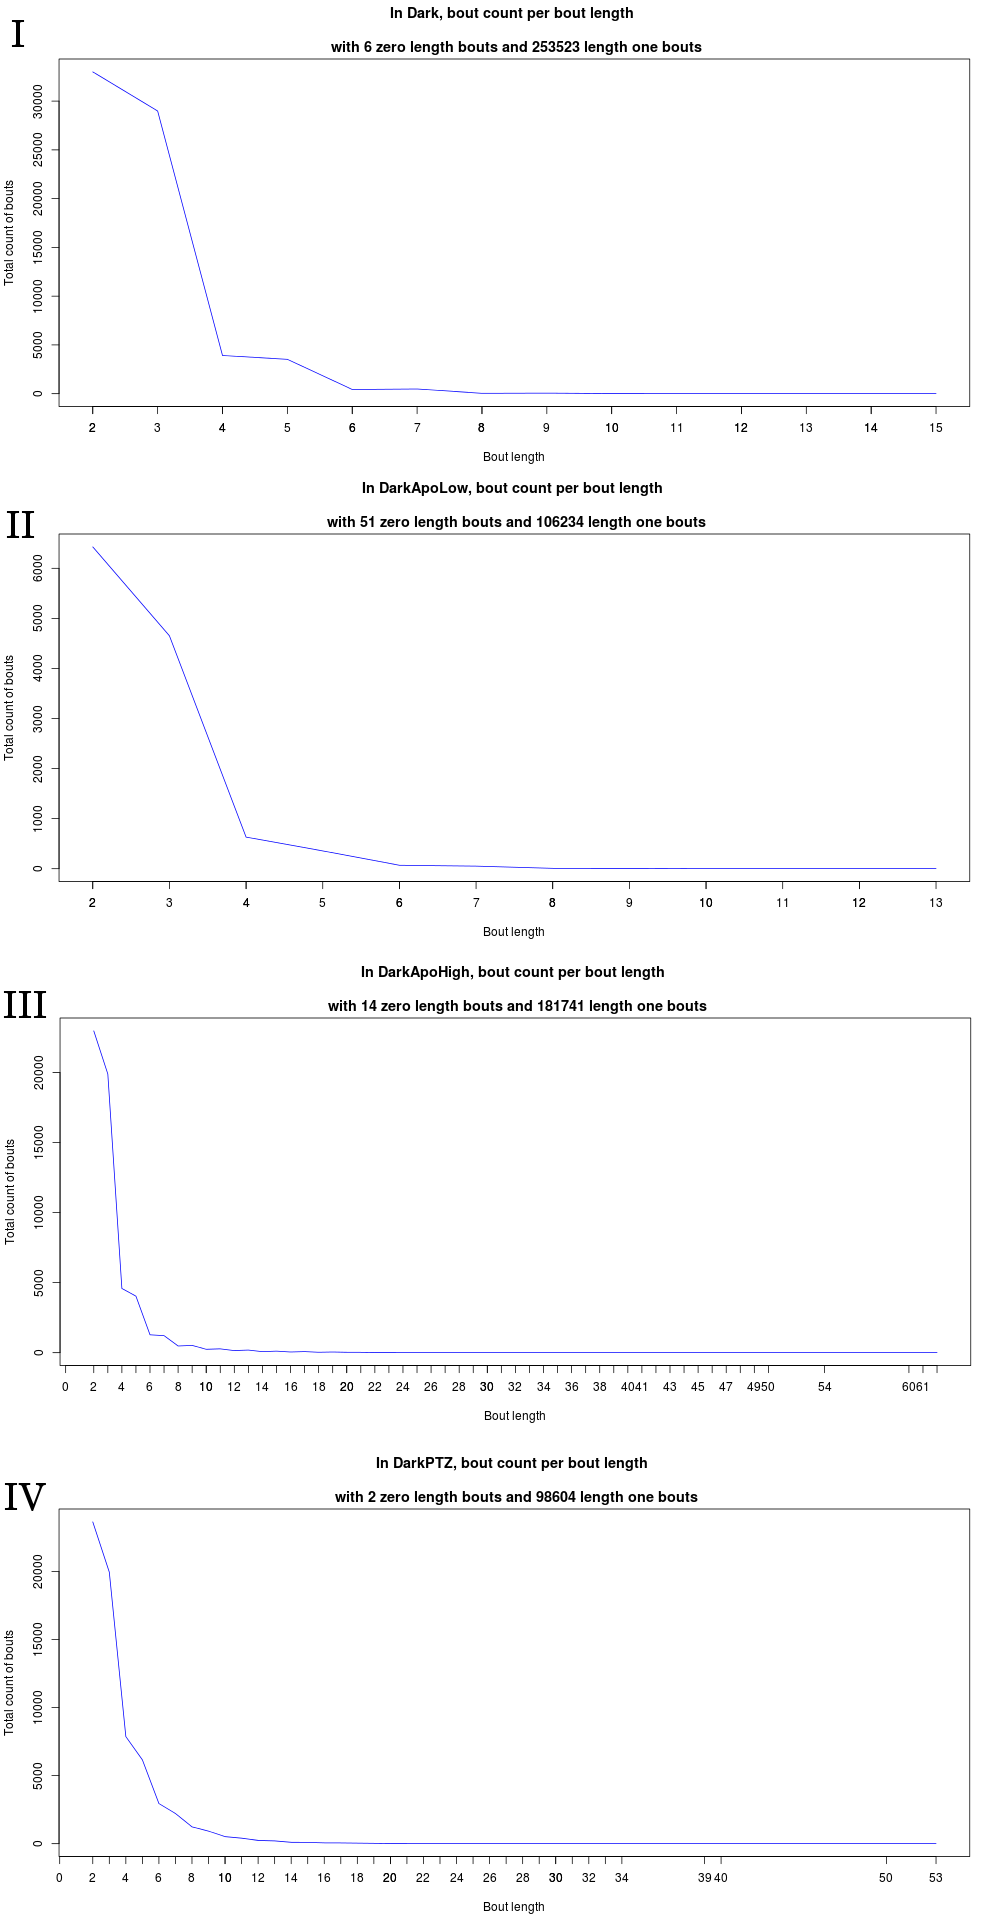
\includegraphics[width=9cm,height=16cm]{TotalBoutCount.png}
\caption{Total bout count per bout length in the control of the healthy(I), the hypoactive(II), the type I hyperactive(III) and the type II hyperactive(IV).}
\end{center}
\end{figure}

\subsubsection{Total bout count per length through time, in each condition}

\begin{figure}[h!]
\begin{center}
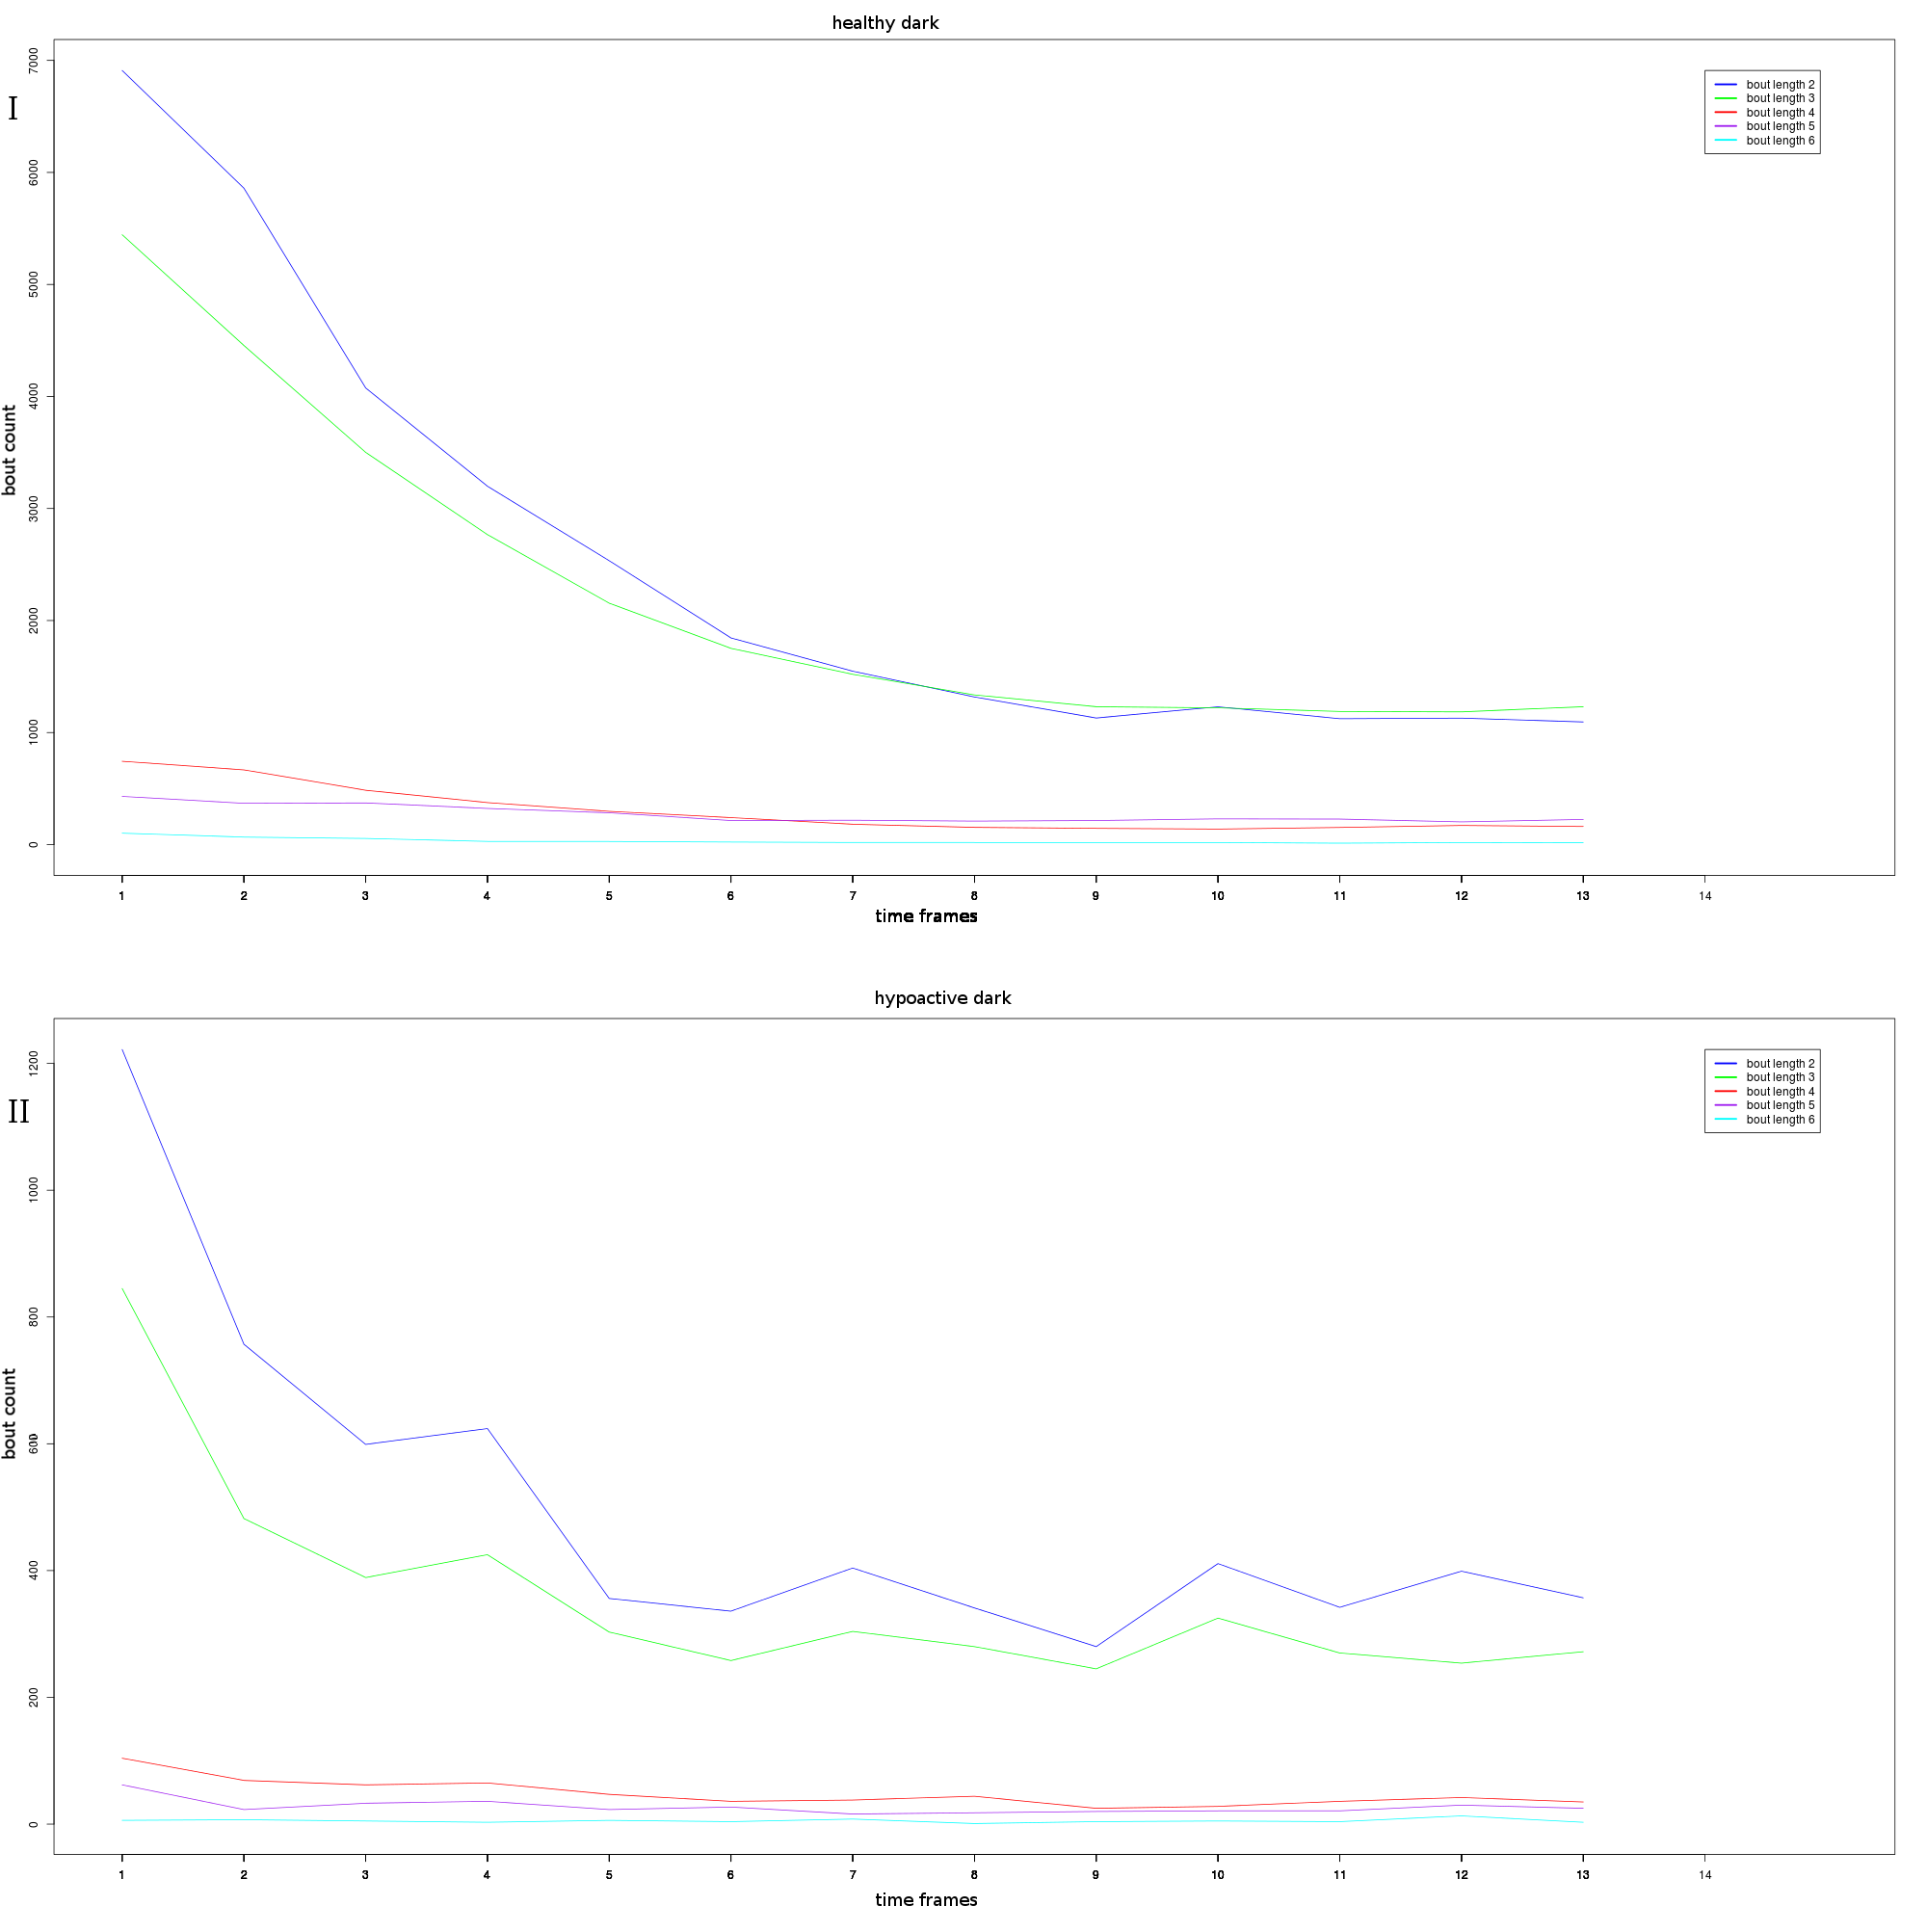
\includegraphics[width=15cm,height=16cm]{countChangeTime1.png}
\end{center}
\end{figure}
\newpage
\begin{figure}[h!]
\begin{center}
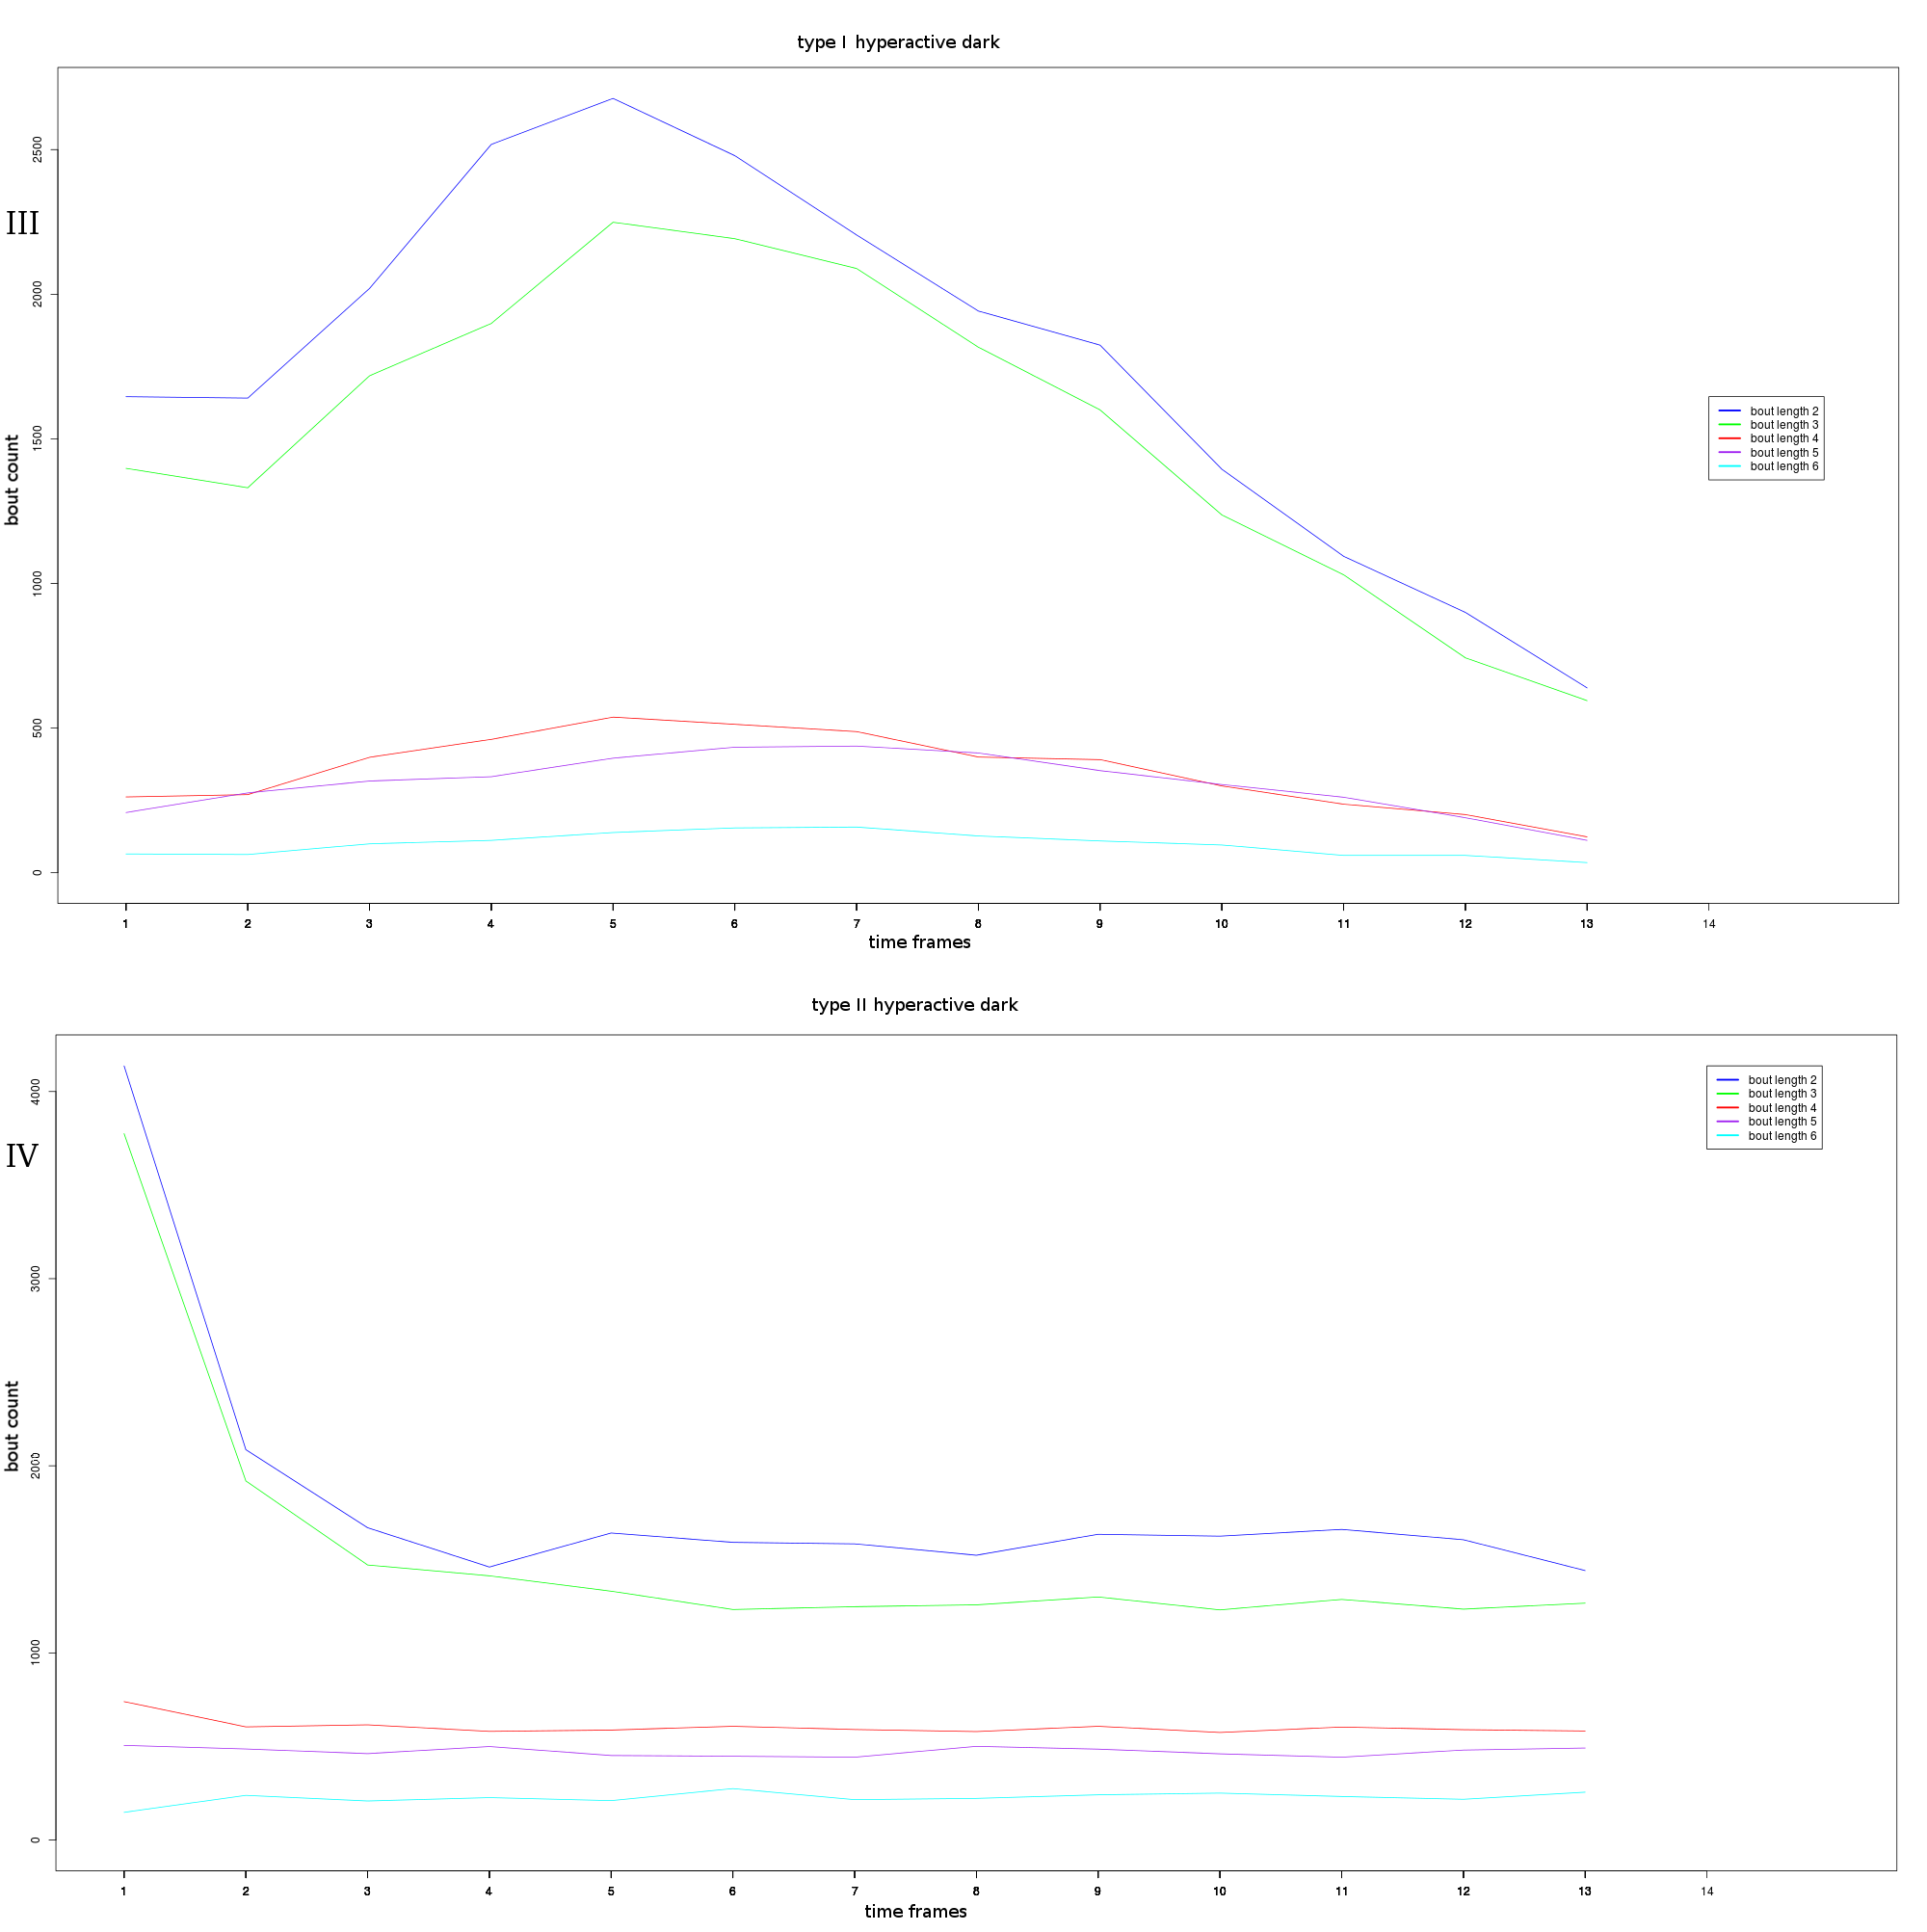
\includegraphics[width=15cm,height=16cm]{countChangeTime2.png}
\caption{Total bout count per bout length through the time frames. Decrease in the control of the healthy(I) can be explained by the larvae falling a sleep, substantial decrease in the control of the hypoactive(II) can be explained by the sedating effect of a low dose of Apomorphine, a u-shape increase, followed by a decrease in total bout count in the control of the type I hyperactive(III) is expected for a high dose of Apomorphine\cite{ref17} and lastly a decrease in the count of short bouts and an increase in the count of longer bouts in the control of the type II hyperactive(IV) is expected when inducing seizures\cite{ref14}.}
\end{center}
\end{figure}


\subsection{Turn proportions}

\subsubsection{Turn proportions per bout length in each condition}

\begin{figure}[h!]
\begin{center}
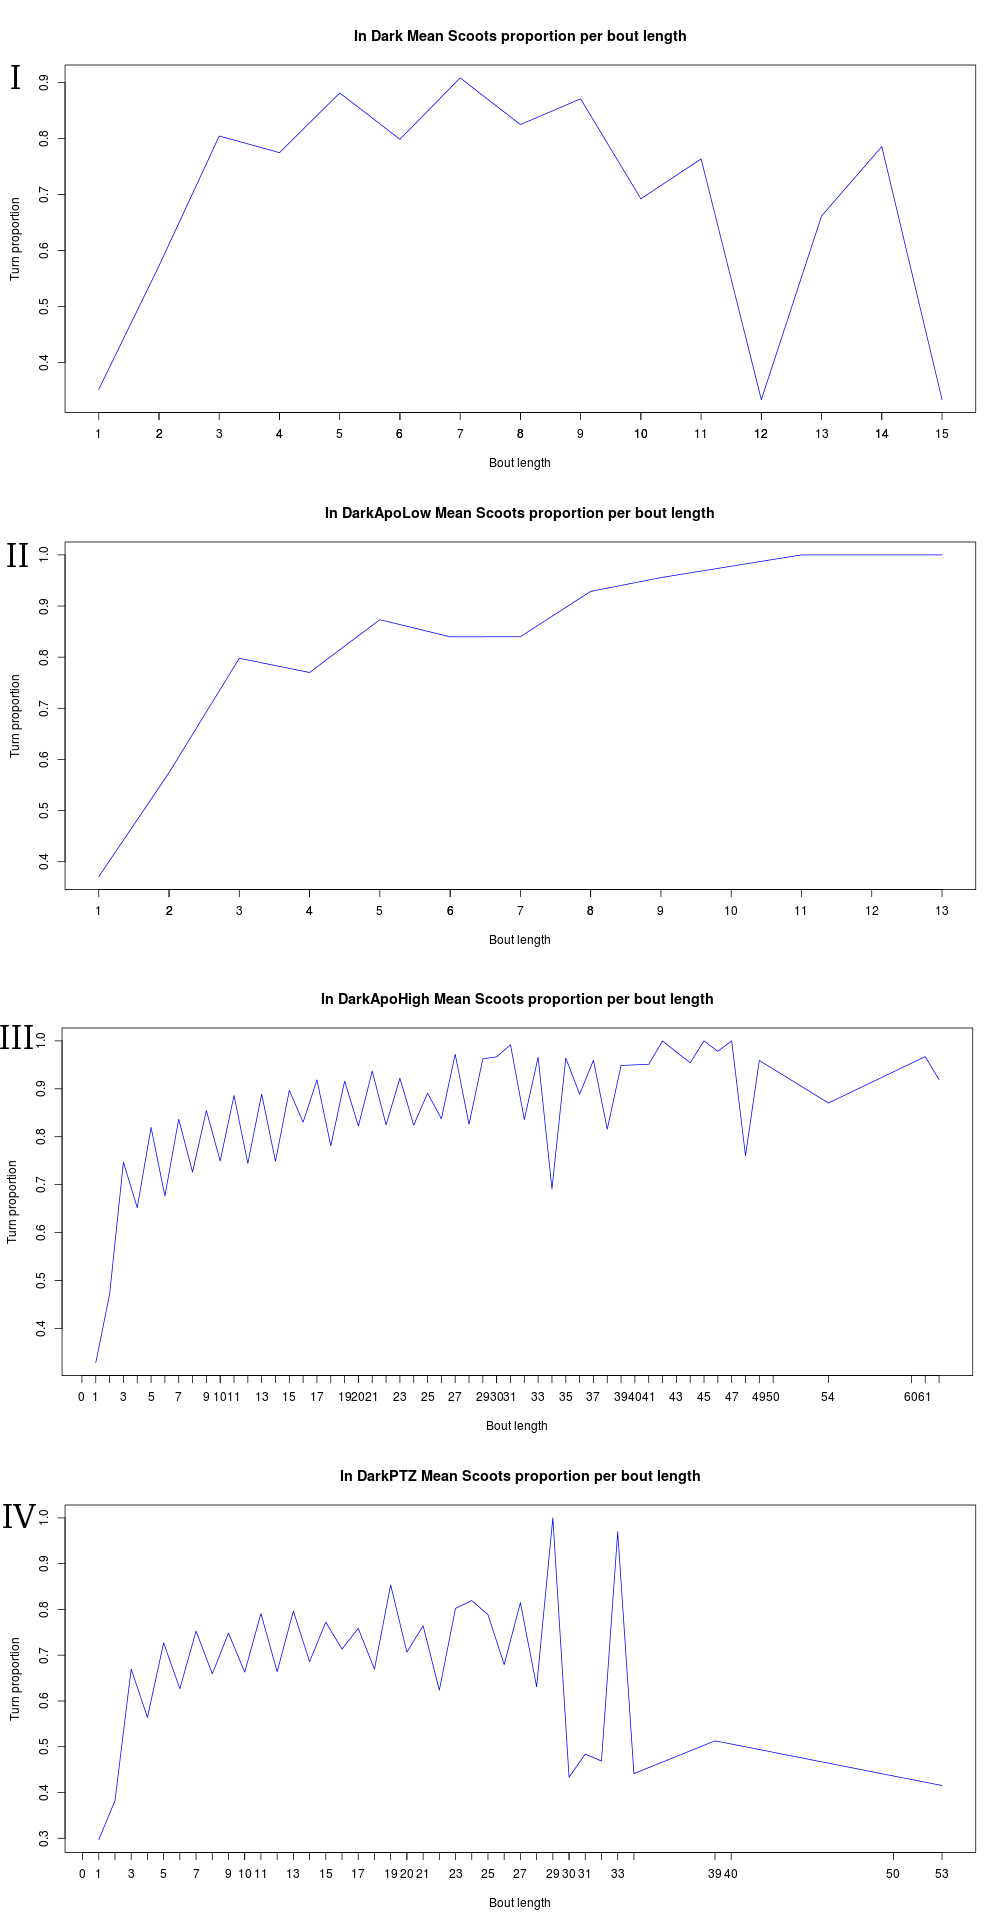
\includegraphics[width=10cm,height=17cm]{boutlengthturnproportion.png}
\caption{Proportions of scoots per bout length in the control of the healthy(I), the hypoactive(II), the type I hyperactive(III) and the type II hyperactive(IV).}
\end{center}
\end{figure}
\newpage
\subsubsection{Turn proportions in bout length strata, through the time frames, in each condition}
\begin{figure}[h!]
\begin{center}
\caption{Comparing compound effects in the hypoactive disease induced condition and the healthy condition. 10 $\mu$M Haloperidol effects in length 2 bout counts(I) and length 2 scoots proportions(II), the effects of 10 $\mu$M Clozapine in length 2 bout counts(III) and length 2 scoots proportions(IV) and the effects of 100 $\mu$M NDMC in length 2 bout counts(V) and length 2 scoots proportions(VI).}
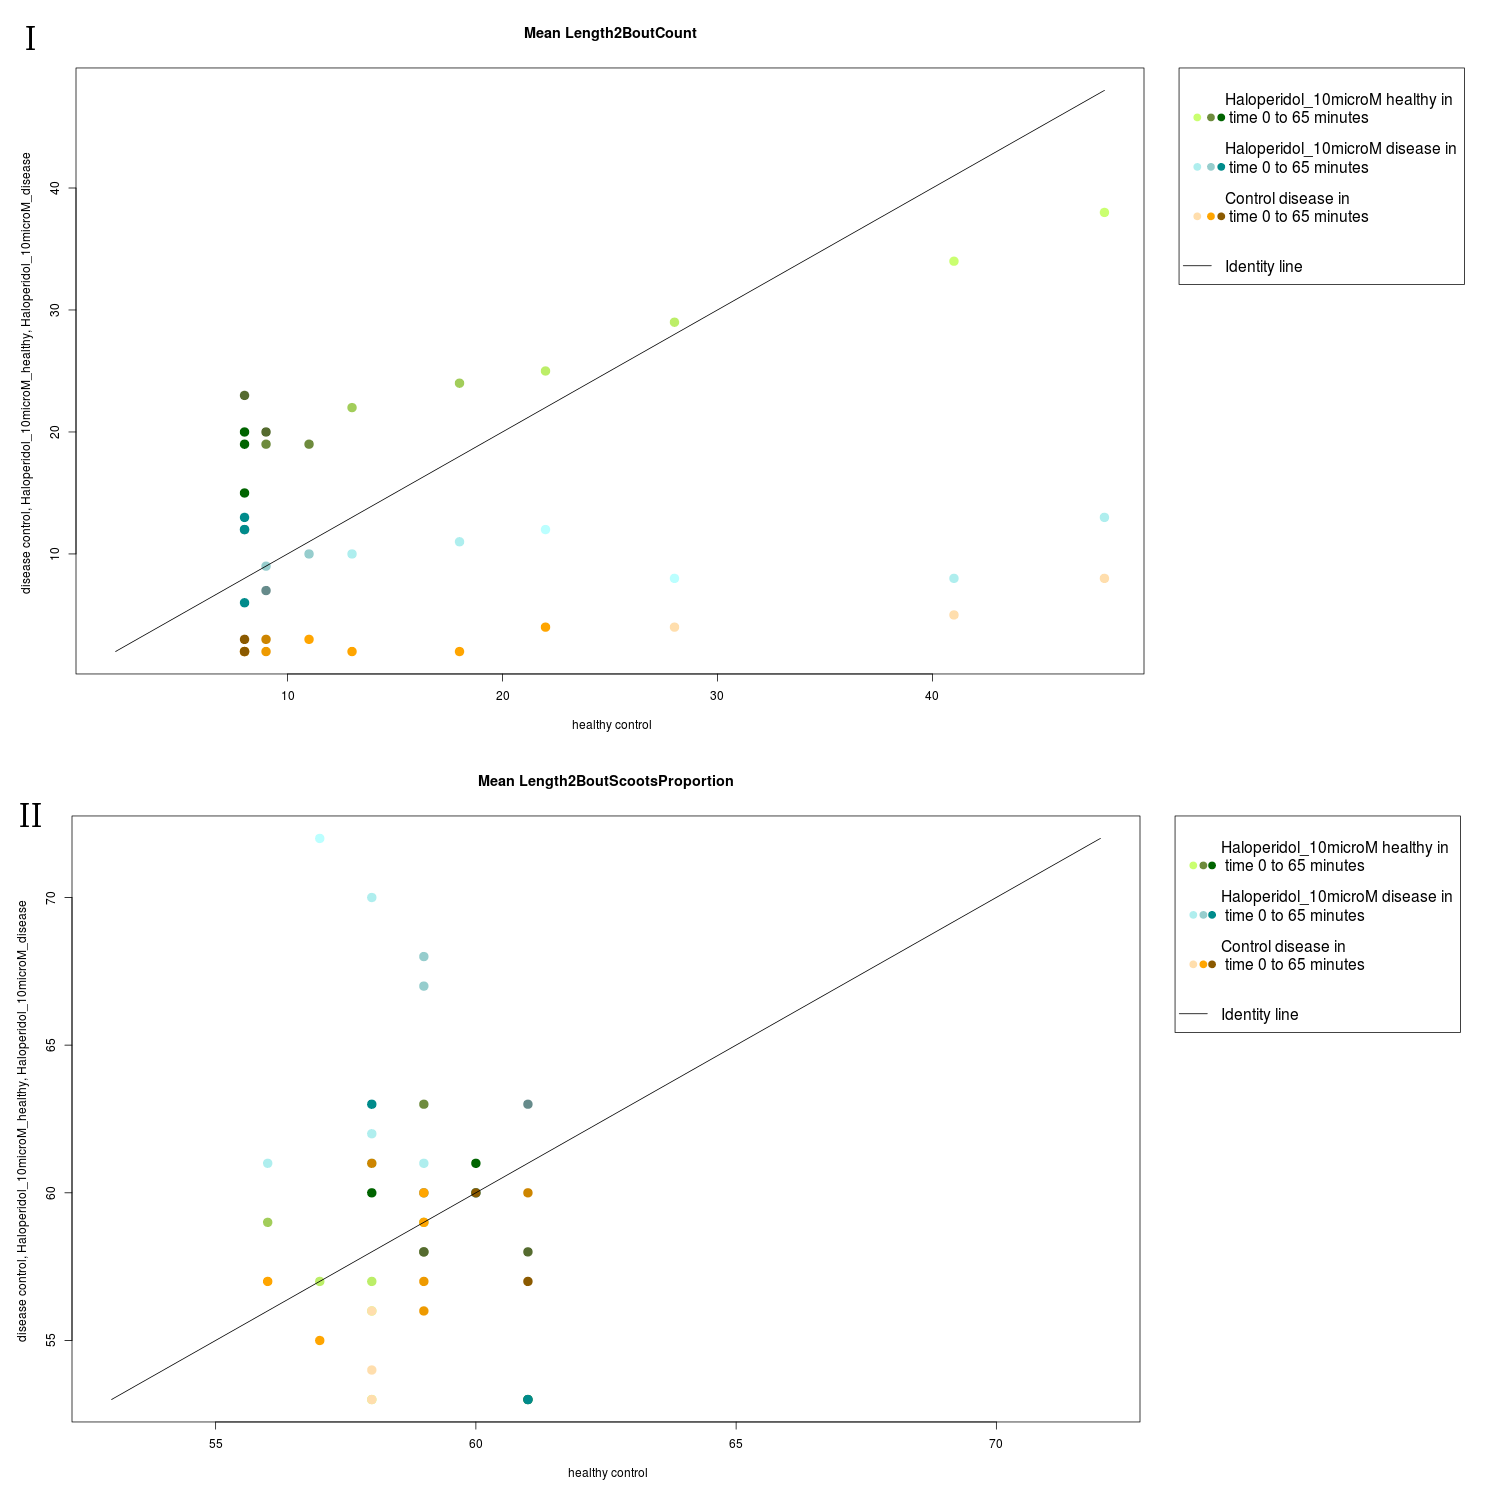
\includegraphics[width=15cm,height=16cm]{ApoLowCountScootsH.png}
\end{center}
\end{figure}
\newpage
\begin{figure}[h!]
\begin{center}
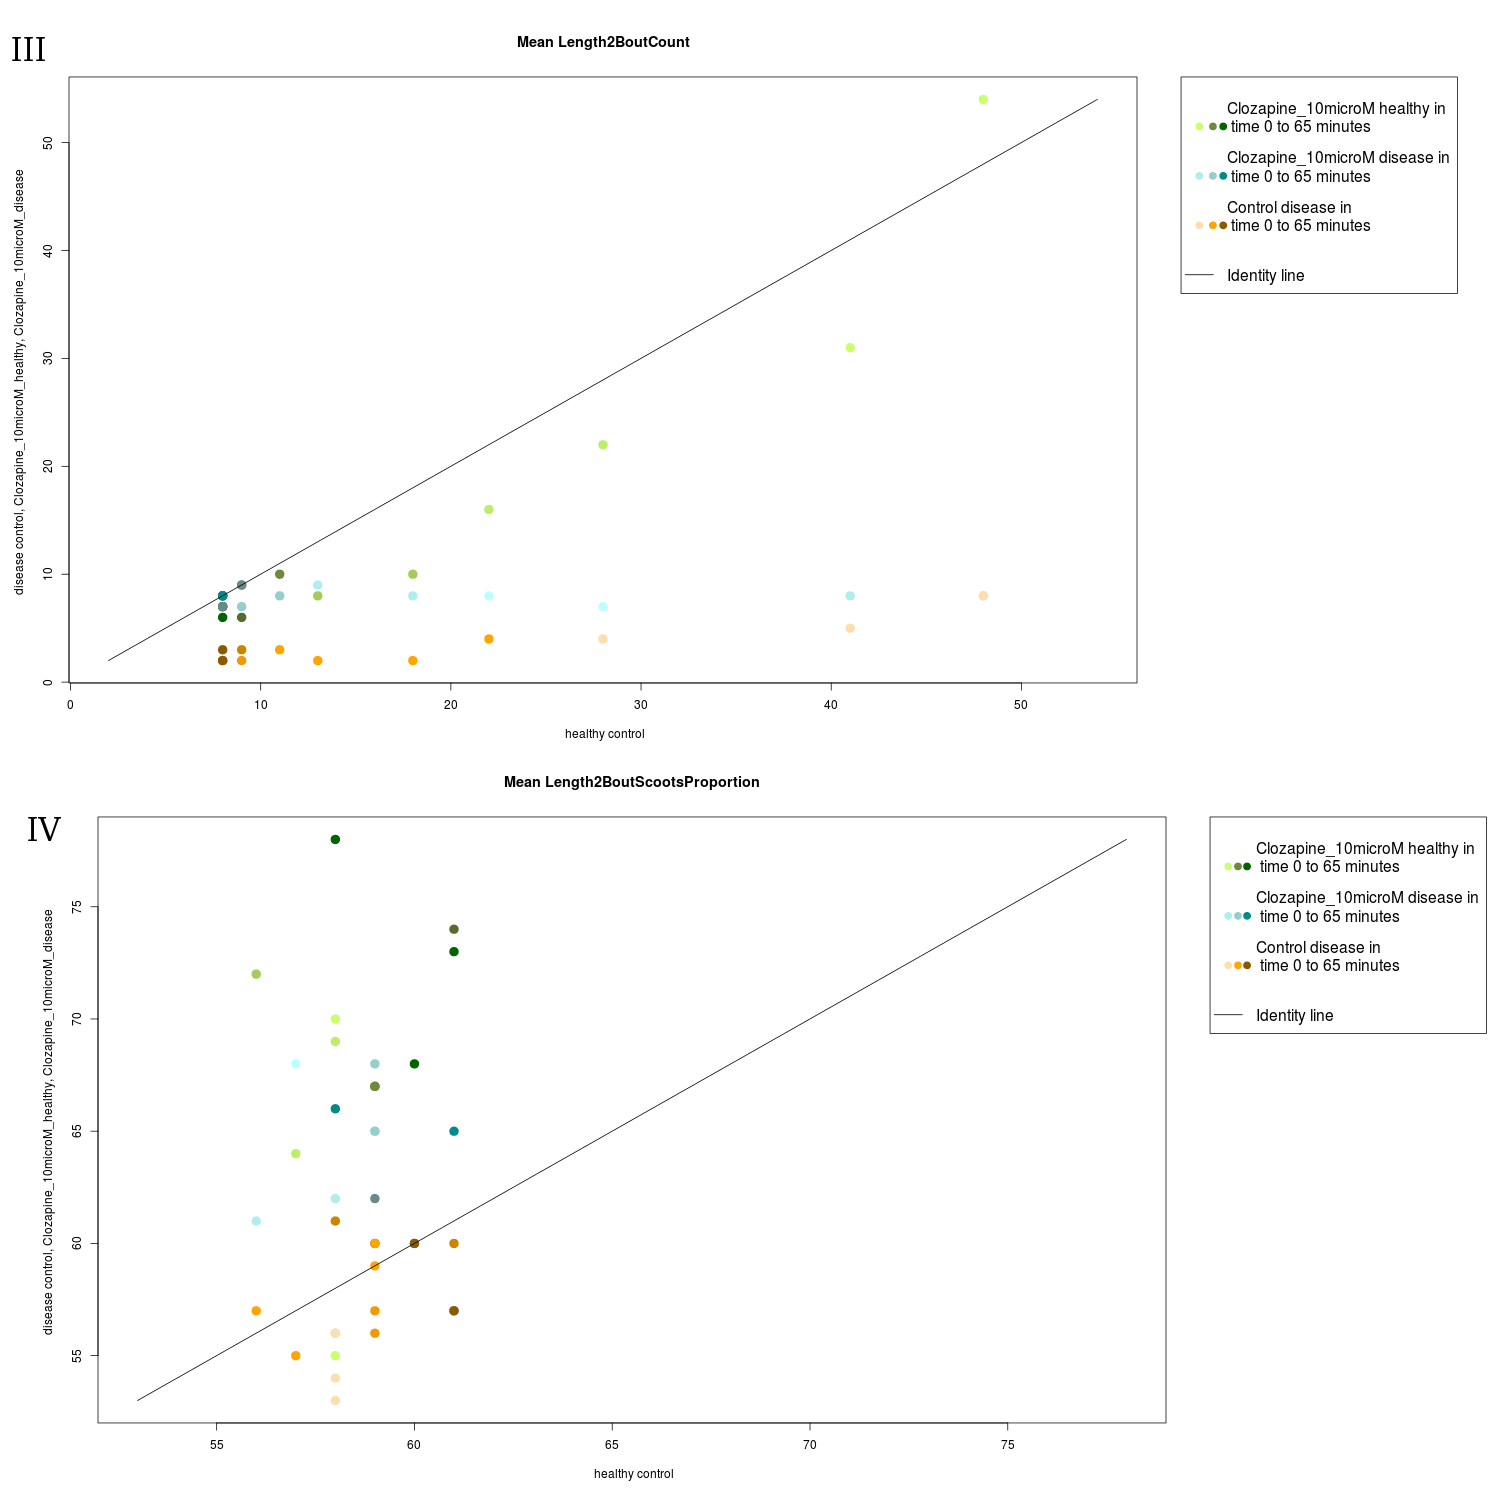
\includegraphics[width=15cm,height=16cm]{ApoLowCountScootsC.png}
\end{center}
\end{figure}
\newpage
\begin{figure}[h!]
\begin{center}
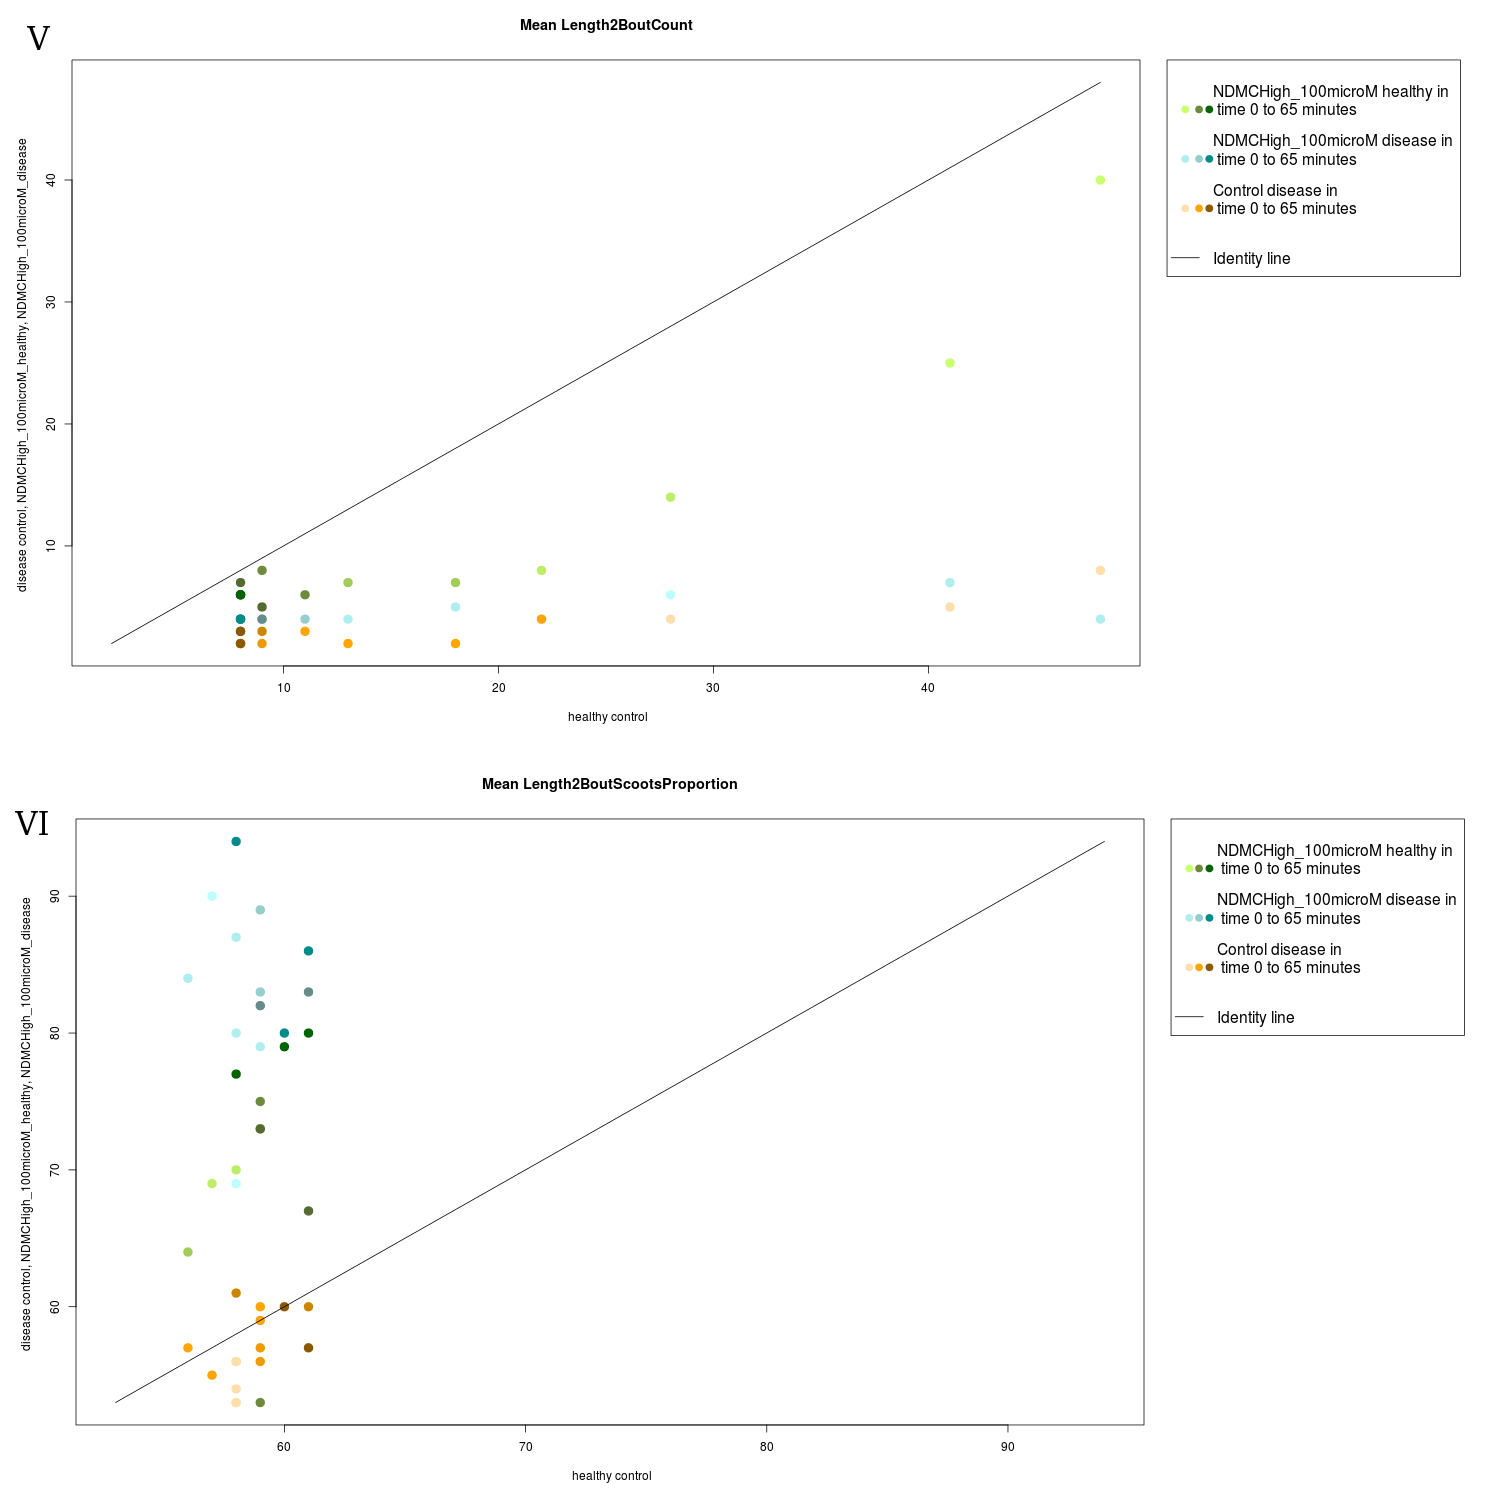
\includegraphics[width=15cm,height=16cm]{ApoLowCountScootsN.png}
\end{center}
\end{figure}



\newpage
\begin{figure}[h!]
\begin{center}
\caption{Comparing compound effects in the type I hyperactive disease induced condition and the healthy condition. 10 $\mu$M Haloperidol effects in length 2 bout counts(I) and length 2 scoots proportions(II), the effects of 10 $\mu$M Clozapine in length 2 bout counts(III) and length 2 scoots proportions(IV) and the effects of 100 $\mu$M NDMC in length 2 bout counts(V) and length 2 scoots proportions(VI).}
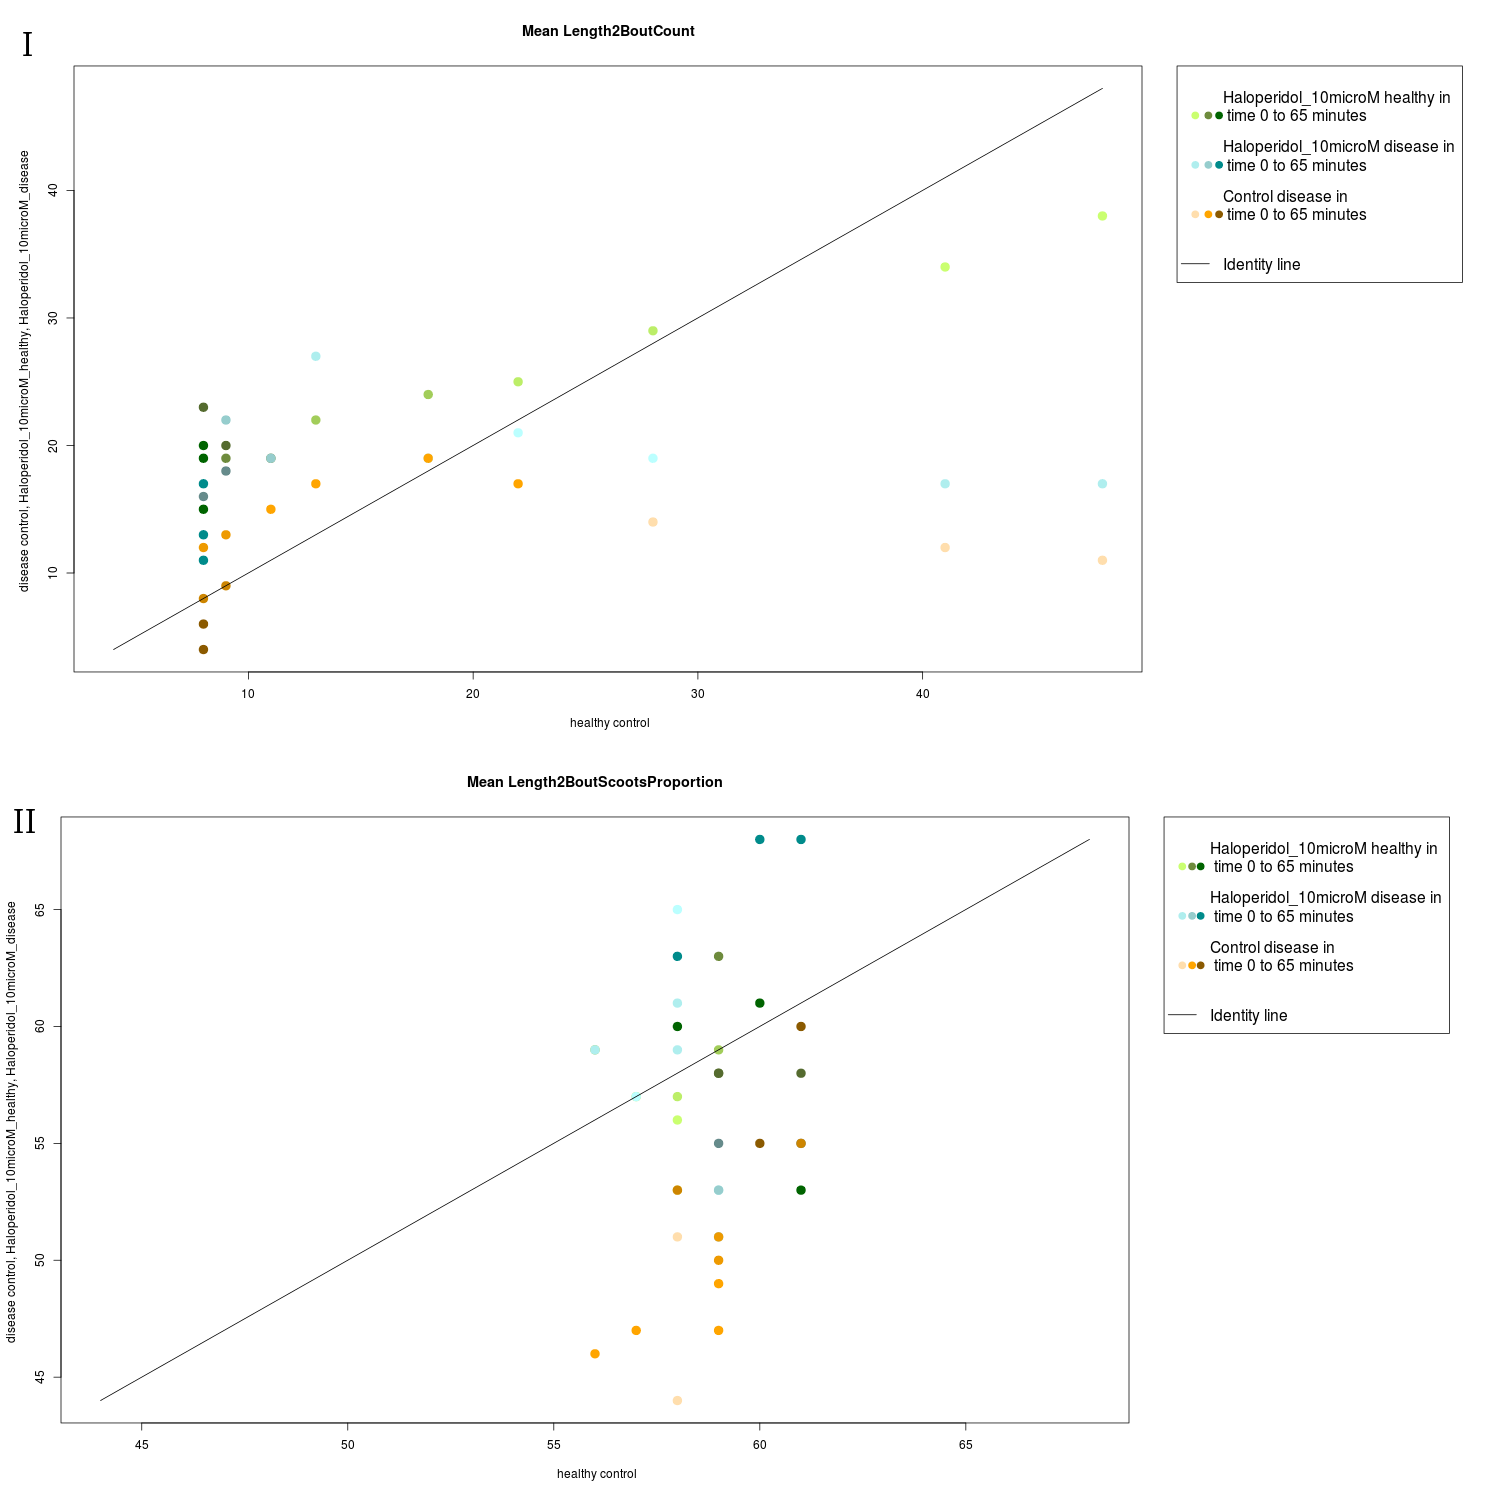
\includegraphics[width=15cm,height=16cm]{ApoHighCountScootsH.png}
\end{center}
\end{figure}
\newpage
\begin{figure}[h!]
\begin{center}
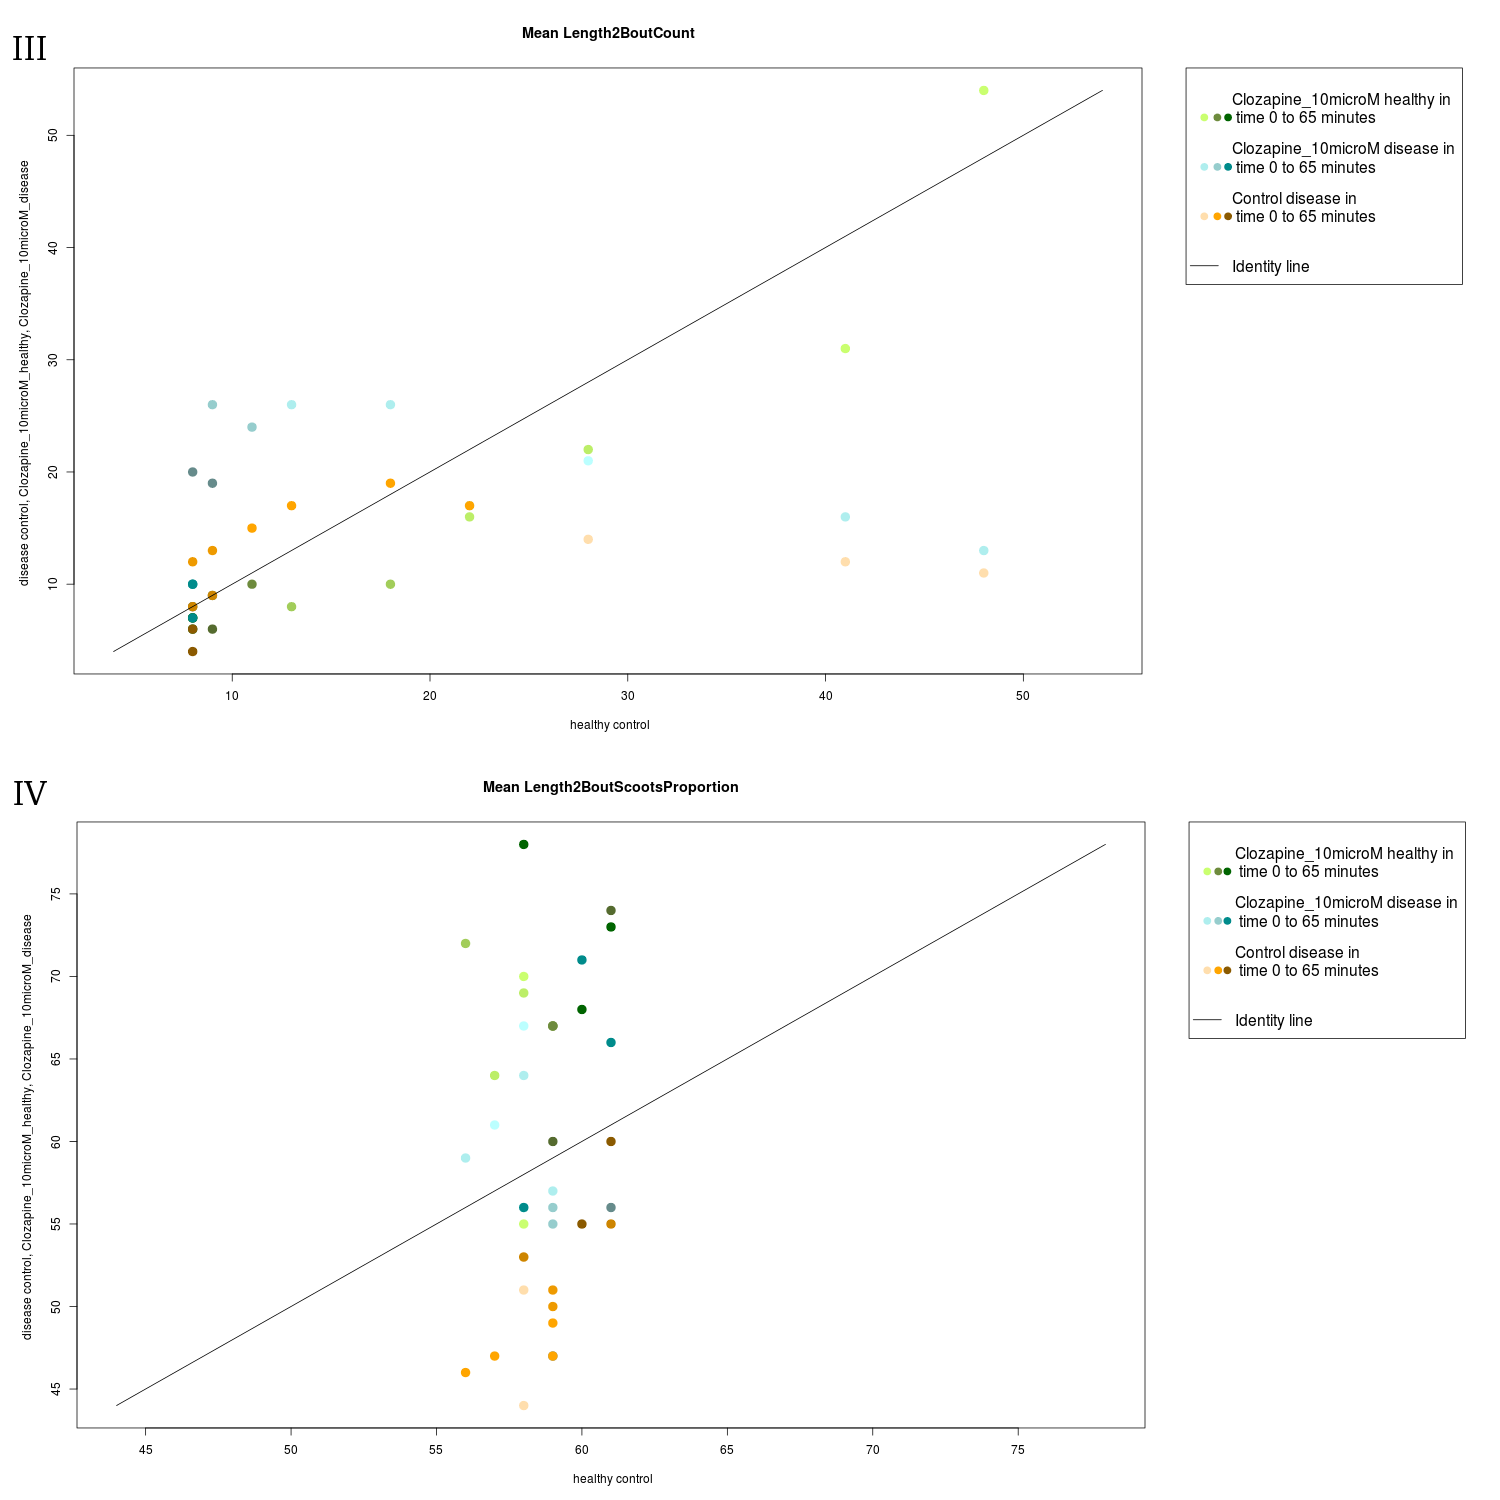
\includegraphics[width=15cm,height=16cm]{ApoHighCountScootsC.png}
\end{center}
\end{figure}
\newpage
\begin{figure}[h!]
\begin{center}
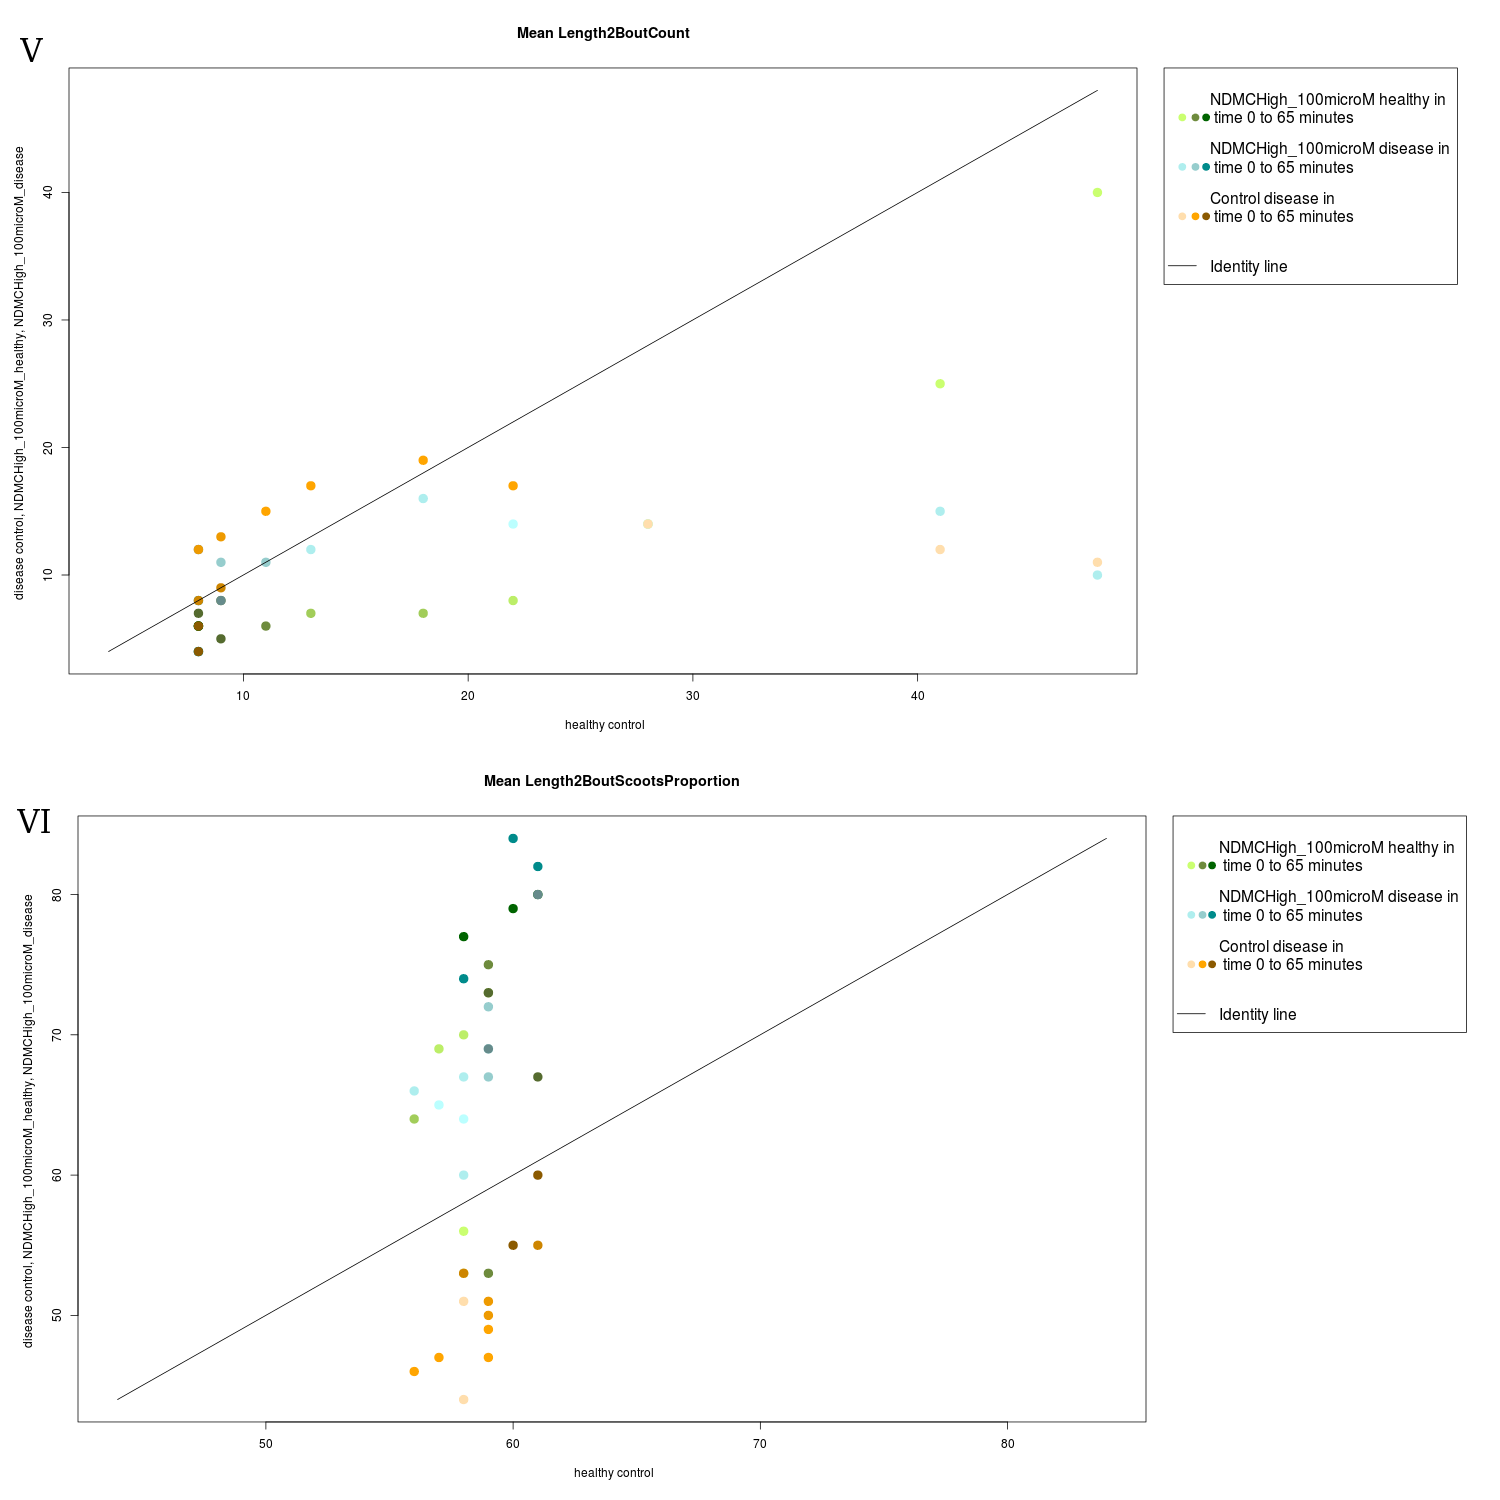
\includegraphics[width=15cm,height=16cm]{ApoHighCountScootsN.png}
\end{center}
\end{figure}



\newpage
\begin{figure}[h!]
\begin{center}
\caption{Comparing compound effects in the type II hyperactive disease induced condition and the healthy condition. 10 $\mu$M Haloperidol effects in length 2 bout counts(I) and length 2 scoots proportions(II), the effects of 10 $\mu$M Clozapine in length 2 bout counts(III) and length 2 scoots proportions(IV) and the effects of 100 $\mu$M NDMC in length 2 bout counts(V) and length 2 scoots proportions(VI).}
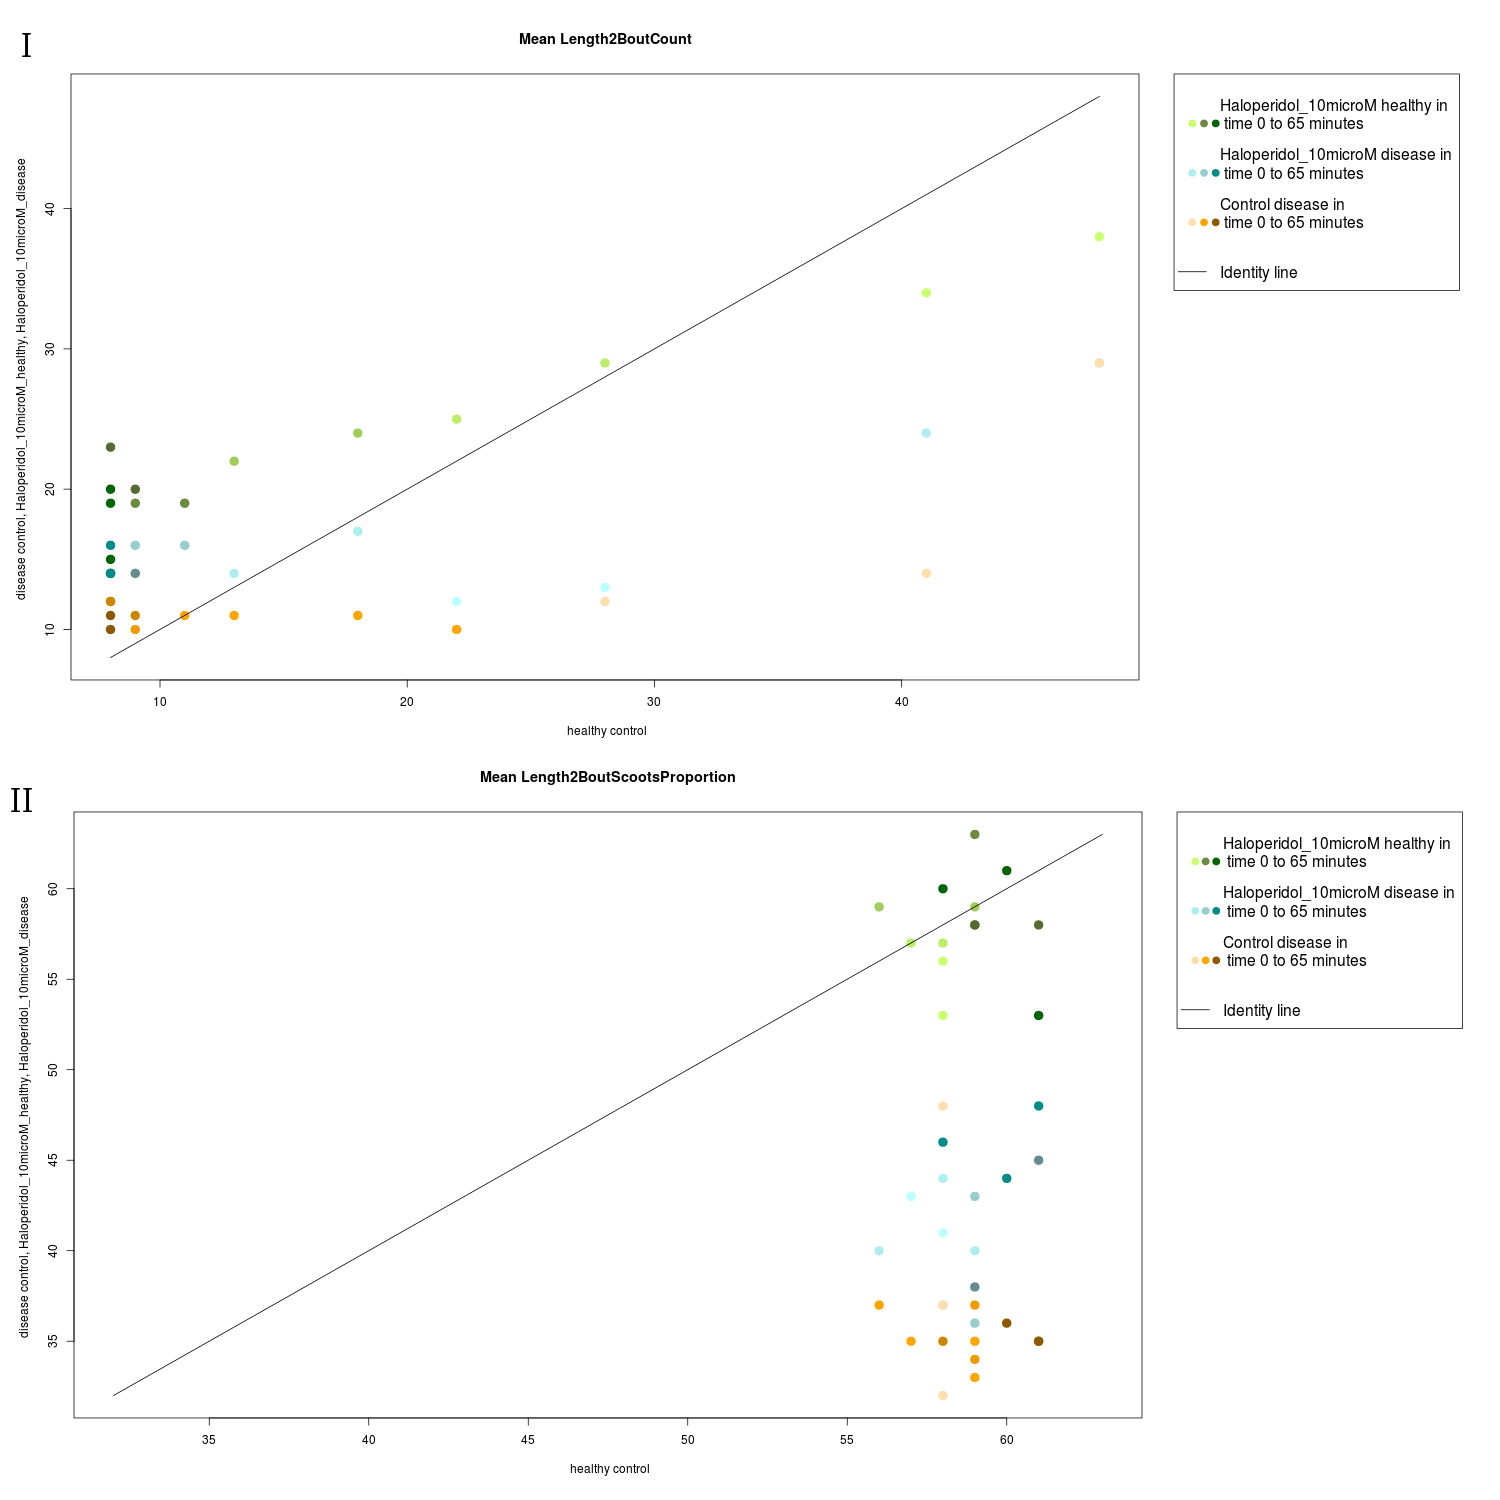
\includegraphics[width=15cm,height=17cm]{PTZCountScootsH.png}
\end{center}
\end{figure}
\newpage
\begin{figure}[h!]
\begin{center}
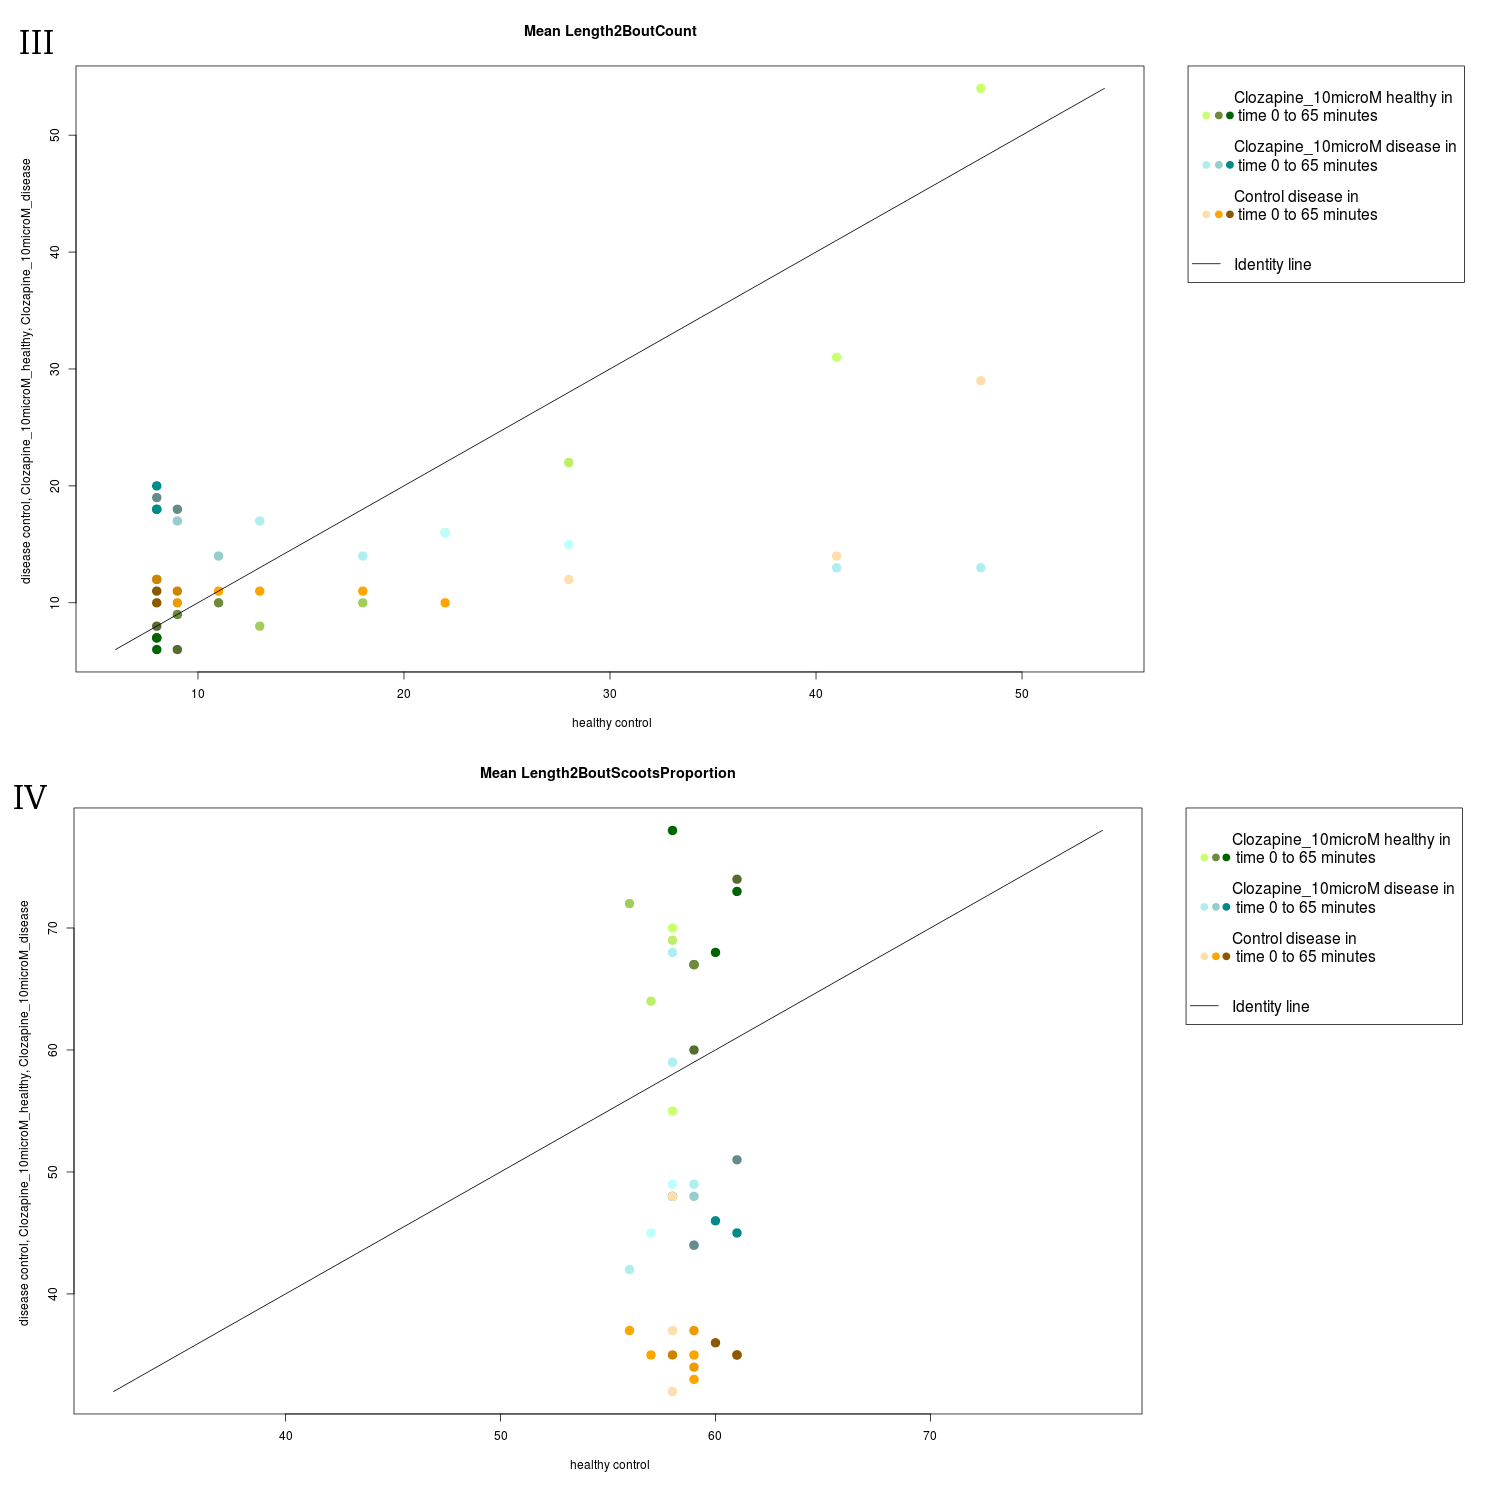
\includegraphics[width=15cm,height=17cm]{PTZCountScootsC.png}
\end{center}
\end{figure}
\newpage
\begin{figure}[h!]
\begin{center}
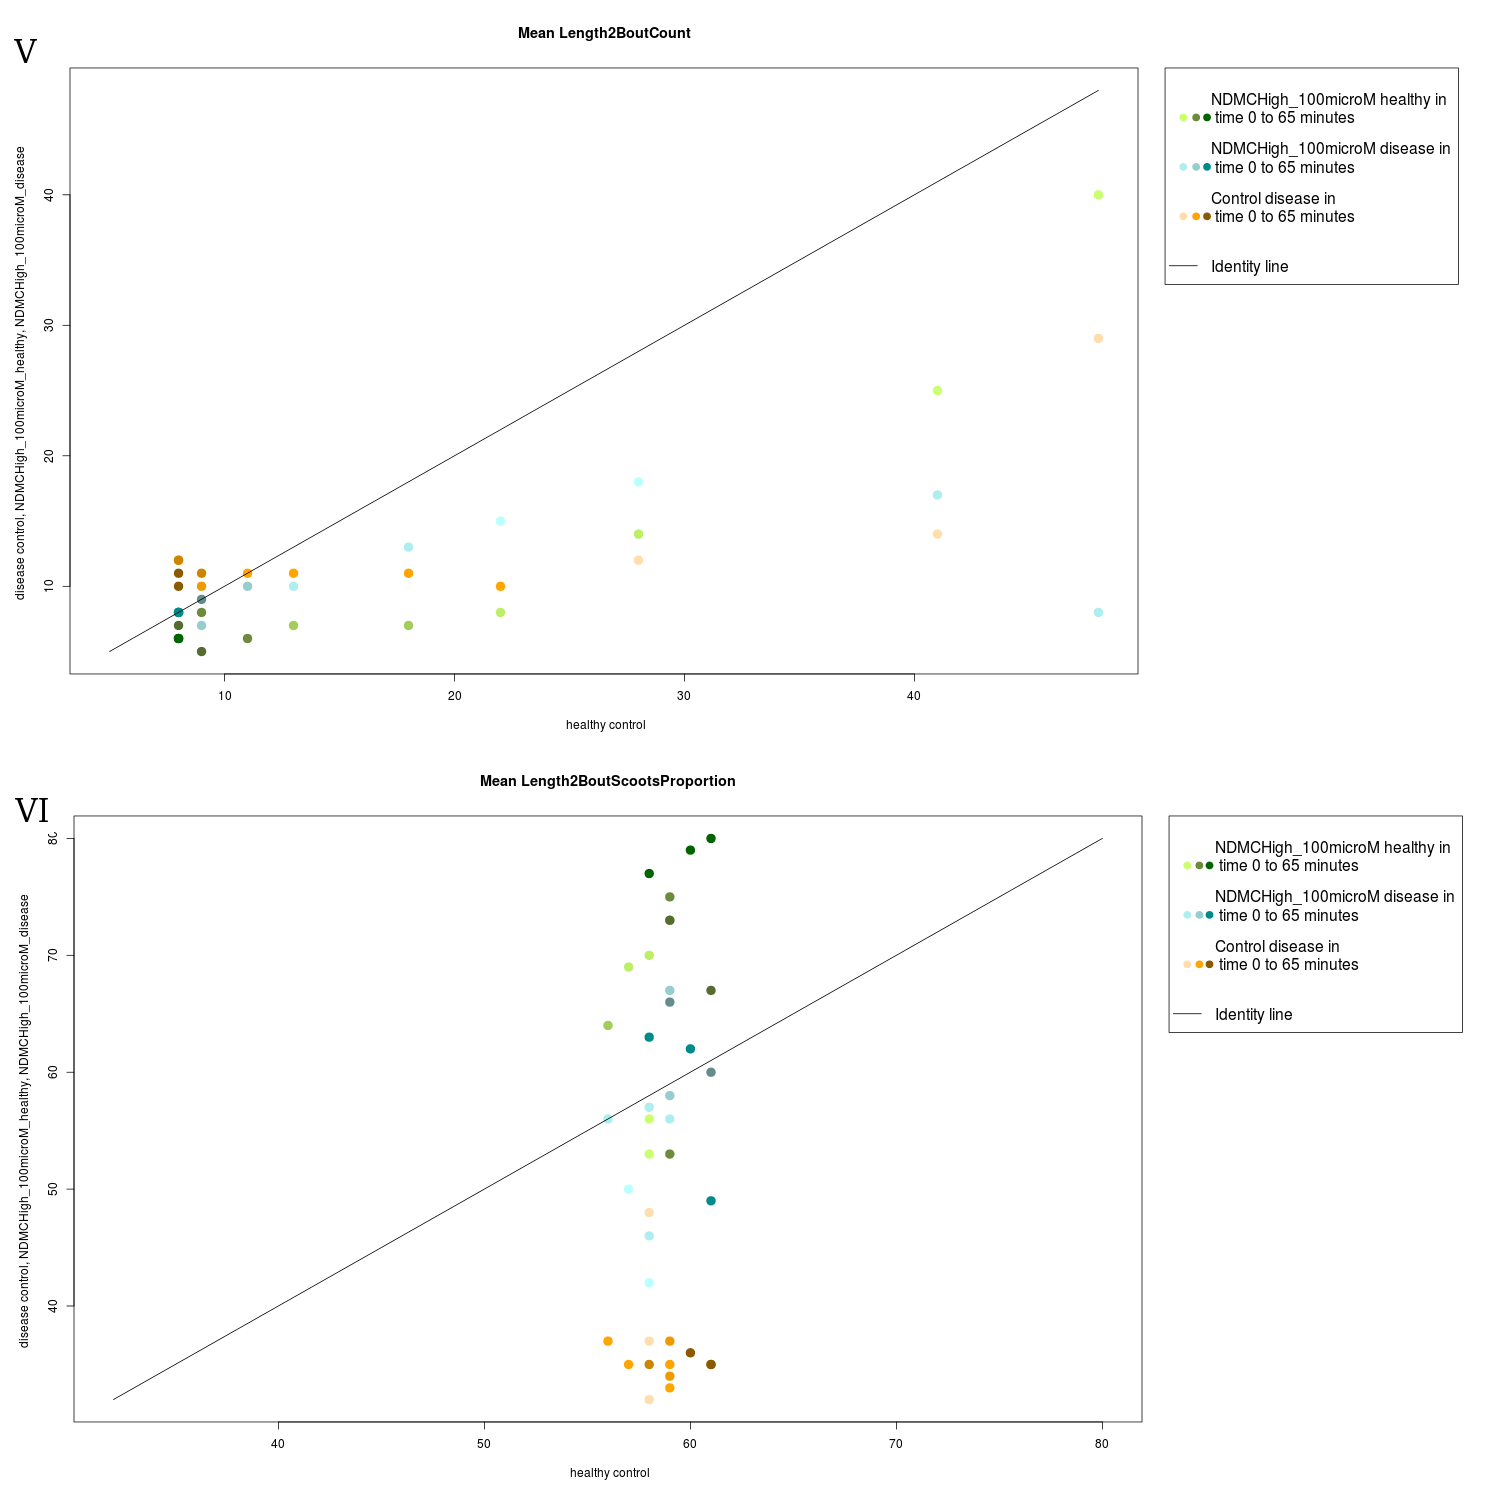
\includegraphics[width=15cm,height=16cm]{PTZCountScootsN.png}
\end{center}
\end{figure}


\newpage
\subsection{Transition proportions}
\subsubsection{Transitions of length 3, in each condition}

\begin{figure}[h!]
\begin{center}
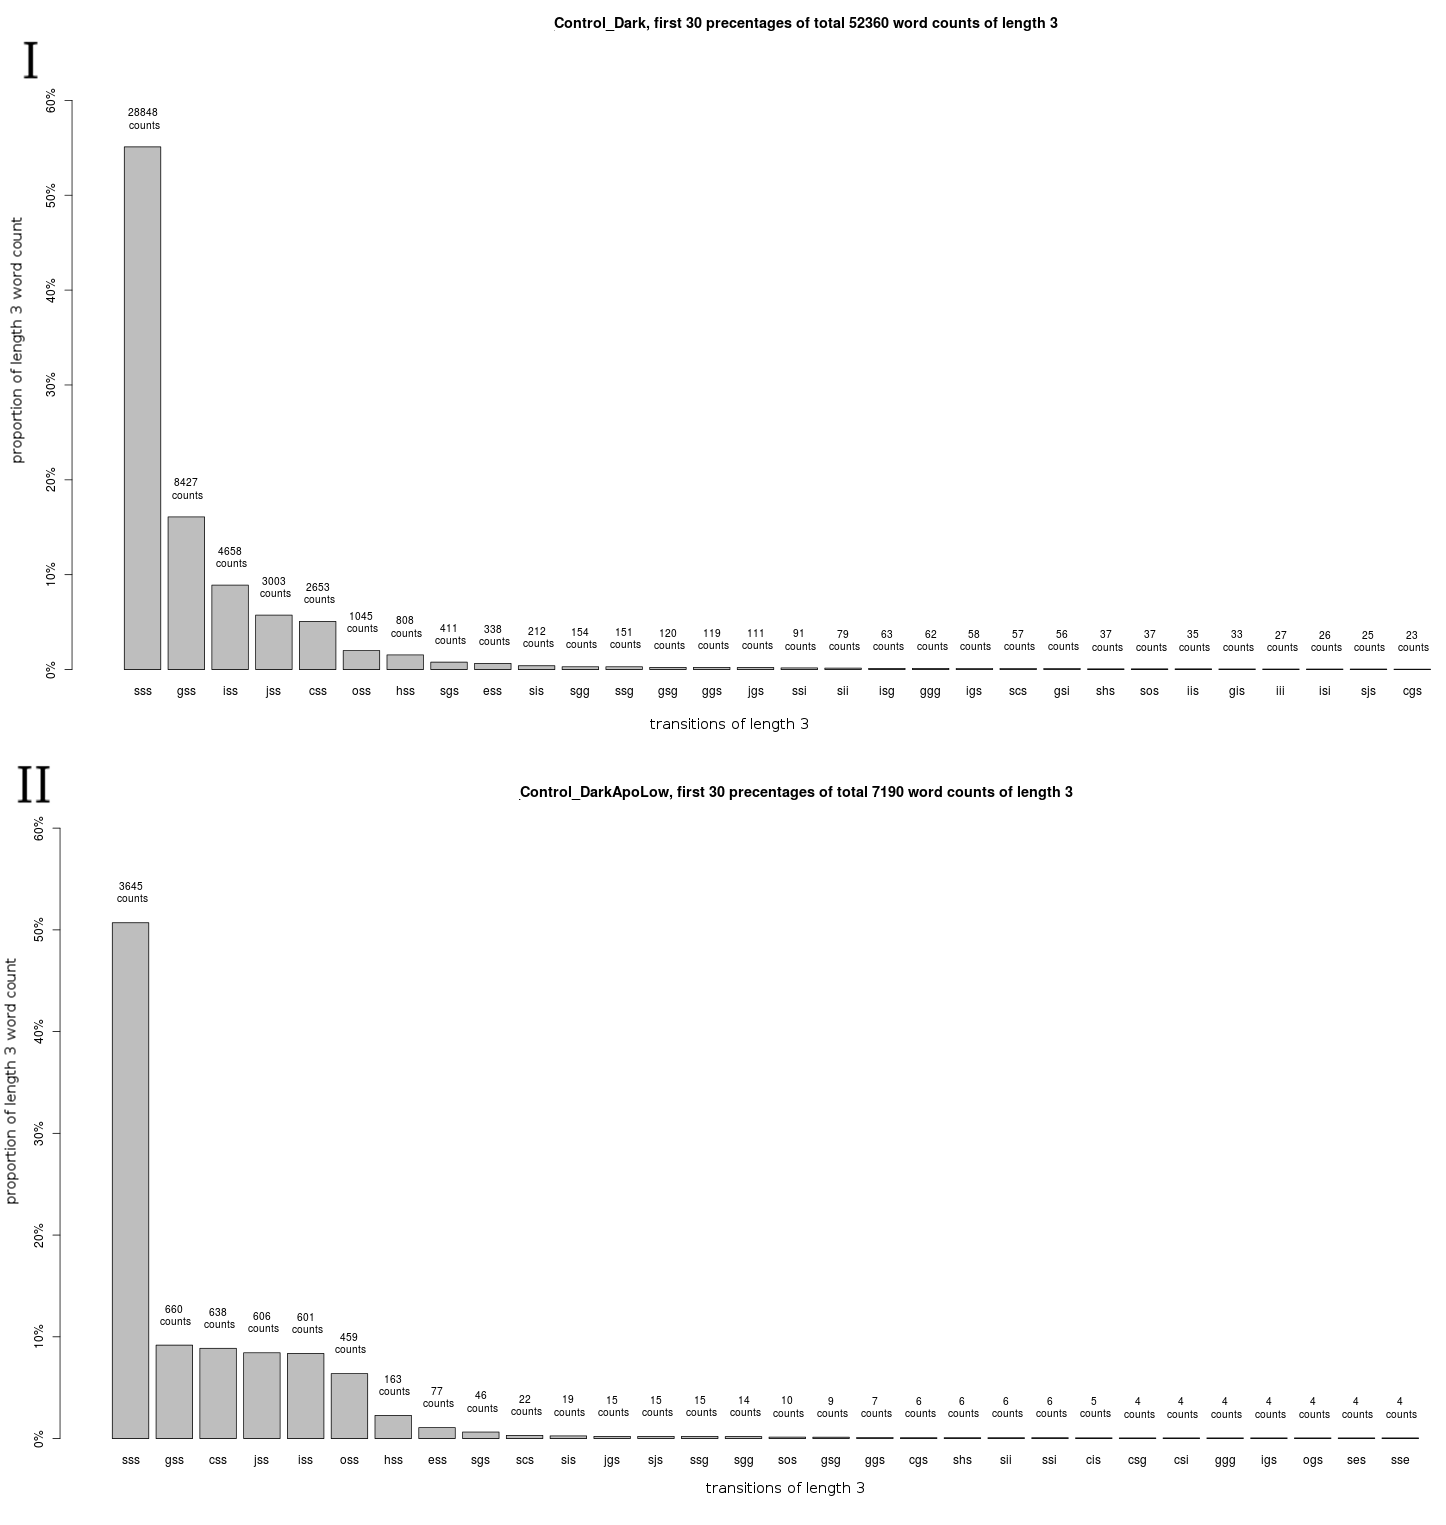
\includegraphics[width=15cm,height=17cm]{transitionsperboutlength1.png}
\end{center}
\end{figure}
\begin{figure}[h!]
\begin{center}
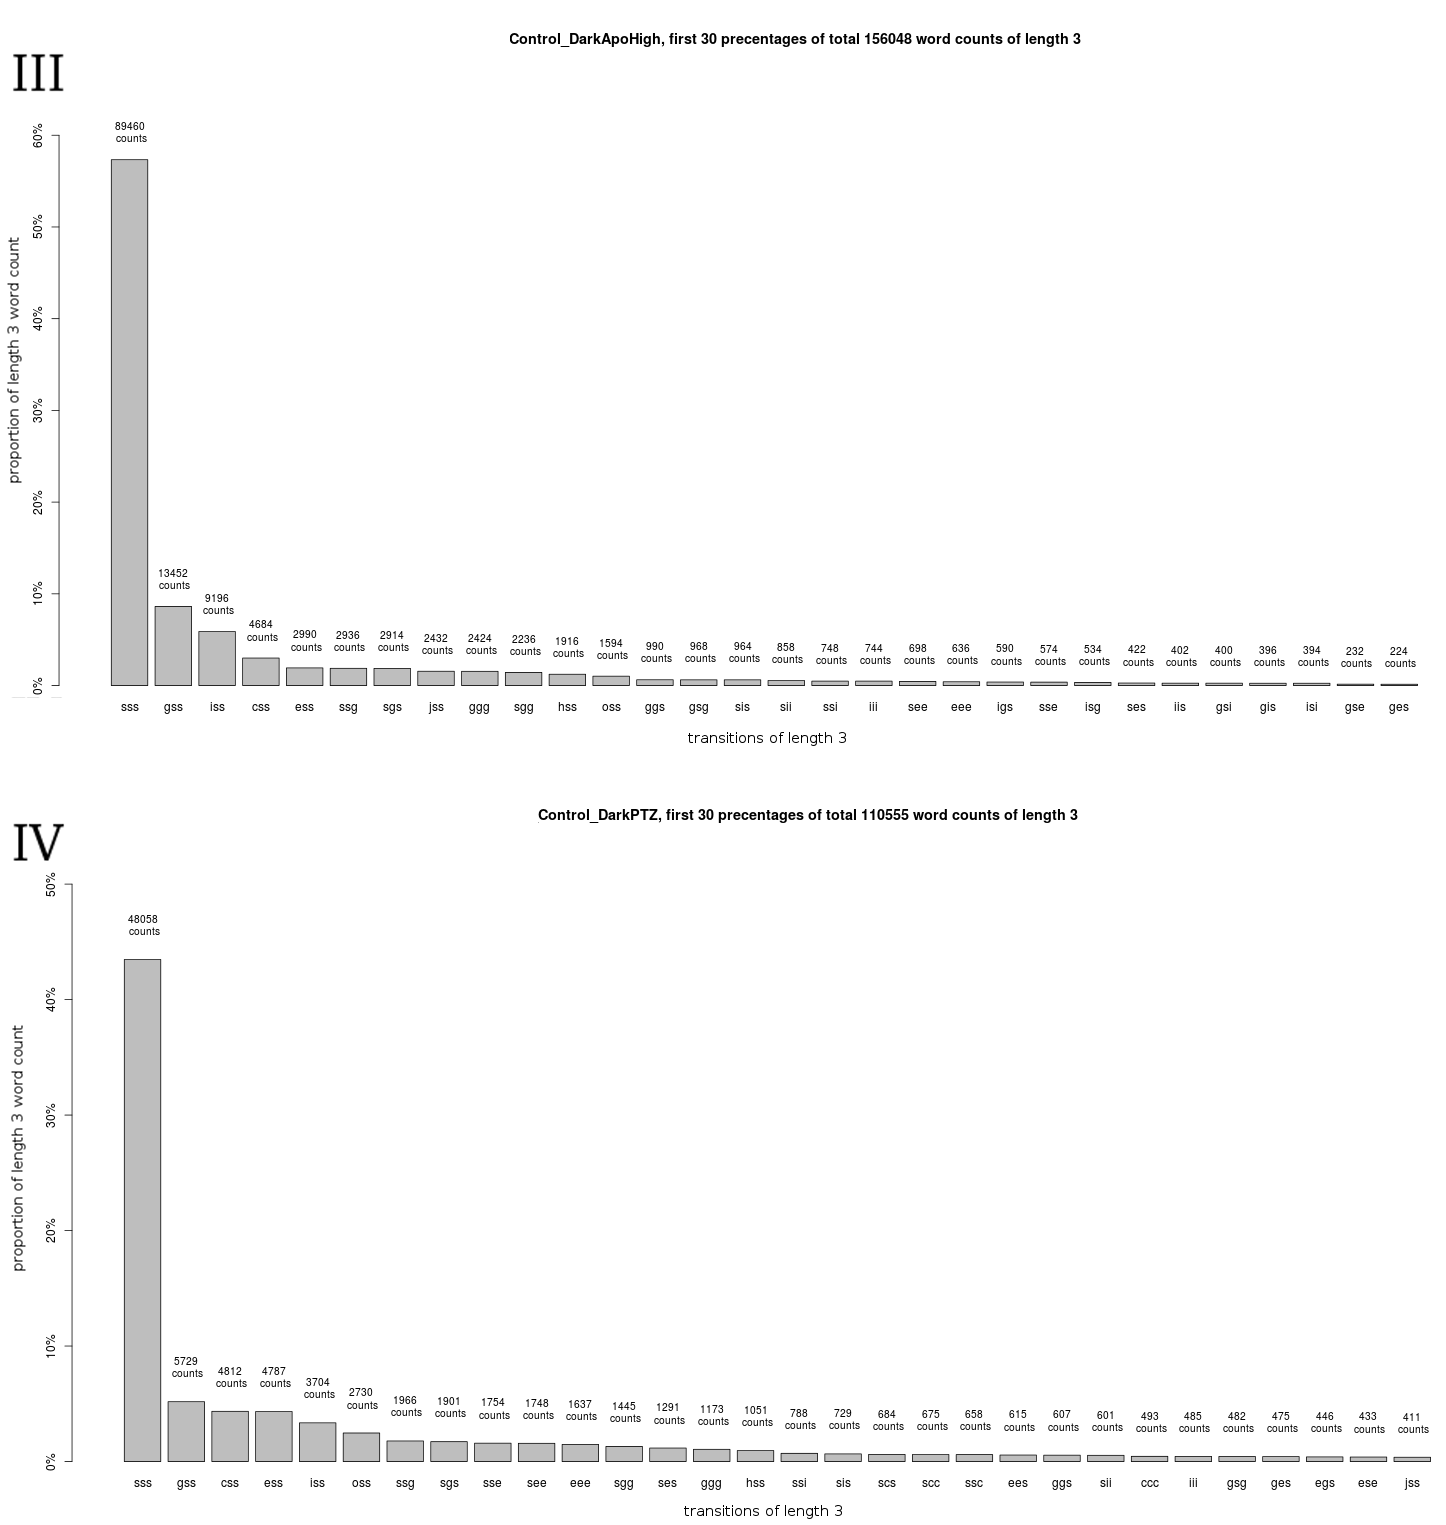
\includegraphics[width=15cm,height=17cm]{transitionsperboutlength2.png}
\caption{Proportions of transitions of length 3 in the control of the healthy(I), the hypoactive(II), the type I hyperactive(III) and the type II hyperactive(IV).}
\end{center}
\end{figure}

\section{Exploratory data analysis appendix}

\subsection{PCA plots}

\includepdf[pages=-]{DarkApoLow_1.pdf}
\includepdf[pages=-]{DarkApoHigh_1.pdf}
\includepdf[pages=-]{DarkPTZ_1.pdf}

\includepdf[pages=-]{DarkApoLow_2.pdf}
\includepdf[pages=-]{DarkApoHigh_2.pdf}
\includepdf[pages=-]{DarkPTZ_2.pdf}


\includepdf[pages=-]{DarkApoLow_3.pdf}
\includepdf[pages=-]{DarkApoHigh_3.pdf}
\includepdf[pages=-]{DarkPTZ_3.pdf}


\includepdf[pages=-]{DarkApoLow_4.pdf}
\includepdf[pages=-]{DarkApoHigh_4.pdf}
\includepdf[pages=-]{DarkPTZ_4.pdf}

\subsection{Most influential variables in PCA}
\begin{table}[h!]\tiny
\centering
\begin{tabular}{|c|c|c|c|}
\hline
                                                    & \begin{tabular}[c]{@{}c@{}}hypoactive\\condition\end{tabular}                &\begin{tabular}[c]{@{}c@{}} type I hyperactive\\condition \end{tabular}              & \begin{tabular}[c]{@{}c@{}}type II hyperactive\\condition\end{tabular}                \\ \hline
\begin{tabular}[c]{@{}c@{}c@{}c@{}c@{}}First 20\\most influential\\descriptive\\statistics\\\end{tabular} & C-Bends Proportion                  & E-Bends Proportion                  & E-Bends Proportion                  \\ \cline{2-4} 
\begin{tabular}[c]{@{}c@{}c@{}c@{}} \\ \\ \\\end{tabular}                                                    & Scoots Proportion                   & Transition ii Proportion            & Length 4 Bout Count Proportion      \\ \cline{2-4} 
\begin{tabular}[c]{@{}c@{}c@{}c@{}} \\ \\ \\\end{tabular}                                                     & Transition sss Proportion           & Transition gg Proportion            & Length 1 Bout Count Proportion      \\ \cline{2-4} 
\begin{tabular}[c]{@{}c@{}c@{}c@{}} \\ \\ \\\end{tabular}                                                     & Transition ss Proportion            & Transition ssg Proportion           & Length 6 Plus Bout Count Proportion \\ \cline{2-4} 
\begin{tabular}[c]{@{}c@{}c@{}c@{}} \\ \\ \\\end{tabular}                                                     & I-bends Proportion                   & Transition ee Proportion            & Transition se Proportion            \\ \cline{2-4} 
 \begin{tabular}[c]{@{}c@{}c@{}c@{}} \\ \\ \\\end{tabular}                                                    & H-bends Proportion                   & Length 4 Bout Count Proportion      & Transition ee Proportion            \\ \cline{2-4} 
\begin{tabular}[c]{@{}c@{}c@{}c@{}} \\ \\ \\\end{tabular}                                                     & Transition cs Proportion            & Transition es Proportion            & Transition es Proportion            \\ \cline{2-4} 
\begin{tabular}[c]{@{}c@{}c@{}c@{}} \\ \\ \\\end{tabular}                                                     & Transition css Proportion           & Transition sgg Proportion           & Transition sse Proportion           \\ \cline{2-4} 
\begin{tabular}[c]{@{}c@{}c@{}c@{}} \\ \\ \\\end{tabular}                                                     & Transition is Proportion            & Length 6 Plus Bout Count Proportion & Length 2 Bout Count Proportion      \\ \cline{2-4} 
\begin{tabular}[c]{@{}c@{}c@{}c@{}} \\ \\ \\\end{tabular}                                                     & J-bends Proportion                   & Transition se Proportion            & Transition see Proportion           \\ \cline{2-4} 

\begin{tabular}[c]{@{}c@{}c@{}c@{}} \\ \\ \\\end{tabular}                                                     & Length 5 Bout Count Proportion      & Transition see Proportion           & Transition cc Proportion       \\ \cline{2-4}
\begin{tabular}[c]{@{}c@{}c@{}c@{}} \\ \\ \\\end{tabular}                                                     & Transition jss Proportion           & Transition ig Proportion            & Transition ge Proportion      \\ \cline{2-4} 
\begin{tabular}[c]{@{}c@{}c@{}c@{}} \\ \\ \\\end{tabular}                                                     & Transition hs Proportion            & Length 1 Bout Count Proportion           & Transition ses Proportion \\ \cline{2-4} 
\begin{tabular}[c]{@{}c@{}c@{}c@{}} \\ \\ \\\end{tabular}                                                     & Transition js Proportion                   & Transition eee Proportion            & Transition sc Proportion            \\ \cline{2-4} 
 \begin{tabular}[c]{@{}c@{}c@{}c@{}} \\ \\ \\\end{tabular}                                                    & Length 3 Bout Count Proportion                   & Transition sg Proportion      & Transition ssg Proportion            \\ \cline{2-4} 
\begin{tabular}[c]{@{}c@{}c@{}c@{}} \\ \\ \\\end{tabular}                                                     & Length 6 Plus Bout Count Proportion            & Transition sii Proportion            & Transition gg Proportion            \\ \cline{2-4} 
\begin{tabular}[c]{@{}c@{}c@{}c@{}} \\ \\ \\\end{tabular}                                                     & Transition iss Proportion           & Transition ie Proportion           & Transition eg Proportion           \\ \cline{2-4} 
\begin{tabular}[c]{@{}c@{}c@{}c@{}} \\ \\ \\\end{tabular}                                                     & Length 1 Bout Count Proportion            & Transition sse Proportion & Transition eee Proportion      \\ \cline{2-4} 
\begin{tabular}[c]{@{}c@{}c@{}c@{}} \\ \\ \\\end{tabular}                                                     & Transition os Proportion                   & Transition ess Proportion            & Transition ess Proportion           \\ \cline{2-4} 
\begin{tabular}[c]{@{}c@{}c@{}c@{}} \\ \\ \\\end{tabular}                                                     & O-bends Proportion      & Transition jss Proportion           & Transition gs Proportion      \\ \hline
\end{tabular}
\caption{By using the first set of descriptive statistics, the first 20 most correlated descriptive statistics in each of the three disease induced conditions, when compared to the first principal component.}
\end{table}

\newpage

\begin{table}[h!]\tiny
\centering
\begin{tabular}{|c|c|c|c|}
\hline
                                                    & \begin{tabular}[c]{@{}c@{}}hypoactive\\condition\end{tabular}                &\begin{tabular}[c]{@{}c@{}} type I hyperactive\\condition \end{tabular}              & \begin{tabular}[c]{@{}c@{}}type II hyperactive\\condition\end{tabular}                \\ \hline
\begin{tabular}[c]{@{}c@{}c@{}c@{}c@{}}First 20\\most influential\\descriptive\\statistics\\\end{tabular} & Scoots Proportion                  & Transition ii proportion                  &  E-Bends Proportion Proportion                 \\ \cline{2-4} 
\begin{tabular}[c]{@{}c@{}c@{}c@{}} \\ \\ \\\end{tabular}                                                    & C-Bends Proportion                   & E-Bends Proportion            &  Transition se Proportion      \\ \cline{2-4} 
\begin{tabular}[c]{@{}c@{}c@{}c@{}} \\ \\ \\\end{tabular}                                                     & Transition sss Proportion           & Transition es Proportion            & Transition ee Proportion      \\ \cline{2-4} 
\begin{tabular}[c]{@{}c@{}c@{}c@{}} \\ \\ \\\end{tabular}                                                     & I-bends Proportion            & Transition ee Proportion           &  Transition es Proportion \\ \cline{2-4} 
\begin{tabular}[c]{@{}c@{}c@{}c@{}} \\ \\ \\\end{tabular}                                                     & Transition ss Proportion                   & Transition gg Proportion            & Transition sse Proportion            \\ \cline{2-4} 
 \begin{tabular}[c]{@{}c@{}c@{}c@{}} \\ \\ \\\end{tabular}                                                    & H-bends Proportion                   & Transition se Proportion      & Transition cc Proportion            \\ \cline{2-4} 
\begin{tabular}[c]{@{}c@{}c@{}c@{}} \\ \\ \\\end{tabular}                                                     & Transition cs Proportion            & Transition see Proportion            & Transition ge Proportion            \\ \cline{2-4} 
\begin{tabular}[c]{@{}c@{}c@{}c@{}} \\ \\ \\\end{tabular}                                                     & Transition css Proportion           & Transition ig Proportion           & Transition sc Proportion           \\ \cline{2-4} 
\begin{tabular}[c]{@{}c@{}c@{}c@{}} \\ \\ \\\end{tabular}                                                     & Transition is Proportion            & Transition ssg Proportion &  Transition ses Proportion      \\ \cline{2-4} 
\begin{tabular}[c]{@{}c@{}c@{}c@{}} \\ \\ \\\end{tabular}                                                     & J-bends Proportion                   & Transition sgg Proportion            & Transition eg Proportion           \\ \cline{2-4} 
\begin{tabular}[c]{@{}c@{}c@{}c@{}} \\ \\ \\\end{tabular}                                                     & Transition hs Proportion      & Transition si Proportion           & Transition eee Proportion       \\ \cline{2-4} 

\begin{tabular}[c]{@{}c@{}c@{}c@{}} \\ \\ \\\end{tabular}                                                     & Transition jss Proportion           & Transition sii Proportion            & Transition gg Proportion      \\ \cline{2-4} 
\begin{tabular}[c]{@{}c@{}c@{}c@{}} \\ \\ \\\end{tabular}                                                     & Transition js Proportion            & Transition eee Proportion           &  Transition ssg Proportion \\ \cline{2-4} 
\begin{tabular}[c]{@{}c@{}c@{}c@{}} \\ \\ \\\end{tabular}                                                     & Transition iss Proportion                   & Transition gi Proportion            & Transition ess Proportion            \\ \cline{2-4} 
 \begin{tabular}[c]{@{}c@{}c@{}c@{}} \\ \\ \\\end{tabular}                                                    & O-bends Proportion                   & Transition ie Proportion      & Transition gs Proportion            \\ \cline{2-4} 
\begin{tabular}[c]{@{}c@{}c@{}c@{}} \\ \\ \\\end{tabular}                                                     & Transition os Proportion            & Transition ggg Proportion            & Transition is Proportion            \\ \cline{2-4} 
\begin{tabular}[c]{@{}c@{}c@{}c@{}} \\ \\ \\\end{tabular}                                                     & Transition hss Proportion           & Transition ssi Proportion           & Transition ec Proportion           \\ \cline{2-4} 
\begin{tabular}[c]{@{}c@{}c@{}c@{}} \\ \\ \\\end{tabular}                                                     & Transition oss Proportion            & Transition ess Proportion &  Transition js Proportion      \\ \cline{2-4} 
\begin{tabular}[c]{@{}c@{}c@{}c@{}} \\ \\ \\\end{tabular}                                                     & Transition ssg Proportion                   & Transition sg Proportion            & Transition sgg Proportion           \\ \cline{2-4} 
\begin{tabular}[c]{@{}c@{}c@{}c@{}} \\ \\ \\\end{tabular}                                                     & Transition si Proportion      & Transition iii Proportion           & Transition gss Proportion       \\ \hline
\end{tabular}
\caption{By using the second set of descriptive statistics, the first 20 most correlated descriptive statistics in each of the three disease induced conditions, when comparing to the first principal component.}
\end{table}

\newpage

\begin{table}[h!]\tiny
\centering
\begin{tabular}{|c|c|c|c|}
\hline
                                                    & \begin{tabular}[c]{@{}c@{}}hypoactive\\condition\end{tabular}                &\begin{tabular}[c]{@{}c@{}} type I hyperactive\\condition \end{tabular}              & \begin{tabular}[c]{@{}c@{}}type II hyperactive\\condition\end{tabular}                \\ \hline
\begin{tabular}[c]{@{}c@{}c@{}c@{}c@{}}First 20\\most influential\\descriptive\\statistics\\\end{tabular} & Length 6 Plus Transition gs Proportion  &  Length 3 Bout Scoots Proportion  & Length 2 Bout E-Bends Proportion \\ \cline{2-4} 
\begin{tabular}[c]{@{}c@{}c@{}c@{}} \\ \\ \\\end{tabular}                                                     &  Length 5 Transition gs Proportion &  Length 2 Bout Scoots Proportion  &   Length 1 Bout E-Bends Proportion      \\ \cline{2-4} 
\begin{tabular}[c]{@{}c@{}c@{}c@{}} \\ \\ \\\end{tabular}                                                      & Length 3 Transition gs Proportion  &  Length 4 Bout Scoots Proportion  &    Length 3 Bout E-Bends Proportion     \\ \cline{2-4} 
\begin{tabular}[c]{@{}c@{}c@{}c@{}} \\ \\ \\\end{tabular}                                                     & Length 6 Plus Transition gss Proportion &  Length 3 Bout E-Bends Proportion &  Length 2 Bout Scoots Proportion      \\ \cline{2-4} 
\begin{tabular}[c]{@{}c@{}c@{}c@{}} \\ \\ \\\end{tabular}                                                     & TotalBoutCount & Length 6 Plus Bout E-Bends Proportion  &  Length 3 Bout Scoots Proportion      \\ \cline{2-4} 
 \begin{tabular}[c]{@{}c@{}c@{}c@{}} \\ \\ \\\end{tabular}                                                    & Length 5 Transition gss Proportion & Length 5 Bout E-Bends Proportion  &  Length 4 Bout E-Bends Proportion   \\ \cline{2-4} 
\begin{tabular}[c]{@{}c@{}c@{}c@{}} \\ \\ \\\end{tabular}                                                     & Length 4 Transition gs Proportion &  Length 2 Bout E-Bends Proportion &  Length 4 Bout Count Proportion    \\ \cline{2-4} 
\begin{tabular}[c]{@{}c@{}c@{}c@{}} \\ \\ \\\end{tabular}                                                     & Length 3 Transition gss Proportion & Length 4 Bout E-Bends Proportion  &    Length 6 Plus Bout Count Proportion    \\ \cline{2-4} 
\begin{tabular}[c]{@{}c@{}c@{}c@{}} \\ \\ \\\end{tabular}                                                     & Length 4 Transition ss Proportion &  Length 1 Bout E-Bends Proportion &   Length 1 Bout Count Proportion     \\ \cline{2-4} 
\begin{tabular}[c]{@{}c@{}c@{}c@{}} \\ \\ \\\end{tabular}                                                     & Length 5 Transition ss Proportion &  Length 6 Plus Transition se Proportion &   Length 5 Bout Scoots Proportion    \\ \cline{2-4} 
\begin{tabular}[c]{@{}c@{}c@{}c@{}} \\ \\ \\\end{tabular}                                                     & Length 4 Transition gss Proportion&  Length 6 Plus Transition is Proportion  &  Length 5 Bout E-Bends Proportion   \\ \cline{2-4} 

\begin{tabular}[c]{@{}c@{}c@{}c@{}} \\ \\ \\\end{tabular}                                                     &  Length 6 Plus Transition is Proportion &  Length 2 Bout Scoots Proportion  &   Length 3 Transition es Proportion      \\ \cline{2-4} 
\begin{tabular}[c]{@{}c@{}c@{}c@{}} \\ \\ \\\end{tabular}                                                      & Length 6 Plus Transition ss Proportion  &  Length 5 Bout I-Bends Proportion  &    Length 3 Bout C-Bends Proportion     \\ \cline{2-4} 
\begin{tabular}[c]{@{}c@{}c@{}c@{}} \\ \\ \\\end{tabular}                                                     & Length 1 Bout G-Bends Proportion&  Length 6 Plus Transition es Proportion &  Length 6 Plus Transition es Proportion      \\ \cline{2-4} 
\begin{tabular}[c]{@{}c@{}c@{}c@{}} \\ \\ \\\end{tabular}                                                     & Length 5 Transition sss Proportion & Length 3 Transition es Proportion  &   Length 6 Plus Transition se Proportion       \\ \cline{2-4} 
 \begin{tabular}[c]{@{}c@{}c@{}c@{}} \\ \\ \\\end{tabular}                                                    & Length 5 Transition is Proportion & Length 6 Plus Transition ee Proportion  &   Length 4 Transition es Proportion    \\ \cline{2-4} 
\begin{tabular}[c]{@{}c@{}c@{}c@{}} \\ \\ \\\end{tabular}                                                     & Length 6 Plus Transition sg Proportion &  Length 6 Plus Transition sg Proportion &  Length 2 Bout Count Proportion    \\ \cline{2-4} 
\begin{tabular}[c]{@{}c@{}c@{}c@{}} \\ \\ \\\end{tabular}                                                     & Length 3 Bout G-Bends Proportion & Length 4 Bout I-Bends Proportion  &    Length 4 Transition se Proportion    \\ \cline{2-4} 
\begin{tabular}[c]{@{}c@{}c@{}c@{}} \\ \\ \\\end{tabular}                                                     & Length 2 Transition gs Proportion &  Length 6 Plus Transition si Proportion &   Length 5 Transition es Proportion     \\ \cline{2-4} 
\begin{tabular}[c]{@{}c@{}c@{}c@{}} \\ \\ \\\end{tabular}                                                     & Length 6 Plus Transition iss Proportion &  Length 3 Bout I-Bends Proportion &   Length 4 Transition ee Proportion    \\ \cline{2-4} 
\begin{tabular}[c]{@{}c@{}c@{}c@{}} \\ \\ \\\end{tabular}                                                     & Length 4 Transition sss Proportion&  Length 4 Transition ii Proportion  &  Length 3 Transition se Proportion   \\ \hline
\end{tabular}
\caption{By using the third set of descriptive statistics, the first 30 most correlated descriptive statistics in each of the three disease induced conditions, when comparing to the first principal component.}
\end{table}

\newpage

\begin{table}[h!]\tiny
\centering
\begin{tabular}{|c|c|c|c|}
\hline
                                                    & \begin{tabular}[c]{@{}c@{}}hypoactive\\condition\end{tabular}                &\begin{tabular}[c]{@{}c@{}} type I hyperactive\\condition \end{tabular}              & \begin{tabular}[c]{@{}c@{}}type II hyperactive\\condition\end{tabular}                \\ \hline
\begin{tabular}[c]{@{}c@{}c@{}c@{}c@{}}First 20\\most influential\\descriptive\\statistics\\\end{tabular} & Length 6 Plus Transition gs Proportion  &  Length 3 Bout Scoots Proportion  & Length 2 Bout E-Bends Proportion \\ \cline{2-4} 
\begin{tabular}[c]{@{}c@{}c@{}c@{}} \\ \\ \\\end{tabular}                                                     &  Length 5 Transition gs Proportion &  Length 2 Bout Scoots Proportion  &   Length 1 Bout E-Bends Proportion      \\ \cline{2-4} 
\begin{tabular}[c]{@{}c@{}c@{}c@{}} \\ \\ \\\end{tabular}                                                      & Length 3 Transition gs Proportion  &  Length 4 Bout Scoots Proportion  &    Length 3 Bout E-Bends Proportion     \\ \cline{2-4} 
\begin{tabular}[c]{@{}c@{}c@{}c@{}} \\ \\ \\\end{tabular}                                                     & Length 6 Plus Transition gss Proportion &  Length 3 Bout E-Bends Proportion &  Length 2 Bout Scoots Proportion      \\ \cline{2-4} 
 \begin{tabular}[c]{@{}c@{}c@{}c@{}} \\ \\ \\\end{tabular}                                                    & Length 5 Transition gss Proportion & Length 5 Bout E-Bends Proportion  &  Length 4 Bout E-Bends Proportion   \\ \cline{2-4} 
\begin{tabular}[c]{@{}c@{}c@{}c@{}} \\ \\ \\\end{tabular}                                                     & Length 4 Transition gs Proportion &  Length 2 Bout E-Bends Proportion &  Length 5 Bout Scoots Proportion    \\ \cline{2-4} 
\begin{tabular}[c]{@{}c@{}c@{}c@{}} \\ \\ \\\end{tabular}                                                     & Length 3 Transition gss Proportion & Length 4 Bout E-Bends Proportion  &    Length 6 Plus E-Bends Proportion    \\ \cline{2-4} 
\begin{tabular}[c]{@{}c@{}c@{}c@{}} \\ \\ \\\end{tabular}                                                     & Length 4 Transition ss Proportion &  Length 1 Bout E-Bends Proportion &   Length 5 Bout E-Bends Proportion     \\ \cline{2-4} 
\begin{tabular}[c]{@{}c@{}c@{}c@{}} \\ \\ \\\end{tabular}                                                     & Length 5 Transition ss Proportion &  Length 6 Plus Transition se Proportion &   Length 2 Bout C-Bends Proportion    \\ \cline{2-4} 
\begin{tabular}[c]{@{}c@{}c@{}c@{}} \\ \\ \\\end{tabular}                                                     & Length 4 Transition gss Proportion&  Length 6 Plus Transition is Proportion  &  Length 4 Bout Scoots Proportion   \\ \cline{2-4} 
\begin{tabular}[c]{@{}c@{}c@{}c@{}} \\ \\ \\\end{tabular}                                                     & Length 6 Plus Transition is Proportion & Length 6 Plus Bout E-Bends Proportion  &  Length 3 Bout Scoots Proportion   \\ \cline{2-4} 
\begin{tabular}[c]{@{}c@{}c@{}c@{}} \\ \\ \\\end{tabular}                                                     &  Length 4 Transition gss Proportion &  Length 5 Bout I-Bends Proportion  &   Length 3 Transition es Proportion      \\ \cline{2-4} 
\begin{tabular}[c]{@{}c@{}c@{}c@{}} \\ \\ \\\end{tabular}                                                      & Length 5 Transition ss Proportion  &  Length 6 Plus Transition es Proportion  &    Length 6 Plus Transition es Proportion    \\ \cline{2-4} 
\begin{tabular}[c]{@{}c@{}c@{}c@{}} \\ \\ \\\end{tabular}                                                     & Length 5 Transition is Proportion &  Length 6 Plus Transition ee Proportion &  Length 6 Plus Transition se Proportion      \\ \cline{2-4} 
 \begin{tabular}[c]{@{}c@{}c@{}c@{}} \\ \\ \\\end{tabular}                                                    & Length 6 Plus Transition sg Proportion & Length 3 Transition es Proportion &  Length 4 Transition es Proportion   \\ \cline{2-4} 
\begin{tabular}[c]{@{}c@{}c@{}c@{}} \\ \\ \\\end{tabular}                                                     & Length 1 Bout G-Bends Proportion &  Length 4 Bout I-Bends Proportion &   Length 4 Transition se Proportion    \\ \cline{2-4} 
\begin{tabular}[c]{@{}c@{}c@{}c@{}} \\ \\ \\\end{tabular}                                                     &Length 3 Bout G-Bends Proportion & Length 3 Bout I-Bends Proportion  &     Length 5 Transition ee Proportion    \\ \cline{2-4} 
\begin{tabular}[c]{@{}c@{}c@{}c@{}} \\ \\ \\\end{tabular}                                                     & Length 6 Plus Transition ss Proportion &  Length 6 Plus Transition si Proportion &     Length 3 Transition se Proportion     \\ \cline{2-4} 
\begin{tabular}[c]{@{}c@{}c@{}c@{}} \\ \\ \\\end{tabular}                                                     & Length 5 Transition sss Proportion &  Length 6 Plus Transition sg Proportion &    Length 6 Plus Transition ess Proportion    \\ \cline{2-4} 
\begin{tabular}[c]{@{}c@{}c@{}c@{}} \\ \\ \\\end{tabular}                                                     & Length 4 Transition sss Proportion&  Length 4 Transition ii Proportion  &   Length 2 Transition se Proportion   \\ \cline{2-4} 
\begin{tabular}[c]{@{}c@{}c@{}c@{}} \\ \\ \\\end{tabular}                                                     & Length 6 Plus Transition iss Proportion & Length 5 Bout Scoots Proportion  &  Length 2 Transition ee Proportion   \\ \hline 
\end{tabular}
\caption{By using the fourth set of descriptive statistics, the first 20 most correlated descriptive statistics in each of the three disease induced conditions, when comparing to the first principal component.}
\end{table}
\newpage
\subsection{Compound ranking based on PCA}
\begin{table}[h!]\tiny
\centering
\caption{Ranked compounds according to the proximity to the healthy control, when administered to the healthy larvae, based on the Euclidean distances between the first five principal components through all time frames, by using the first set of the descriptive statistics of the hypoactive condition.}
\begin{tabular}{|c|c|c|c|c|}
\hline
ranked compounds             & mean & SD   & MIN  & MAX   \\ \hline
OSU6162 1microM       & 1.20  & 0.47 & 0.46 & 1.83  \\ \hline
Clozapine 1microM     & 1.44 & 0.50  & 0.83 & 2.77  \\ \hline
CNO 1microM           & 1.60  & 0.59 & 0.60  & 2.67  \\ \hline
CNO 10microM          & 1.63 & 0.6  & 0.90  & 2.87  \\ \hline
NDMC 3microM          & 1.66 & 0.68 & 0.68 & 3.15  \\ \hline
Haloperidol 3microM   & 1.68 & 0.48 & 0.92 & 2.45  \\ \hline
NDMC 1microM          & 1.84 & 0.58 & 1.08 & 2.81  \\ \hline
PCAP931 1microM       & 1.87 & 0.84 & 0.87 & 4.17  \\ \hline
OSU6162 3microM       & 1.92 & 0.80  & 0.63 & 3.57  \\ \hline
PCAP2 1microM         & 2.15 & 0.65 & 1.14 & 3.36  \\ \hline
PCAP1 1microM         & 2.17 & 0.91 & 0.87 & 3.65  \\ \hline
Cariprazine 1microM   & 2.18 & 0.56 & 1.14 & 3.02  \\ \hline
Aripiprazole 1microM  & 2.21 & 1.84 & 0.73 & 7.34  \\ \hline
PCAP1 3microM         & 2.22 & 0.50  & 1.34 & 3.07  \\ \hline
OSU6162 10microM      & 2.23 & 0.70  & 0.83 & 3.51  \\ \hline
Haloperidol 1microM   & 2.23 & 0.54 & 1.26 & 3.52  \\ \hline
Cariprazine 3microM   & 2.40  & 0.96 & 1.23 & 4.12  \\ \hline
PCAP931 3microM       & 2.47 & 1.34 & 0.77 & 6.23  \\ \hline
CNO 3microM           & 2.48 & 0.83 & 1.13 & 3.63  \\ \hline
Aripiprazole 10microM & 2.66 & 1.05 & 1.69 & 4.93  \\ \hline
NDMC 10microM         & 3.04 & 1.76 & 0.33 & 7.13  \\ \hline
Cariprazine 10microM  & 3.14 & 1.21 & 1.74 & 5.07  \\ \hline
Clozapine 3microM     & 3.44 & 1.10  & 0.54 & 4.98  \\ \hline
NDMCHigh 25microM     & 3.50  & 0.76 & 1.65 & 4.64  \\ \hline
Aripiprazole 3microM  & 3.52 & 2.02 & 1.42 & 8.36  \\ \hline
PCAP1 10microM        & 3.58 & 0.73 & 2.03 & 4.59  \\ \hline
PCAP931 10microM      & 3.60  & 0.99 & 1.62 & 5.29  \\ \hline
NDMCHigh 50microM     & 3.66 & 0.82 & 1.87 & 4.88  \\ \hline
NDMCHigh 100microM    & 4.14 & 0.58 & 2.85 & 4.95  \\ \hline
PCAP2 3microM         & 4.49 & 1.71 & 1.17 & 7.39  \\ \hline
Clozapine 10microM    & 4.86 & 2.18 & 0.62 & 10.86 \\ \hline
PCAP814 3microM       & 5.09 & 2.42 & 0.72 & 7.74  \\ \hline
Haloperidol 10microM  & 5.21 & 2.92 & 1.22 & 12.65 \\ \hline
PCAP814 10microM      & 5.29 & 2.79 & 0.97 & 10.73 \\ \hline
PCAP814 1microM       & 5.87 & 5.39 & 0.88 & 18.89 \\ \hline
PCAP2 10microM        & 6.70  & 3.56 & 2.20  & 12.88 \\ \hline
\end{tabular}
\end{table}
\newpage
\begin{table}[h!]\tiny
\centering
\caption{Ranked compounds according to the proximity to the healthy control, when administered to the hypoactive larvae, based on the Euclidean distances between the first five principal components through all time frames, by using the first set of the descriptive statistics of the hypoactive condition.}
\begin{tabular}{|c|c|c|c|c|}
\hline
ranked compounds             & mean & SD   & MIN  & MAX   \\ \hline
Haloperidol 3microM   & 1.99  & 0.93  & 0.94 & 3.64  \\ \hline
Cariprazine 10microM  & 2.54  & 1.09  & 0.8  & 5.14  \\ \hline
PCAP931 1microM       & 3.38  & 1.58  & 1.52 & 6.39  \\ \hline
PCAP814 3microM       & 3.41  & 1.09  & 1.71 & 4.93  \\ \hline
Aripiprazole 10microM & 3.42  & 1.46  & 1.10  & 5.59  \\ \hline
Haloperidol 1microM   & 3.47  & 1.08  & 1.81 & 5.36  \\ \hline
PCAP931 3microM       & 3.48  & 1.16  & 2.27 & 5.85  \\ \hline
PCAP2 1microM         & 4.03  & 1.56  & 1.84 & 6.30   \\ \hline
Aripiprazole 3microM  & 4.10   & 1.11  & 2.36 & 6.12  \\ \hline
Clozapine 3microM     & 4.37  & 1.32  & 2.35 & 7.11  \\ \hline
OSU6162 10microM      & 4.39  & 1.74  & 2.09 & 8.17  \\ \hline
PCAP814 1microM       & 4.47  & 1.86  & 2.24 & 7.69  \\ \hline
Clozapine 1microM     & 4.52  & 2.10   & 2.58 & 8.76  \\ \hline
OSU6162 3microM       & 4.57  & 2.56  & 1.99 & 11.72 \\ \hline
NDMC 3microM          & 4.70   & 2.16  & 2.09 & 8.69  \\ \hline
NDMC 10microM         & 4.81  & 2.11  & 2.76 & 8.85  \\ \hline
Cariprazine 3microM   & 4.97  & 4.71  & 1.83 & 20.09 \\ \hline
PCAP931 10microM      & 5.04  & 4.04  & 1.41 & 17.52 \\ \hline
Clozapine 10microM    & 5.27  & 1.02  & 2.61 & 6.82  \\ \hline
PCAP1 3microM         & 5.60   & 3.41  & 2.38 & 16.40  \\ \hline
Cariprazine 1microM   & 5.67  & 1.10   & 4.26 & 7.79  \\ \hline
OSU6162 1microM       & 5.69  & 2.23  & 2.92 & 9.97  \\ \hline
PCAP2 3microM         & 5.80   & 1.07  & 3.91 & 7.90   \\ \hline
PCAP2 10microM        & 6.21  & 1.44  & 3.53 & 8.08  \\ \hline
CNO 10microM          & 6.33  & 2.00     & 2.87 & 9.63  \\ \hline
Aripiprazole 1microM  & 6.58  & 1.09  & 5.07 & 8.94  \\ \hline
PCAP1 10microM        & 6.75  & 2.32  & 4.23 & 13.86 \\ \hline
NDMC 1microM          & 6.96  & 1.90   & 4.08 & 11.38 \\ \hline
NDMCHigh 100microM    & 7.12  & 1.49  & 4.45 & 9.98  \\ \hline
NDMCHigh 25microM     & 7.27  & 1.52  & 3.94 & 9.11  \\ \hline
NDMCHigh 50microM     & 7.64  & 1.05  & 5.36 & 9.25  \\ \hline
CNO 1microM           & 7.67  & 2.14  & 4.84 & 12.63 \\ \hline
CNO 3microM           & 9.19  & 2.96  & 5.05 & 17.00    \\ \hline
PCAP1 1microM         & 9.65  & 16.33 & 2.89 & 63.85 \\ \hline
Haloperidol 10microM  & 10.92 & 5.61  & 5.77 & 22.48 \\ \hline
PCAP814 10microM      & 11.43 & 5.04  & 6.19 & 26.25 \\ \hline
\end{tabular}
\end{table}
\newpage
\begin{table}[h!]\tiny
\centering
\caption{Ranked compounds according to the proximity to the healthy control, when administered to the healthy larvae, based on the Euclidean distances between the first five principal components through all time frames, by using the second set of the descriptive statistics of the hypoactive condition.}
\begin{tabular}{|c|c|c|c|c|}
\hline
ranked compounds             & mean & SD   & MIN  & MAX   \\ \hline
OSU6162 1 microM       & 1.06 & 0.42 & 0.39 & 1.66  \\ \hline
Clozapine 1 microM     & 1.30  & 0.44 & 0.68 & 2.43  \\ \hline
NDMC 3 microM          & 1.48 & 0.67 & 0.49 & 2.66  \\ \hline
NDMC 1 microM          & 1.51 & 0.62 & 0.36 & 2.75  \\ \hline
Haloperidol 3 microM   & 1.53 & 0.47 & 0.59 & 2.43  \\ \hline
PCAP2 1 microM         & 1.60  & 0.5  & 0.81 & 2.56  \\ \hline
CNO 10 microM          & 1.72 & 0.67 & 0.97 & 2.84  \\ \hline
PCAP931 1 microM       & 1.73 & 0.73 & 0.79 & 3.64  \\ \hline
CNO 1 microM           & 1.75 & 0.65 & 0.64 & 2.89  \\ \hline
OSU6162 3 microM       & 1.87 & 0.88 & 0.56 & 3.77  \\ \hline
Aripiprazole 1 microM  & 1.89 & 1.8  & 0.56 & 6.93  \\ \hline
PCAP1 1 microM         & 1.94 & 0.92 & 0.80  & 3.65  \\ \hline
PCAP1 3 microM         & 1.95 & 0.53 & 1.11 & 2.77  \\ \hline
Haloperidol 1 microM   & 1.95 & 0.33 & 1.28 & 2.52  \\ \hline
Cariprazine 1 microM   & 2.02 & 0.83 & 0.90  & 3.95  \\ \hline
Aripiprazole 10 microM & 2.09 & 1.11 & 0.93 & 4.52  \\ \hline
OSU6162 10 microM      & 2.23 & 0.97 & 0.52 & 4.34  \\ \hline
PCAP931 3 microM       & 2.27 & 1.35 & 0.81 & 5.94  \\ \hline
Cariprazine 3 microM   & 2.35 & 0.95 & 1.19 & 4.13  \\ \hline
CNO 3 microM           & 2.55 & 0.81 & 1.27 & 3.93  \\ \hline
NDMC 10 microM         & 2.81 & 1.85 & 0.38 & 7.37  \\ \hline
Clozapine 3 microM     & 2.82 & 0.91 & 0.35 & 3.95  \\ \hline
PCAP814 3 microM       & 2.98 & 1.23 & 0.71 & 4.63  \\ \hline
PCAP1 10 microM        & 3.03 & 0.85 & 1.75 & 4.43  \\ \hline
Cariprazine 10 microM  & 3.09 & 1.25 & 1.64 & 4.93  \\ \hline
Aripiprazole 3 microM  & 3.17 & 2.10  & 1.06 & 8.26  \\ \hline
NDMCHigh 25 microM     & 3.36 & 0.71 & 1.79 & 4.73  \\ \hline
NDMCHigh 50 microM     & 3.40  & 0.73 & 2.03 & 4.67  \\ \hline
PCAP931 10 microM      & 3.49 & 1.02 & 1.60  & 5.14  \\ \hline
NDMCHigh 100 microM    & 3.67 & 0.67 & 2.57 & 4.86  \\ \hline
PCAP2 3 microM         & 4.11 & 1.45 & 1.35 & 6.11  \\ \hline
PCAP814 1 microM       & 4.18 & 5.49 & 0.86 & 20.70  \\ \hline
Clozapine 10 microM    & 4.32 & 2.10  & 0.63 & 10.23 \\ \hline
PCAP814 10 microM      & 5.16 & 3.06 & 0.85 & 11.33 \\ \hline
Haloperidol 10 microM  & 5.19 & 2.80  & 1.00    & 12.43 \\ \hline
PCAP2 10 microM        & 6.11 & 3.75 & 1.22 & 12.45 \\ \hline
\end{tabular}
\end{table}
\newpage
\begin{table}[h!]\tiny
\centering
\caption{Ranked compounds according to the proximity to the healthy control, when administered to the hypoactive larvae, based on the Euclidean distances between the first five principal components through all time frames, by using the second set of the descriptive statistics of the hypoactive condition.}
\begin{tabular}{|c|c|c|c|c|}
\hline
ranked compounds             & mean & SD   & MIN  & MAX   \\ \hline
Haloperidol 3microM   & 1.87  & 0.83  & 0.79 & 3.47  \\ \hline
Cariprazine 10microM  & 2.56  & 1.16  & 0.95 & 5.43  \\ \hline
PCAP931 3microM       & 2.86  & 1.17  & 1.3  & 5.43  \\ \hline
PCAP931 1microM       & 2.90   & 1.51  & 0.78 & 5.88  \\ \hline
Haloperidol 1microM   & 2.92  & 1.12  & 0.69 & 4.34  \\ \hline
PCAP814 3microM       & 3.28  & 1.14  & 1.35 & 4.42  \\ \hline
Aripiprazole 10microM & 3.33  & 1.50   & 1.15 & 5.55  \\ \hline
Clozapine 10microM    & 3.65  & 1.11  & 1.42 & 5.22  \\ \hline
PCAP2 1microM         & 3.83  & 1.45  & 2.06 & 6.09  \\ \hline
Aripiprazole 3microM  & 3.94  & 1.18  & 1.93 & 6.21  \\ \hline
Clozapine 1microM     & 3.97  & 2.17  & 1.20  & 9.17  \\ \hline
OSU6162 10microM      & 4.10   & 1.75  & 1.83 & 7.67  \\ \hline
PCAP814 1microM       & 4.16  & 1.81  & 1.7  & 7.21  \\ \hline
Clozapine 3microM     & 4.17  & 1.35  & 2.11 & 7.48  \\ \hline
NDMC 3microM          & 4.37  & 2.02  & 1.8  & 8.25  \\ \hline
NDMC 10microM         & 4.56  & 2.43  & 1.13 & 9.02  \\ \hline
OSU6162 3microM       & 4.74  & 3.60   & 1.68 & 15.79 \\ \hline
PCAP931 10microM      & 5.04  & 4.76  & 1.56 & 20.29 \\ \hline
Cariprazine 3microM   & 5.11  & 6.26  & 1.48 & 25.66 \\ \hline
PCAP1 3microM         & 5.11  & 3.18  & 2.22 & 14.9  \\ \hline
OSU6162 1microM       & 5.31  & 2.44  & 2.72 & 10.24 \\ \hline
Cariprazine 1microM   & 5.38  & 1.02  & 3.91 & 7.53  \\ \hline
PCAP2 3microM         & 5.48  & 0.99  & 3.57 & 7.10   \\ \hline
PCAP2 10microM        & 5.65  & 1.32  & 3.52 & 7.22  \\ \hline
CNO 10microM          & 5.93  & 1.99  & 2.64 & 9.59  \\ \hline
NDMCHigh 25microM     & 6.22  & 1.39  & 3.33 & 8.08  \\ \hline
Aripiprazole 1microM  & 6.30   & 1.25  & 4.15 & 8.50   \\ \hline
NDMC 1microM          & 6.46  & 2.14  & 3.44 & 11.39 \\ \hline
NDMCHigh 100microM    & 6.58  & 1.28  & 4.14 & 8.65  \\ \hline
NDMCHigh 50microM     & 6.82  & 1.06  & 4.04 & 8.46  \\ \hline
PCAP1 10microM        & 6.91  & 4.19  & 4.06 & 20.52 \\ \hline
CNO 1microM           & 7.07  & 2.21  & 4.32 & 11.74 \\ \hline
CNO 3microM           & 9.19  & 3.47  & 5.33 & 18.60  \\ \hline
PCAP1 1microM         & 9.29  & 16.42 & 2.81 & 63.81 \\ \hline
Haloperidol 10microM  & 10.72 & 5.59  & 4.84 & 22.47 \\ \hline
PCAP814 10microM      & 10.80  & 5.22  & 5.68 & 26.20  \\ \hline
\end{tabular}
\end{table}
\newpage
\begin{table}[h!]\tiny
\centering
\caption{Ranked compounds according to the proximity to the healthy control, when administered to the healthy larvae, based on the Euclidean distances between the first five principal components through all time frames, by using the third set of the descriptive statistics of the hypoactive condition.}
\begin{tabular}{|c|c|c|c|c|}
\hline
ranked compounds             & mean & SD   & MIN  & MAX   \\ \hline
PCAP2 1 microM         & 7.42  & 1.68 & 3.63  & 10.14 \\ \hline
Haloperidol 3 microM   & 8.17  & 1.82 & 5.95  & 11.64 \\ \hline
Haloperidol 1 microM   & 8.22  & 2.13 & 6.08  & 12.73 \\ \hline
PCAP931 1 microM       & 8.79  & 1.13 & 6.69  & 10.27 \\ \hline
Clozapine 1 microM     & 8.81  & 2.45 & 5.98  & 13.13 \\ \hline
NDMC 1 microM          & 9.27  & 1.72 & 6.92  & 12.75 \\ \hline
OSU6162 3 microM       & 9.32  & 1.12 & 7.98  & 12.32 \\ \hline
CNO 10 microM          & 9.75  & 3.29 & 6.38  & 17.22 \\ \hline
NDMC 3 microM          & 10.08 & 2.08 & 7.16  & 13.67 \\ \hline
Clozapine 3 microM     & 10.47 & 2.71 & 6.11  & 16.15 \\ \hline
OSU6162 1 microM       & 10.58 & 1.85 & 8.39  & 15.19 \\ \hline
PCAP814 3 microM       & 10.59 & 1.09 & 8.28  & 12.14 \\ \hline
PCAP814 1 microM       & 10.67 & 2.34 & 7.47  & 16.34 \\ \hline
Aripiprazole 1 microM  & 10.76 & 3.92 & 6.20   & 21.26 \\ \hline
Cariprazine 3 microM   & 11.06 & 1.78 & 6.60   & 13.83 \\ \hline
CNO 3 microM           & 11.13 & 3.07 & 7.77  & 18.42 \\ \hline
PCAP931 10 microM      & 11.14 & 1.74 & 8.96  & 14.94 \\ \hline
Cariprazine 10 microM  & 11.28 & 1.98 & 6.38  & 14.05 \\ \hline
PCAP931 3 microM       & 11.32 & 1.82 & 9.31  & 14.75 \\ \hline
Aripiprazole 3 microM  & 11.51 & 3.32 & 7.68  & 19.23 \\ \hline
CNO 1 microM           & 11.51 & 3.99 & 7.38  & 21.37 \\ \hline
Aripiprazole 10 microM & 11.66 & 4.07 & 7.34  & 23.11 \\ \hline
NDMC 10 microM         & 11.85 & 1.99 & 9.31  & 15.31 \\ \hline
PCAP1 10 microM        & 12.09 & 3.39 & 7.45  & 18.94 \\ \hline
PCAP1 3 microM         & 12.29 & 3.62 & 8.04  & 17.83 \\ \hline
PCAP2 3 microM         & 12.38 & 2.11 & 9.35  & 15.45 \\ \hline
PCAP1 1 microM         & 12.44 & 3.66 & 7.98  & 19.98 \\ \hline
Cariprazine 1 microM   & 12.82 & 1.65 & 9.86  & 15.37 \\ \hline
OSU6162 10 microM      & 12.96 & 1.38 & 10.92 & 15.75 \\ \hline
PCAP2 10 microM        & 12.97 & 3.28 & 8.14  & 19.97 \\ \hline
Clozapine 10 microM    & 12.97 & 2.72 & 10.50  & 19.02 \\ \hline
NDMCHigh 25 microM     & 13.89 & 1.18 & 11.45 & 15.68 \\ \hline
NDMCHigh 50 microM     & 13.98 & 1.53 & 12.01 & 16.81 \\ \hline
NDMCHigh 100 microM    & 14.00    & 1.88 & 9.62  & 17.28 \\ \hline
Haloperidol 10 microM  & 14.15 & 4.36 & 9.60   & 22.68 \\ \hline
PCAP814 10 microM      & 16.50  & 6.64 & 10.29 & 34.33 \\ \hline
\end{tabular}
\end{table}
\newpage
\begin{table}[h!]\tiny
\centering
\caption{Ranked compounds according to the proximity to the healthy control, when administered to the hypoactive larvae, based on the Euclidean distances between the first five principal components through all time frames, by using the third set of the descriptive statistics of the hypoactive condition.}
\begin{tabular}{|c|c|c|c|c|}
\hline
ranked compounds             & mean & SD   & MIN  & MAX   \\ \hline
Haloperidol 3microM   & 11.36 & 2.84  & 8.16  & 16.36 \\ \hline
Cariprazine 10microM  & 11.84 & 3.87  & 6.47  & 18.80  \\ \hline
Aripiprazole 10microM & 13.27 & 2.85  & 8.91  & 18.16 \\ \hline
Clozapine 10microM    & 13.59 & 3.86  & 7.61  & 20.21 \\ \hline
Cariprazine 3microM   & 14.28 & 3.38  & 8.99  & 20.03 \\ \hline
Aripiprazole 3microM  & 14.61 & 3.08  & 10.78 & 20.45 \\ \hline
PCAP814 3microM       & 14.79 & 3.60   & 9.89  & 21.18 \\ \hline
OSU6162 3microM       & 14.85 & 4.13  & 8.96  & 23.57 \\ \hline
Haloperidol 1microM   & 14.87 & 3.48  & 10.60  & 21.61 \\ \hline
OSU6162 10microM      & 15.77 & 4.40   & 8.77  & 22.44 \\ \hline
PCAP931 10microM      & 15.83 & 2.76  & 12.88 & 22.16 \\ \hline
PCAP931 3microM       & 16.05 & 3.35  & 12.18 & 22.81 \\ \hline
Cariprazine 1microM   & 16.18 & 3.06  & 12.48 & 23.66 \\ \hline
PCAP931 1microM       & 16.29 & 4.09  & 11.11 & 23.91 \\ \hline
PCAP2 1microM         & 16.52 & 2.96  & 13.44 & 21.37 \\ \hline
PCAP2 10microM        & 16.60  & 2.23  & 13.91 & 21.25 \\ \hline
PCAP1 1microM         & 16.80  & 3.79  & 11.20  & 22.51 \\ \hline
Aripiprazole 1microM  & 16.98 & 3.49  & 13.58 & 23.85 \\ \hline
Clozapine 3microM     & 17.03 & 3.12  & 13.24 & 23.14 \\ \hline
PCAP814 1microM       & 17.29 & 4.62  & 12.45 & 25.45 \\ \hline
Clozapine 1microM     & 17.44 & 2.98  & 14.09 & 23.06 \\ \hline
NDMC 3microM          & 17.62 & 3.75  & 13.20  & 24.63 \\ \hline
PCAP1 10microM        & 17.98 & 3.48  & 12.90  & 23.33 \\ \hline
OSU6162 1microM       & 18.04 & 3.27  & 12.29 & 22.90  \\ \hline
CNO 10microM          & 18.29 & 3.78  & 12.60  & 25.48 \\ \hline
NDMC 10microM         & 18.37 & 3.28  & 15.00    & 24.33 \\ \hline
PCAP2 3microM         & 18.60  & 3.35  & 14.59 & 24.69 \\ \hline
CNO 1microM           & 19.44 & 3.75  & 15.00    & 27.02 \\ \hline
NDMCHigh 100microM    & 19.48 & 3.82  & 14.52 & 27.52 \\ \hline
CNO 3microM           & 20.03 & 4.39  & 14.69 & 29.34 \\ \hline
NDMC 1microM          & 20.16 & 3.14  & 15.93 & 26.11 \\ \hline
NDMCHigh 50microM     & 20.56 & 3.53  & 15.22 & 27.03 \\ \hline
NDMCHigh 25microM     & 20.90  & 3.77  & 15.02 & 26.70  \\ \hline
PCAP1 3microM         & 21.25 & 13.74 & 13.86 & 65.78 \\ \hline
Haloperidol 10microM  & 22.45 & 7.49  & 15.94 & 45.15 \\ \hline
PCAP814 10microM      & 26.68 & 10.07 & 12.68 & 45.35 \\ \hline
\end{tabular}
\end{table}
\newpage
\begin{table}[h!]\tiny
\centering
\caption{Ranked compounds according to the proximity to the healthy control, when administered to the healthy larvae, based on the Euclidean distances between the first five principal components through all time frames, by using the fourth set of the descriptive statistics of the hypoactive condition.}
\begin{tabular}{|c|c|c|c|c|}
\hline
ranked compounds             & mean & SD   & MIN  & MAX   \\ \hline
PCAP2 1 microM         & 7.71  & 1.78 & 3.83  & 10.54 \\ \hline
Haloperidol 3 microM   & 8.37  & 1.99 & 5.86  & 12.16 \\ \hline
Haloperidol 1 microM   & 8.49  & 2.27 & 6.30   & 13.25 \\ \hline
Clozapine 1 microM     & 9.00     & 2.46 & 6.15  & 13.46 \\ \hline
PCAP931 1 microM       & 9.04  & 1.19 & 6.88  & 10.79 \\ \hline
OSU6162 3 microM       & 9.67  & 1.11 & 8.35  & 12.72 \\ \hline
NDMC 1 microM          & 9.72  & 1.67 & 7.41  & 13.10  \\ \hline
CNO 10 microM          & 9.93  & 3.37 & 6.48  & 17.56 \\ \hline
PCAP814 3 microM       & 10.35 & 1.31 & 8.12  & 11.85 \\ \hline
NDMC 3 microM          & 10.45 & 2.10  & 7.35  & 14.03 \\ \hline
Clozapine 3 microM     & 10.63 & 2.77 & 6.16  & 16.34 \\ \hline
PCAP814 1 microM       & 10.82 & 2.38 & 7.77  & 16.81 \\ \hline
OSU6162 1 microM       & 10.84 & 1.83 & 8.61  & 15.54 \\ \hline
Aripiprazole 1 microM  & 10.95 & 4.09 & 6.01  & 21.53 \\ \hline
CNO 3 microM           & 11.18 & 3.16 & 7.50   & 18.74 \\ \hline
Cariprazine 3 microM   & 11.30  & 1.82 & 6.69  & 14.16 \\ \hline
PCAP931 10 microM      & 11.36 & 1.62 & 9.05  & 14.87 \\ \hline
Cariprazine 10 microM  & 11.37 & 2.05 & 6.27  & 14.48 \\ \hline
CNO 1 microM           & 11.60  & 4.05 & 7.40   & 21.63 \\ \hline
PCAP931 3 microM       & 11.60  & 1.93 & 9.47  & 15.30  \\ \hline
Aripiprazole 3 microM  & 11.71 & 3.57 & 7.68  & 19.90  \\ \hline
Aripiprazole 10 microM & 11.99 & 4.56 & 6.93  & 25.15 \\ \hline
NDMC 10 microM         & 12.10  & 1.88 & 9.61  & 15.31 \\ \hline
PCAP1 10 microM        & 12.30  & 3.44 & 7.54  & 19.27 \\ \hline
PCAP2 3 microM         & 12.54 & 2.11 & 9.53  & 15.42 \\ \hline
PCAP1 3 microM         & 12.54 & 3.62 & 8.35  & 18.10  \\ \hline
PCAP1 1 microM         & 12.62 & 3.67 & 8.32  & 20.12 \\ \hline
Cariprazine 1 microM   & 12.91 & 1.73 & 9.80   & 15.88 \\ \hline
PCAP2 10 microM        & 13.08 & 3.24 & 8.78  & 20.21 \\ \hline
OSU6162 10 microM      & 13.12 & 1.40  & 11.21 & 16.02 \\ \hline
Clozapine 10 microM    & 13.29 & 2.74 & 10.73 & 19.44 \\ \hline
NDMCHigh 100 microM    & 13.70  & 1.82 & 9.95  & 17.22 \\ \hline
NDMCHigh 50 microM     & 13.71 & 1.50  & 11.99 & 16.36 \\ \hline
NDMCHigh 25 microM     & 13.74 & 1.16 & 11.77 & 15.62 \\ \hline
Haloperidol 10 microM  & 14.14 & 4.32 & 9.61  & 22.41 \\ \hline
PCAP814 10 microM      & 16.86 & 6.79 & 10.80  & 35.49 \\ \hline
\end{tabular}
\end{table}
\newpage
\begin{table}[h!]\tiny
\centering
\caption{Ranked compounds according to the proximity to the healthy control, when administered to the hypoactive larvae, based on the Euclidean distances between the first five principal components through all time frames, by using the fourth set of the descriptive statistics of the hypoactive condition.}
\begin{tabular}{|c|c|c|c|c|}
\hline
ranked compounds             & mean & SD   & MIN  & MAX   \\ \hline
Haloperidol 3microM   & 11.41 & 2.84  & 8.50   & 16.43 \\ \hline
Cariprazine 10microM  & 11.89 & 3.85  & 6.60   & 18.86 \\ \hline
Aripiprazole 10microM & 13.22 & 2.93  & 8.90   & 18.19 \\ \hline
Clozapine 10microM    & 13.99 & 3.92  & 8.07  & 20.73 \\ \hline
Cariprazine 3microM   & 14.29 & 3.51  & 8.39  & 20.10  \\ \hline
Aripiprazole 3microM  & 14.73 & 3.20   & 10.61 & 20.71 \\ \hline
Haloperidol 1microM   & 14.81 & 3.53  & 10.42 & 21.53 \\ \hline
OSU6162 3microM       & 15.02 & 4.10   & 9.33  & 23.67 \\ \hline
PCAP814 3microM       & 15.06 & 3.51  & 10.20  & 21.21 \\ \hline
OSU6162 10microM      & 15.80  & 4.45  & 8.69  & 22.41 \\ \hline
PCAP931 3microM       & 16.02 & 3.34  & 12.19 & 22.85 \\ \hline
PCAP931 10microM      & 16.03 & 2.79  & 13.03 & 22.46 \\ \hline
Cariprazine 1microM   & 16.25 & 2.96  & 12.92 & 23.53 \\ \hline
PCAP931 1microM       & 16.32 & 4.09  & 11.14 & 24.01 \\ \hline
PCAP2 1microM         & 16.64 & 2.87  & 13.43 & 21.23 \\ \hline
PCAP1 1microM         & 16.72 & 3.88  & 11.16 & 22.68 \\ \hline
PCAP2 10microM        & 16.75 & 2.16  & 14.04 & 21.06 \\ \hline
Aripiprazole 1microM  & 16.96 & 3.51  & 13.58 & 23.64 \\ \hline
Clozapine 3microM     & 17.12 & 3.09  & 13.50  & 23.17 \\ \hline
Clozapine 1microM     & 17.35 & 2.93  & 13.43 & 22.85 \\ \hline
PCAP814 1microM       & 17.41 & 4.50   & 12.58 & 25.43 \\ \hline
NDMC 3microM          & 17.70  & 3.73  & 13.40  & 24.75 \\ \hline
PCAP1 10microM        & 17.90  & 3.50   & 12.92 & 23.31 \\ \hline
OSU6162 1microM       & 18.03 & 3.19  & 12.11 & 22.89 \\ \hline
CNO 10microM          & 18.28 & 3.83  & 12.41 & 25.36 \\ \hline
NDMC 10microM         & 18.48 & 3.28  & 15.28 & 24.46 \\ \hline
PCAP2 3microM         & 18.72 & 3.32  & 14.97 & 24.97 \\ \hline
NDMCHigh 100microM    & 19.07 & 3.89  & 14.03 & 27.06 \\ \hline
CNO 1microM           & 19.32 & 3.77  & 14.82 & 26.85 \\ \hline
NDMCHigh 50microM     & 20.07 & 3.64  & 14.59 & 26.61 \\ \hline
NDMC 1microM          & 20.15 & 3.26  & 15.73 & 26.41 \\ \hline
CNO 3microM           & 20.17 & 4.68  & 15.13 & 30.99 \\ \hline
NDMCHigh 25microM     & 20.27 & 3.91  & 14.54 & 26.30  \\ \hline
PCAP1 3microM         & 21.28 & 14.11 & 13.63 & 66.99 \\ \hline
Haloperidol 10microM  & 22.58 & 7.74  & 15.88 & 45.68 \\ \hline
PCAP814 10microM      & 26.76 & 10.30  & 12.82 & 47.11 \\ \hline
\end{tabular}
\end{table}
\newpage
\begin{table}[h!]\tiny
\centering
\caption{Ranked compounds according to the proximity to the healthy control, when administered to the healthy larvae, based on the Euclidean distances between the first five principal components through all time frames, by using the first set of the descriptive statistics of the type I hyperactive condition.}
\begin{tabular}{|c|c|c|c|c|}
\hline
ranked compounds             & mean & SD   & MIN  & MAX   \\ \hline
OSU6162 1 microM       & 1.35 & 0.58 & 0.47 & 2.60   \\ \hline
Clozapine 1 microM     & 1.57 & 0.76 & 0.68 & 2.87  \\ \hline
Haloperidol 3 microM   & 1.61 & 0.49 & 0.95 & 2.35  \\ \hline
NDMC 3 microM          & 1.66 & 0.99 & 0.61 & 3.69  \\ \hline
CNO 1 microM           & 1.74 & 0.75 & 0.64 & 3.11  \\ \hline
PCAP931 1 microM       & 1.80  & 0.66 & 0.76 & 2.97  \\ \hline
CNO 10 microM          & 1.82 & 0.76 & 0.94 & 3.26  \\ \hline
Haloperidol 1 microM   & 1.88 & 0.47 & 1.16 & 2.63  \\ \hline
NDMC 1 microM          & 1.91 & 0.51 & 1.07 & 2.76  \\ \hline
PCAP2 1 microM         & 2.08 & 0.69 & 1.10  & 3.23  \\ \hline
OSU6162 3 microM       & 2.09 & 0.98 & 0.50  & 4.03  \\ \hline
Aripiprazole 1 microM  & 2.16 & 1.00    & 1.23 & 4.53  \\ \hline
Cariprazine 1 microM   & 2.39 & 0.80  & 1.73 & 3.90   \\ \hline
PCAP931 3 microM       & 2.40  & 0.67 & 1.35 & 3.46  \\ \hline
OSU6162 10 microM      & 2.43 & 0.75 & 0.72 & 3.34  \\ \hline
Aripiprazole 10 microM & 2.47 & 0.80  & 1.42 & 3.46  \\ \hline
PCAP1 3 microM         & 2.52 & 0.92 & 1.40  & 4.36  \\ \hline
PCAP1 1 microM         & 2.54 & 1.10  & 0.96 & 4.24  \\ \hline
NDMC 10 microM         & 2.89 & 1.26 & 0.40  & 5.39  \\ \hline
Cariprazine 3 microM   & 3.19 & 1.14 & 1.37 & 4.90   \\ \hline
Aripiprazole 3 microM  & 3.41 & 1.57 & 1.89 & 6.68  \\ \hline
Cariprazine 10 microM  & 3.54 & 1.47 & 2.07 & 6.83  \\ \hline
CNO 3 microM           & 3.59 & 2.62 & 1.25 & 11.22 \\ \hline
Clozapine 3 microM     & 3.65 & 1.19 & 0.58 & 5.14  \\ \hline
PCAP814 1 microM       & 3.65 & 1.74 & 0.73 & 6.98  \\ \hline
PCAP1 10 microM        & 3.80  & 0.91 & 2.38 & 5.07  \\ \hline
NDMCHigh 25 microM     & 3.82 & 1.07 & 1.50  & 5.59  \\ \hline
NDMCHigh 50 microM     & 3.98 & 1.21 & 1.86 & 5.54  \\ \hline
PCAP931 10 microM      & 4.04 & 1.56 & 1.84 & 7.63  \\ \hline
NDMCHigh 100 microM    & 4.28 & 1.17 & 2.52 & 6.64  \\ \hline
PCAP814 3 microM       & 4.44 & 2.14 & 0.51 & 6.79  \\ \hline
Haloperidol 10 microM  & 4.60  & 2.00    & 0.70  & 8.47  \\ \hline
Clozapine 10 microM    & 4.72 & 1.43 & 0.72 & 6.72  \\ \hline
PCAP2 3 microM         & 4.79 & 1.89 & 1.04 & 7.20   \\ \hline
PCAP2 10 microM        & 5.28 & 2.08 & 1.55 & 8.42  \\ \hline
PCAP814 10 microM      & 5.42 & 2.37 & 0.99 & 8.73  \\ \hline
\end{tabular}
\end{table}
\newpage
\begin{table}[h!]\tiny
\centering
\caption{Ranked compounds according to the proximity to the healthy control, when administered to the type I hyperactive larvae, based on the Euclidean distances between the first five principal components through all time frames, by using the first set of the descriptive statistics of the type I hyperactive condition.}
\begin{tabular}{|c|c|c|c|c|}
\hline
ranked compounds             & mean & SD   & MIN  & MAX   \\ \hline
NDMCHigh 25microM     & 4.49  & 0.99  & 2.49 & 5.94  \\ \hline
Haloperidol 3microM   & 5.04  & 1.29  & 3.11 & 7.75  \\ \hline
PCAP814 3microM       & 5.06  & 1.68  & 2.53 & 7.64  \\ \hline
NDMCHigh 50microM     & 5.12  & 0.71  & 3.56 & 6.26  \\ \hline
Aripiprazole 1microM  & 5.25  & 2.33  & 2.12 & 9.83  \\ \hline
Clozapine 10microM    & 5.60   & 1.49  & 3.70  & 8.10   \\ \hline
PCAP814 1microM       & 5.89  & 1.10   & 3.55 & 8.03  \\ \hline
Haloperidol 1microM   & 6.01  & 1.95  & 3.60  & 11.06 \\ \hline
NDMCHigh 100microM    & 6.41  & 0.60   & 5.34 & 7.35  \\ \hline
Aripiprazole 10microM & 7.13  & 0.84  & 6.30  & 9.43  \\ \hline
OSU6162 1microM       & 7.20   & 2.01  & 4.10  & 12.38 \\ \hline
PCAP1 3microM         & 7.43  & 1.87  & 4.87 & 10.19 \\ \hline
CNO 3microM           & 7.53  & 2.35  & 4.65 & 12.71 \\ \hline
Aripiprazole 3microM  & 7.54  & 2.87  & 3.23 & 13.79 \\ \hline
CNO 1microM           & 7.76  & 2.38  & 3.19 & 12.29 \\ \hline
PCAP1 1microM         & 8.28  & 1.69  & 5.61 & 10.94 \\ \hline
PCAP2 10microM        & 8.40   & 1.84  & 5.14 & 10.68 \\ \hline
PCAP814 10microM      & 8.59  & 2.63  & 5.58 & 15.49 \\ \hline
Haloperidol 10microM  & 8.70   & 1.26  & 7.08 & 11.66 \\ \hline
PCAP1 10microM        & 8.84  & 1.58  & 6.48 & 10.41 \\ \hline
PCAP2 3microM         & 8.98  & 0.85  & 7.19 & 10.66 \\ \hline
NDMC 10microM         & 8.98  & 3.17  & 3.63 & 13.69 \\ \hline
Clozapine 3microM     & 9.10   & 1.07  & 7.05 & 10.51 \\ \hline
CNO 10microM          & 9.11  & 2.92  & 6.16 & 15.64 \\ \hline
Cariprazine 3microM   & 9.23  & 4.39  & 5.17 & 19.76 \\ \hline
PCAP2 1microM         & 9.69  & 1.95  & 7.22 & 13.69 \\ \hline
OSU6162 10microM      & 9.73  & 3.88  & 4.25 & 17.06 \\ \hline
Cariprazine 1microM   & 10.24 & 6.72  & 5.48 & 29.87 \\ \hline
OSU6162 3microM       & 10.48 & 3.60   & 4.47 & 17.36 \\ \hline
PCAP931 3microM       & 10.57 & 2.28  & 6.56 & 14.88 \\ \hline
NDMC 1microM          & 10.73 & 4.17  & 6.80  & 21.90  \\ \hline
PCAP931 10microM      & 10.84 & 2.44  & 5.83 & 15.06 \\ \hline
NDMC 3microM          & 11.56 & 2.45  & 9.07 & 17.75 \\ \hline
Clozapine 1microM     & 12.44 & 2.54  & 8.78 & 16.55 \\ \hline
PCAP931 1microM       & 13.42 & 3.93  & 7.52 & 18.43 \\ \hline
Cariprazine 10microM  & 15.45 & 12.78 & 5.34 & 46.50  \\\hline
\end{tabular}
\end{table}
\newpage
\begin{table}[h!]\tiny
\centering
\caption{Ranked compounds according to the proximity to the healthy control, when administered to the healthy larvae, based on the Euclidean distances between the first five principal components through all time frames, by using the second set of the descriptive statistics of the type I hyperactive condition.}
\begin{tabular}{|c|c|c|c|c|}
\hline
ranked compounds             & mean & SD   & MIN  & MAX   \\ \hline
OSU6162 1 microM       & 1.17 & 0.54 & 0.30  & 2.29  \\ \hline
Haloperidol 3 microM   & 1.46 & 0.42 & 0.84 & 2.12  \\ \hline
Clozapine 1 microM     & 1.51 & 0.76 & 0.54 & 2.88  \\ \hline
NDMC 3 microM          & 1.53 & 0.93 & 0.41 & 3.33  \\ \hline
PCAP931 1 microM       & 1.67 & 0.53 & 1.05 & 2.72  \\ \hline
CNO 1 microM           & 1.68 & 0.68 & 0.47 & 2.98  \\ \hline
Haloperidol 1 microM   & 1.69 & 0.38 & 1.11 & 2.28  \\ \hline
NDMC 1 microM          & 1.73 & 0.52 & 0.96 & 2.78  \\ \hline
PCAP2 1 microM         & 1.73 & 0.62 & 1.03 & 2.80   \\ \hline
CNO 10 microM          & 1.89 & 0.83 & 0.81 & 3.32  \\ \hline
Aripiprazole 1 microM  & 1.98 & 0.99 & 0.95 & 4.28  \\ \hline
OSU6162 3 microM       & 1.99 & 0.92 & 0.59 & 3.82  \\ \hline
PCAP1 1 microM         & 2.15 & 1.12 & 0.75 & 4.33  \\ \hline
PCAP1 3 microM         & 2.21 & 0.94 & 0.78 & 4.33  \\ \hline
Cariprazine 1 microM   & 2.24 & 0.84 & 1.43 & 4.18  \\ \hline
Aripiprazole 10 microM & 2.29 & 0.94 & 0.99 & 3.43  \\ \hline
PCAP931 3 microM       & 2.30  & 0.72 & 1.28 & 3.56  \\ \hline
OSU6162 10 microM      & 2.46 & 0.85 & 0.51 & 3.46  \\ \hline
PCAP814 1 microM       & 2.77 & 1.48 & 0.86 & 6.57  \\ \hline
NDMC 10 microM         & 2.91 & 1.34 & 0.68 & 6.16  \\ \hline
Cariprazine 3 microM   & 3.11 & 1.14 & 1.40  & 4.92  \\ \hline
Clozapine 3 microM     & 3.29 & 1.12 & 0.48 & 4.86  \\ \hline
PCAP814 3 microM       & 3.38 & 1.54 & 0.46 & 5.38  \\ \hline
Cariprazine 10 microM  & 3.42 & 1.33 & 1.78 & 5.73  \\ \hline
Aripiprazole 3 microM  & 3.42 & 1.93 & 1.43 & 8.03  \\ \hline
PCAP1 10 microM        & 3.52 & 1.05 & 1.88 & 5.18  \\ \hline
CNO 3 microM           & 3.53 & 2.48 & 1.31 & 10.54 \\ \hline
NDMCHigh 50 microM     & 3.76 & 1.15 & 1.85 & 5.69  \\ \hline
PCAP931 10 microM      & 3.94 & 1.67 & 1.76 & 7.73  \\ \hline
NDMCHigh 25 microM     & 3.95 & 1.03 & 1.85 & 5.77  \\ \hline
NDMCHigh 100 microM    & 4.20  & 1.21 & 2.54 & 6.74  \\ \hline
Clozapine 10 microM    & 4.40  & 1.39 & 0.60  & 6.38  \\ \hline
Haloperidol 10 microM  & 4.52 & 2.12 & 0.65 & 8.62  \\ \hline
PCAP2 3 microM         & 4.61 & 1.82 & 1.12 & 6.86  \\ \hline
PCAP2 10 microM        & 5.10  & 2.40  & 0.85 & 8.84  \\ \hline
PCAP814 10 microM      & 5.28 & 2.45 & 0.67 & 8.38  \\\hline
\end{tabular}
\end{table}
\newpage
\begin{table}[h!]\tiny
\centering
\caption{Ranked compounds according to the proximity to the healthy control, when administered to the type I hyperactive larvae, based on the Euclidean distances between the first five principal components through all time frames, by using the second set of the descriptive statistics of the type I hyperactive condition.}
\begin{tabular}{|c|c|c|c|c|}
\hline
ranked compounds             & mean & SD   & MIN  & MAX   \\ \hline
NDMCHigh 25microM     & 4.66  & 1.07  & 2.82 & 6.66  \\ \hline
Haloperidol 3microM   & 4.71  & 1.17  & 2.95 & 7.49  \\ \hline
PCAP814 3microM       & 5.01  & 1.86  & 2.08 & 7.72  \\ \hline
Clozapine 10microM    & 5.06  & 1.59  & 3.26 & 7.73  \\ \hline
Aripiprazole 1microM  & 5.21  & 2.28  & 2.00    & 9.59  \\ \hline
NDMCHigh 50microM     & 5.34  & 0.68  & 4.15 & 6.31  \\ \hline
PCAP814 1microM       & 5.47  & 1.04  & 3.28 & 7.49  \\ \hline
Haloperidol 1microM   & 5.80   & 2.00     & 3.21 & 10.73 \\ \hline
PCAP1 3microM         & 6.25  & 2.01  & 3.84 & 10.51 \\ \hline
OSU6162 1microM       & 6.54  & 2.19  & 3.57 & 12.29 \\ \hline
NDMCHigh 100microM    & 6.61  & 0.69  & 5.41 & 7.66  \\ \hline
Aripiprazole 10microM & 6.87  & 1.02  & 5.62 & 9.61  \\ \hline
PCAP2 10microM        & 7.02  & 1.79  & 4.04 & 9.98  \\ \hline
PCAP1 1microM         & 7.13  & 1.82  & 4.12 & 9.50   \\ \hline
CNO 3microM           & 7.17  & 2.45  & 4.33 & 13.29 \\ \hline
PCAP2 3microM         & 7.31  & 1.17  & 5.13 & 9.96  \\ \hline
Aripiprazole 3microM  & 7.31  & 2.56  & 3.06 & 11.34 \\ \hline
PCAP1 10microM        & 7.70   & 1.41  & 5.35 & 9.08  \\ \hline
CNO 1microM           & 7.76  & 2.48  & 2.64 & 12.02 \\ \hline
PCAP2 1microM         & 8.08  & 2.48  & 4.82 & 12.50  \\ \hline
PCAP814 10microM      & 8.10   & 2.03  & 5.42 & 12.01 \\ \hline
Clozapine 3microM     & 8.36  & 1.18  & 5.87 & 10.20  \\ \hline
Haloperidol 10microM  & 8.41  & 1.57  & 6.32 & 12.26 \\ \hline
NDMC 10microM         & 8.58  & 3.15  & 3.37 & 13.27 \\ \hline
Cariprazine 3microM   & 9.26  & 5.14  & 4.87 & 21.58 \\ \hline
CNO 10microM          & 9.34  & 4.29  & 5.70  & 21.56 \\ \hline
PCAP931 10microM      & 9.37  & 2.18  & 5.69 & 13.31 \\ \hline
OSU6162 10microM      & 9.42  & 4.21  & 4.17 & 18.64 \\ \hline
PCAP931 3microM       & 9.67  & 2.50   & 6.05 & 14.14 \\ \hline
OSU6162 3microM       & 9.94  & 3.94  & 4.37 & 17.76 \\ \hline
NDMC 1microM          & 10.09 & 3.72  & 5.86 & 18.21 \\ \hline
Cariprazine 1microM   & 10.87 & 9.43  & 5.18 & 40.14 \\ \hline
NDMC 3microM          & 11.23 & 2.35  & 8.66 & 15.37 \\ \hline
Clozapine 1microM     & 11.48 & 2.89  & 7.30  & 16.09 \\ \hline
PCAP931 1microM       & 12.21 & 4.93  & 4.98 & 19.87 \\ \hline
Cariprazine 10microM  & 15.66 & 12.58 & 4.84 & 46.94 \\\hline
\end{tabular}
\end{table}
\newpage
\begin{table}[h!]\tiny
\centering
\caption{Ranked compounds according to the proximity to the healthy control, when administered to the healthy larvae, based on the Euclidean distances between the first five principal components through all time frames, by using the third set of the descriptive statistics of the type I hyperactive condition.}
\begin{tabular}{|c|c|c|c|c|}
\hline
ranked compounds             & mean & SD   & MIN  & MAX   \\ \hline
PCAP2 1 microM         & 8.03  & 1.53 & 3.91  & 9.69  \\ \hline
Aripiprazole 1 microM  & 8.22  & 1.43 & 5.63  & 10.31 \\ \hline
Haloperidol 3 microM   & 8.25  & 1.79 & 5.32  & 11.65 \\ \hline
OSU6162 3 microM       & 8.38  & 1.06 & 7.12  & 10.95 \\ \hline
PCAP931 1 microM       & 8.56  & 0.99 & 7.12  & 10.38 \\ \hline
Clozapine 1 microM     & 8.60   & 1.84 & 5.73  & 12.00    \\ \hline
Haloperidol 1 microM   & 8.68  & 1.81 & 6.65  & 12.15 \\ \hline
CNO 10 microM          & 8.91  & 3.06 & 5.84  & 15.11 \\ \hline
NDMC 1 microM          & 9.41  & 1.42 & 6.59  & 11.60  \\ \hline
OSU6162 1 microM       & 9.61  & 1.33 & 7.78  & 12.77 \\ \hline
Aripiprazole 3 microM  & 9.61  & 1.99 & 5.63  & 12.12 \\ \hline
Cariprazine 10 microM  & 9.65  & 2.15 & 6.61  & 14.74 \\ \hline
NDMC 3 microM          & 10.24 & 1.57 & 7.24  & 12.97 \\ \hline
CNO 3 microM           & 10.27 & 3.02 & 7.10   & 16.09 \\ \hline
Aripiprazole 10 microM & 10.29 & 1.69 & 6.78  & 12.89 \\ \hline 
Cariprazine 3 microM   & 10.44 & 1.87 & 5.82  & 13.90  \\ \hline
CNO 1 microM           & 10.56 & 3.58 & 7.33  & 18.94 \\ \hline
PCAP931 3 microM       & 10.66 & 1.04 & 9.38  & 13.26 \\ \hline
PCAP931 10 microM      & 10.86 & 1.65 & 7.97  & 13.63 \\ \hline
Clozapine 3 microM     & 10.87 & 2.06 & 7.27  & 15.87 \\ \hline
PCAP814 1 microM       & 11.60  & 1.70  & 8.98  & 15.14 \\ \hline
NDMC 10 microM         & 11.71 & 1.69 & 9.42  & 15.27 \\ \hline
PCAP814 3 microM       & 11.89 & 1.21 & 9.95  & 13.62 \\ \hline
Cariprazine 1 microM   & 12.00    & 1.71 & 8.93  & 15.41 \\ \hline
PCAP1 1 microM         & 12.10  & 3.41 & 7.66  & 19.30  \\ \hline
PCAP1 3 microM         & 12.16 & 3.14 & 8.22  & 16.87 \\ \hline
Haloperidol 10 microM  & 12.20  & 2.09 & 10.39 & 16.3  \\ \hline
OSU6162 10 microM      & 12.43 & 1.18 & 10.96 & 15.45 \\ \hline
PCAP2 10 microM        & 12.61 & 1.97 & 8.93  & 15.54 \\ \hline
PCAP1 10 microM        & 12.71 & 2.66 & 8.90   & 18.05 \\ \hline
PCAP2 3 microM         & 12.83 & 2.09 & 10.31 & 15.93 \\ \hline
Clozapine 10 microM    & 13.33 & 2.53 & 10.40  & 18.20  \\ \hline
NDMCHigh 25 microM     & 13.57 & 1.47 & 9.93  & 15.59 \\ \hline
NDMCHigh 100 microM    & 13.73 & 1.96 & 9.14  & 17.54 \\ \hline
NDMCHigh 50 microM     & 13.74 & 1.89 & 9.32  & 16.57 \\ \hline
PCAP814 10 microM      & 14.86 & 2.44 & 10.39 & 18.63 \\\hline
\end{tabular}
\end{table}
\newpage
\begin{table}[h!]\tiny
\centering
\caption{Ranked compounds according to the proximity to the healthy control, when administered to the type I hyperactive larvae, based on the Euclidean distances between the first five principal components through all time frames, by using the third set of the descriptive statistics of the type I hyperactive condition.}
\begin{tabular}{|c|c|c|c|c|}
\hline
ranked compounds             & mean & SD   & MIN  & MAX   \\ \hline
Haloperidol 3microM   & 12.81 & 2.05  & 10.03 & 16.17 \\ \hline
NDMCHigh 25microM     & 13.24 & 2.78  & 9.66  & 20.18 \\ \hline
Haloperidol 1microM   & 13.60  & 2.90   & 9.64  & 18.40  \\ \hline
NDMCHigh 50microM     & 14.35 & 2.00     & 11.27 & 18.51 \\ \hline
PCAP814 1microM       & 14.85 & 2.72  & 11.16 & 19.68 \\ \hline
Aripiprazole 1microM  & 14.93 & 4.88  & 8.95  & 22.22 \\ \hline
PCAP814 3microM       & 14.98 & 4.20   & 10.86 & 26.28 \\ \hline
PCAP1 3microM         & 15.76 & 2.89  & 11.33 & 19.85 \\ \hline
Clozapine 10microM    & 16.49 & 5.55  & 9.36  & 27.08 \\ \hline
CNO 1microM           & 16.86 & 2.48  & 12.67 & 20.67 \\ \hline
OSU6162 1microM       & 16.95 & 2.91  & 13.32 & 24.31 \\ \hline
NDMCHigh 100microM    & 16.95 & 3.23  & 11.50  & 22.8  \\ \hline
PCAP2 10microM        & 17.05 & 3.36  & 11.54 & 23.75 \\ \hline
PCAP1 1microM         & 17.11 & 1.88  & 14.24 & 20.92 \\ \hline
Aripiprazole 10microM & 17.46 & 2.04  & 13.93 & 20.38 \\ \hline
CNO 3microM           & 17.46 & 2.60   & 12.57 & 22.39 \\ \hline
Haloperidol 10microM  & 17.47 & 1.65  & 13.96 & 20.06 \\ \hline
PCAP2 1microM         & 17.73 & 4.20   & 12.10  & 25.19 \\ \hline
CNO 10microM          & 17.74 & 2.66  & 12.98 & 22.03 \\ \hline
Aripiprazole 3microM  & 18.32 & 6.76  & 10.73 & 29.57 \\ \hline
PCAP814 10microM      & 18.33 & 4.09  & 13.36 & 25.04 \\ \hline
PCAP1 10microM        & 18.82 & 2.56  & 14.66 & 24.09 \\ \hline
NDMC 10microM         & 19.18 & 3.50   & 12.96 & 25.55 \\ \hline
Clozapine 3microM     & 19.71 & 2.16  & 16.38 & 24.34 \\ \hline
PCAP2 3microM         & 19.72 & 1.68  & 17.00    & 22.11 \\ \hline
PCAP931 3microM       & 20.07 & 4.88  & 13.39 & 31.76 \\ \hline
OSU6162 10microM      & 20.15 & 4.51  & 13.15 & 29.03 \\ \hline
NDMC 1microM          & 20.38 & 2.76  & 16.22 & 23.82 \\ \hline
NDMC 3microM          & 20.50  & 4.24  & 15.60  & 32.48 \\ \hline
Cariprazine 3microM   & 20.76 & 5.39  & 12.15 & 31.69 \\ \hline
PCAP931 10microM      & 20.92 & 3.49  & 16.38 & 25.38 \\ \hline
Cariprazine 1microM   & 21.05 & 5.91  & 12.41 & 30.07 \\ \hline
OSU6162 3microM       & 22.77 & 6.16  & 14.24 & 32.68 \\ \hline
Cariprazine 10microM  & 25.14 & 8.69  & 15.32 & 49.33 \\ \hline
PCAP931 1microM       & 25.78 & 5.58  & 16.04 & 33.62 \\ \hline
Clozapine 1microM     & 28.67 & 16.84 & 20.60  & 83.00    \\\hline
\end{tabular}
\end{table}
\newpage
\begin{table}[h!]\tiny
\centering
\caption{Ranked compounds according to the proximity to the healthy control, when administered to the healthy larvae, based on the Euclidean distances between the first five principal components through all time frames, by using the fourth set of the descriptive statistics of the type I hyperactive condition.}
\begin{tabular}{|c|c|c|c|c|}
\hline
ranked compounds             & mean & SD   & MIN  & MAX   \\ \hline
PCAP2 1 microM         & 8.15  & 1.61 & 3.81  & 9.86  \\ \hline
Aripiprazole 1 microM  & 8.37  & 1.25 & 6.00     & 10.57 \\ \hline
Haloperidol 3 microM   & 8.51  & 1.78 & 5.51  & 11.94 \\ \hline
OSU6162 3 microM       & 8.56  & 1.11 & 7.31  & 11.28 \\ \hline
Clozapine 1 microM     & 8.66  & 1.78 & 5.79  & 11.91 \\ \hline
PCAP931 1 microM       & 8.70   & 1.09 & 7.21  & 10.82 \\ \hline
Haloperidol 1 microM   & 8.84  & 1.84 & 6.78  & 12.50  \\ \hline
CNO 10 microM          & 8.89  & 3.04 & 5.88  & 15.23 \\ \hline
NDMC 1 microM          & 9.54  & 1.49 & 6.55  & 11.74 \\ \hline
Aripiprazole 3 microM  & 9.74  & 1.85 & 5.77  & 11.93 \\ \hline
Cariprazine 10 microM  & 9.75  & 2.04 & 7.13  & 14.70  \\ \hline
OSU6162 1 microM       & 9.76  & 1.40  & 7.70   & 12.96 \\ \hline
CNO 3 microM           & 10.32 & 2.99 & 7.11  & 16.19 \\ \hline
NDMC 3 microM          & 10.33 & 1.60  & 7.35  & 13.14 \\ \hline
Aripiprazole 10 microM & 10.37 & 1.61 & 6.86  & 12.27 \\ \hline
Cariprazine 3 microM   & 10.47 & 1.81 & 5.90   & 13.83 \\ \hline
CNO 1 microM           & 10.53 & 3.48 & 7.40   & 18.91 \\ \hline
PCAP931 3 microM       & 10.74 & 1.05 & 9.40   & 13.34 \\ \hline
Clozapine 3 microM     & 10.84 & 2.05 & 7.14  & 15.71 \\ \hline
PCAP931 10 microM      & 11.03 & 1.61 & 8.28  & 13.66 \\ \hline
PCAP814 1 microM       & 11.54 & 1.79 & 8.81  & 15.46 \\ \hline
PCAP814 3 microM       & 11.64 & 1.09 & 9.82  & 13.20  \\ \hline
NDMC 10 microM         & 11.79 & 1.67 & 9.46  & 15.22 \\ \hline
Cariprazine 1 microM   & 12.05 & 1.70  & 8.95  & 15.44 \\ \hline
PCAP1 1 microM         & 12.08 & 3.29 & 7.84  & 18.99 \\ \hline
PCAP1 3 microM         & 12.17 & 3.06 & 8.26  & 16.68 \\ \hline
Haloperidol 10 microM  & 12.46 & 2.28 & 10.47 & 16.86 \\ \hline
OSU6162 10 microM      & 12.50  & 1.16 & 11.03 & 15.45 \\ \hline
PCAP2 10 microM        & 12.72 & 1.98 & 9.14  & 15.98 \\ \hline
PCAP1 10 microM        & 12.77 & 2.60  & 8.92  & 17.92 \\ \hline
PCAP2 3 microM         & 12.95 & 2.06 & 10.31 & 15.96 \\ \hline
Clozapine 10 microM    & 13.39 & 2.47 & 10.70  & 18.23 \\ \hline
NDMCHigh 25 microM     & 13.70  & 1.53 & 9.86  & 15.61 \\ \hline
NDMCHigh 100 microM    & 13.75 & 1.95 & 9.05  & 17.47 \\ \hline
NDMCHigh 50 microM     & 13.78 & 1.79 & 9.55  & 16.43 \\ \hline
PCAP814 10 microM      & 15.05 & 2.63 & 10.24 & 18.86 \\\hline
\end{tabular} 
\end{table}
\newpage
\begin{table}[h!]\tiny
\centering
\caption{Ranked compounds according to the proximity to the healthy control, when administered to the type I hyperactive larvae, based on the Euclidean distances between the first five principal components through all time frames, by using the fourth set of the descriptive statistics of the type I hyperactive condition.}
\begin{tabular}{|c|c|c|c|c|}
\hline
ranked compounds             & mean & SD   & MIN  & MAX   \\ \hline
Haloperidol 3microM   & 12.86 & 1.85 & 10.65 & 15.68 \\ \hline
NDMCHigh 25microM     & 13.44 & 2.51 & 10.00    & 19.69 \\ \hline
Haloperidol 1microM   & 13.64 & 2.74 & 9.66  & 17.50  \\ \hline
NDMCHigh 50microM     & 14.59 & 1.79 & 11.47 & 18.00    \\ \hline
PCAP814 1microM       & 14.77 & 2.72 & 10.51 & 19.77 \\ \hline
Aripiprazole 1microM  & 14.87 & 4.63 & 8.97  & 22.30  \\ \hline
PCAP814 3microM       & 15.06 & 4.22 & 10.82 & 26.86 \\ \hline
PCAP1 3microM         & 15.46 & 2.96 & 11.00    & 20.24 \\ \hline
Clozapine 10microM    & 16.28 & 5.32 & 9.53  & 26.91 \\ \hline
PCAP2 10microM        & 16.61 & 3.34 & 10.99 & 23.13 \\ \hline
PCAP1 1microM         & 16.74 & 1.78 & 13.81 & 20.17 \\ \hline
OSU6162 1microM       & 16.89 & 2.95 & 13.15 & 24.45 \\ \hline
PCAP2 1microM         & 17.07 & 4.34 & 11.41 & 24.90  \\ \hline
CNO 1microM           & 17.15 & 2.36 & 13.10  & 21.14 \\ \hline
NDMCHigh 100microM    & 17.15 & 3.13 & 11.64 & 22.82 \\ \hline
Aripiprazole 10microM & 17.42 & 1.96 & 13.85 & 20.24 \\ \hline
CNO 3microM           & 17.43 & 2.51 & 12.69 & 22.35 \\ \hline
Haloperidol 10microM  & 17.52 & 1.75 & 13.87 & 20.35 \\ \hline
CNO 10microM          & 17.94 & 2.64 & 13.17 & 22.63 \\ \hline
Aripiprazole 3microM  & 18.22 & 6.28 & 11.12 & 28.03 \\ \hline
PCAP814 10microM      & 18.48 & 4.10  & 13.31 & 25.26 \\ \hline
PCAP1 10microM        & 18.55 & 2.54 & 14.46 & 23.95 \\ \hline
PCAP2 3microM         & 19.17 & 1.66 & 16.50  & 21.34 \\ \hline
NDMC 10microM         & 19.23 & 3.48 & 12.87 & 25.45 \\ \hline
Clozapine 3microM     & 19.46 & 2.17 & 16.23 & 23.96 \\ \hline
PCAP931 3microM       & 19.67 & 4.77 & 13.44 & 30.86 \\ \hline
OSU6162 10microM      & 20.16 & 4.57 & 13.17 & 29.38 \\ \hline
NDMC 1microM          & 20.36 & 2.73 & 16.09 & 23.21 \\ \hline
PCAP931 10microM      & 20.46 & 3.37 & 15.68 & 24.53 \\ \hline
Cariprazine 3microM   & 20.75 & 5.57 & 12.14 & 32.66 \\ \hline
NDMC 3microM          & 20.78 & 4.83 & 15.68 & 34.90  \\ \hline
Cariprazine 1microM   & 20.95 & 5.77 & 12.33 & 29.80  \\ \hline
OSU6162 3microM       & 22.62 & 5.92 & 14.48 & 31.78 \\ \hline
PCAP931 1microM       & 25.12 & 5.70  & 15.36 & 33.02 \\ \hline
Cariprazine 10microM  & 25.55 & 9.64 & 15.40  & 53.04 \\ \hline
Clozapine 1microM     & 28.69 & 18.30 & 20.24 & 87.99 \\\hline
\end{tabular} 
\end{table}
\newpage
\begin{table}[h!]\tiny
\centering
\caption{Ranked compounds according to the proximity to the healthy control, when administered to the healthy larvae, based on the Euclidean distances between the first five principal components through all time frames, by using the first set of the descriptive statistics of the type II hyperactive condition.}
\begin{tabular}{|c|c|c|c|c|}
\hline
ranked compounds             & mean & SD   & MIN  & MAX   \\ \hline
Haloperidol 1 microM   & 1.38 & 0.28 & 0.86 & 1.86 \\ \hline
Haloperidol 3 microM   & 1.39 & 0.50  & 0.56 & 2.11 \\ \hline
Clozapine 1 microM     & 1.56 & 0.78 & 0.62 & 2.84 \\ \hline
NDMC 3 microM          & 1.63 & 1.07 & 0.48 & 3.74 \\ \hline
PCAP931 1 microM       & 1.63 & 0.60  & 0.62 & 2.53 \\ \hline
OSU6162 1 microM       & 1.69 & 1.41 & 0.42 & 5.86 \\ \hline
CNO 1 microM           & 1.76 & 0.79 & 0.42 & 3.24 \\ \hline
CNO 10 microM          & 1.79 & 0.78 & 0.83 & 3.08 \\ \hline
NDMC 1 microM          & 1.82 & 0.70  & 0.99 & 2.94 \\ \hline
PCAP2 1 microM         & 1.85 & 0.59 & 1.02 & 2.87 \\ \hline
Cariprazine 1 microM   & 2.08 & 0.74 & 1.22 & 3.37 \\ \hline
PCAP1 3 microM         & 2.19 & 0.70  & 1.12 & 3.48 \\ \hline
PCAP1 1 microM         & 2.21 & 0.84 & 0.84 & 3.39 \\ \hline
OSU6162 10 microM      & 2.22 & 0.90  & 0.58 & 3.56 \\ \hline
Aripiprazole 10 microM & 2.31 & 0.83 & 1.47 & 3.69 \\ \hline
PCAP931 3 microM       & 2.32 & 0.69 & 1.38 & 3.61 \\ \hline
OSU6162 3 microM       & 2.32 & 1.03 & 0.57 & 4.02 \\ \hline
Aripiprazole 1 microM  & 2.45 & 1.03 & 1.40  & 4.54 \\ \hline
CNO 3 microM           & 2.94 & 1.10  & 1.58 & 5.41 \\ \hline
Cariprazine 3 microM   & 2.95 & 1.32 & 1.28 & 5.19 \\ \hline
NDMC 10 microM         & 3.02 & 1.15 & 1.17 & 5.24 \\ \hline
Cariprazine 10 microM  & 3.13 & 1.12 & 2.11 & 5.62 \\ \hline
Aripiprazole 3 microM  & 3.26 & 1.17 & 2.05 & 6.14 \\ \hline
PCAP814 1 microM       & 3.46 & 1.79 & 0.92 & 6.88 \\ \hline
NDMCHigh 25 microM     & 3.55 & 0.90  & 1.75 & 5.29 \\ \hline
NDMCHigh 50 microM     & 3.64 & 1.20  & 1.77 & 5.69 \\ \hline
PCAP931 10 microM      & 3.67 & 0.83 & 1.90  & 5.24 \\ \hline
Clozapine 3 microM     & 3.71 & 1.21 & 0.51 & 5.34 \\ \hline
NDMCHigh 100 microM    & 3.77 & 1.15 & 2.14 & 6.06 \\ \hline
PCAP1 10 microM        & 3.86 & 1.00    & 2.37 & 5.27 \\ \hline
PCAP814 3 microM       & 3.94 & 1.94 & 0.20  & 6.68 \\ \hline
Haloperidol 10 microM  & 3.98 & 2.00    & 0.38 & 7.81 \\ \hline
PCAP2 3 microM         & 4.79 & 2.20  & 0.70  & 7.78 \\ \hline
PCAP814 10 microM      & 4.80  & 1.97 & 0.78 & 7.25 \\ \hline
Clozapine 10 microM    & 4.99 & 1.56 & 0.68 & 7.10  \\ \hline
PCAP2 10 microM        & 5.18 & 2.36 & 0.98 & 8.45 \\ \hline
\end{tabular}
\end{table}
\newpage
\begin{table}[h!]\tiny
\centering
\caption{Ranked compounds according to the proximity to the healthy control, when administered to the type II hyperactive larvae, based on the Euclidean distances between the first five principal components through all time frames, by using the first set of the descriptive statistics of the type II hyperactive condition.}
\begin{tabular}{|c|c|c|c|c|}
\hline
ranked compounds             & mean & SD   & MIN  & MAX   \\ \hline
Aripiprazole 3microM  & 8.06  & 1.67 & 4.54  & 10.13 \\ \hline
Cariprazine 1microM   & 8.96  & 1.5  & 6.31  & 11.44 \\ \hline
NDMCHigh 50microM     & 9.14  & 2.09 & 4.79  & 11.72 \\ \hline
PCAP931 1microM       & 9.23  & 2.82 & 3.29  & 12.37 \\ \hline
PCAP931 3microM       & 9.39  & 2.78 & 3.73  & 13.69 \\ \hline
Cariprazine 3microM   & 9.53  & 1.85 & 5.46  & 11.81 \\ \hline
PCAP814 3microM       & 9.59  & 1.66 & 6.63  & 11.96 \\ \hline
PCAP1 10microM        & 9.62  & 2.03 & 4.99  & 11.91 \\ \hline
Clozapine 3microM     & 9.73  & 2.67 & 2.99  & 14.30  \\ \hline
Clozapine 10microM    & 9.78  & 1.49 & 6.59  & 12.41 \\ \hline
Haloperidol 1microM   & 9.84  & 2.13 & 3.74  & 12.47 \\ \hline
PCAP931 10microM      & 9.86  & 2.57 & 4.85  & 14.00    \\ \hline
Aripiprazole 1microM  & 10.05 & 1.87 & 6.89  & 13.96 \\ \hline
Aripiprazole 10microM & 10.05 & 2.33 & 6.45  & 14.99 \\ \hline
Haloperidol 3microM   & 10.10  & 1.37 & 6.50   & 11.80  \\ \hline
NDMCHigh 100microM    & 10.14 & 3.15 & 4.87  & 15.78 \\ \hline
PCAP814 1microM       & 10.37 & 1.37 & 6.33  & 11.67 \\ \hline
Cariprazine 10microM  & 10.86 & 2.37 & 5.54  & 13.35 \\ \hline
NDMCHigh 25microM     & 11.10  & 1.63 & 8.69  & 13.79 \\ \hline
Clozapine 1microM     & 11.32 & 3.17 & 2.69  & 15.37 \\ \hline
PCAP814 10microM      & 11.62 & 8.97 & 5.28  & 38.50  \\ \hline
PCAP1 1microM         & 12.17 & 3.38 & 4.04  & 17.43 \\ \hline
PCAP1 3microM         & 12.19 & 2.53 & 5.11  & 15.24 \\ \hline
PCAP2 10microM        & 12.31 & 3.10  & 7.67  & 17.84 \\ \hline
PCAP2 3microM         & 12.73 & 3.24 & 4.86  & 17.37 \\ \hline
Haloperidol 10microM  & 12.92 & 1.37 & 10.27 & 14.62 \\ \hline
OSU6162 1microM       & 12.98 & 2.85 & 5.19  & 15.89 \\ \hline
OSU6162 10microM      & 13.23 & 2.94 & 4.98  & 16.68 \\ \hline
CNO 10microM          & 13.81 & 3.51 & 5.76  & 18.90  \\ \hline
OSU6162 3microM       & 14.02 & 2.48 & 6.72  & 16.75 \\ \hline
CNO 3microM           & 15.73 & 3.56 & 6.52  & 22.32 \\ \hline
CNO 1microM           & 15.84 & 3.32 & 6.70   & 20.40  \\ \hline
NDMC 3microM          & 16.20  & 3.02 & 7.28  & 19.34 \\ \hline
NDMC 1microM          & 16.57 & 3.51 & 6.58  & 22.60  \\ \hline
PCAP2 1microM         & 17.26 & 9.49 & 8.16  & 46.90  \\ \hline
NDMC 10microM         & 17.83 & 4.21 & 6.66  & 23.65 \\ \hline
\end{tabular}
\end{table}
\newpage
\begin{table}[h!]\tiny
\centering
\caption{Ranked compounds according to the proximity to the healthy control, when administered to the healthy larvae, based on the Euclidean distances between the first five principal components through all time frames, by using the second set of the descriptive statistics of the type II hyperactive condition.}
\begin{tabular}{|c|c|c|c|c|}
\hline
ranked compounds             & mean & SD   & MIN  & MAX   \\ \hline
Haloperidol 1 microM   & 1.31 & 0.31 & 0.81 & 1.89 \\ \hline
Haloperidol 3 microM   & 1.34 & 0.57 & 0.46 & 2.12 \\ \hline
Clozapine 1 microM     & 1.57 & 0.77 & 0.60  & 2.87 \\ \hline
NDMC 3 microM          & 1.58 & 1.02 & 0.28 & 3.54 \\ \hline
PCAP931 1 microM       & 1.62 & 0.54 & 0.74 & 2.54 \\ \hline
OSU6162 1 microM       & 1.64 & 1.43 & 0.36 & 5.97 \\ \hline
PCAP2 1 microM         & 1.74 & 0.59 & 0.80  & 2.61 \\ \hline
NDMC 1 microM          & 1.77 & 0.61 & 0.90  & 2.90  \\ \hline
CNO 1 microM           & 1.81 & 0.8  & 0.33 & 3.29 \\ \hline
CNO 10 microM          & 1.85 & 0.85 & 0.74 & 3.19 \\ \hline
PCAP1 1 microM         & 1.98 & 0.88 & 0.87 & 3.50  \\ \hline
PCAP1 3 microM         & 2.07 & 0.77 & 1.02 & 3.50  \\ \hline
Cariprazine 1 microM   & 2.23 & 0.78 & 1.54 & 3.76 \\ \hline
Aripiprazole 10 microM & 2.26 & 0.97 & 1.13 & 4.21 \\ \hline
OSU6162 10 microM      & 2.27 & 0.95 & 0.47 & 3.75 \\ \hline
PCAP931 3 microM       & 2.27 & 0.75 & 1.34 & 3.58 \\ \hline
OSU6162 3 microM       & 2.33 & 1.08 & 0.54 & 4.21 \\ \hline
Aripiprazole 1 microM  & 2.36 & 1.05 & 1.28 & 4.35 \\ \hline
PCAP814 1 microM       & 2.94 & 1.73 & 0.9  & 6.91 \\ \hline
NDMC 10 microM         & 3.00    & 1.23 & 1.18 & 5.51 \\ \hline
CNO 3 microM           & 3.02 & 1.17 & 1.58 & 5.75 \\ \hline
Cariprazine 3 microM   & 3.10  & 1.41 & 1.3  & 5.71 \\ \hline
Aripiprazole 3 microM  & 3.20  & 1.23 & 1.87 & 6.37 \\ \hline
Cariprazine 10 microM  & 3.20  & 1.33 & 1.97 & 6.22 \\ \hline
PCAP814 3 microM       & 3.41 & 1.64 & 0.33 & 6.00    \\ \hline
Clozapine 3 microM     & 3.53 & 1.16 & 0.48 & 5.04 \\ \hline
PCAP931 10 microM      & 3.57 & 0.83 & 1.96 & 5.18 \\ \hline
PCAP1 10 microM        & 3.69 & 1.13 & 2.19 & 5.43 \\ \hline
Haloperidol 10 microM  & 4.01 & 1.95 & 0.44 & 7.82 \\ \hline
NDMCHigh 25 microM     & 4.05 & 1.05 & 2.01 & 5.89 \\ \hline
NDMCHigh 50 microM     & 4.06 & 1.36 & 2.04 & 6.42 \\ \hline
NDMCHigh 100 microM    & 4.19 & 1.27 & 2.47 & 6.64 \\ \hline
Clozapine 10 microM    & 4.74 & 1.52 & 0.67 & 6.85 \\ \hline
PCAP814 10 microM      & 4.80  & 2.00    & 0.92 & 6.91 \\ \hline
PCAP2 3 microM         & 4.80  & 2.12 & 0.90  & 7.63 \\ \hline
PCAP2 10 microM        & 5.06 & 2.49 & 0.71 & 8.62 \\ \hline
\end{tabular}
\end{table}
\newpage
\begin{table}[h!]\tiny
\centering
\caption{Ranked compounds according to the proximity to the healthy control, when administered to the type II hyperactive larvae, based on the Euclidean distances between the first five principal components through all time frames, by using the second set of the descriptive statistics of the type II hyperactive condition.}
\begin{tabular}{|c|c|c|c|c|}
\hline
ranked compounds             & mean & SD   & MIN  & MAX   \\ \hline
Aripiprazole 3microM  & 7.69  & 1.69 & 4.44 & 10.04 \\ \hline
Cariprazine 1microM   & 8.22  & 1.50  & 5.61 & 10.61 \\ \hline
PCAP931 3microM       & 8.35  & 2.51 & 3.81 & 12.85 \\ \hline
NDMCHigh 50microM     & 8.38  & 2.19 & 4.20  & 11.35 \\ \hline
Clozapine 10microM    & 8.42  & 1.54 & 5.51 & 11.78 \\ \hline
Cariprazine 3microM   & 8.58  & 1.59 & 5.94 & 10.85 \\ \hline
PCAP931 1microM       & 8.59  & 2.67 & 3.42 & 11.90  \\ \hline
PCAP814 3microM       & 8.82  & 1.65 & 6.09 & 11.49 \\ \hline
Clozapine 3microM     & 8.90   & 2.60  & 2.19 & 13.07 \\ \hline
PCAP1 10microM        & 8.96  & 2.18 & 3.87 & 11.24 \\ \hline
PCAP814 1microM       & 9.18  & 1.30  & 5.78 & 10.36 \\ \hline
Aripiprazole 10microM & 9.22  & 2.20  & 5.96 & 13.86 \\ \hline
Haloperidol 1microM   & 9.22  & 1.95 & 3.65 & 11.60  \\ \hline
PCAP931 10microM      & 9.29  & 2.67 & 4.43 & 13.66 \\ \hline
NDMCHigh 100microM    & 9.31  & 3.20  & 4.09 & 15.12 \\ \hline
Haloperidol 3microM   & 9.51  & 1.33 & 6.14 & 11.40  \\ \hline
Aripiprazole 1microM  & 9.75  & 1.78 & 6.89 & 13.58 \\ \hline
Cariprazine 10microM  & 9.88  & 2.14 & 5.61 & 12.71 \\ \hline
NDMCHigh 25microM     & 10.16 & 1.66 & 7.54 & 12.96 \\ \hline
Clozapine 1microM     & 10.18 & 2.92 & 2.41 & 14.40  \\ \hline
PCAP1 1microM         & 11.27 & 3.31 & 3.59 & 16.61 \\ \hline
PCAP814 10microM      & 11.42 & 8.95 & 4.97 & 38.22 \\ \hline
PCAP1 3microM         & 11.49 & 2.49 & 4.75 & 14.53 \\ \hline
PCAP2 10microM        & 11.59 & 3.26 & 6.91 & 17.44 \\ \hline
PCAP2 3microM         & 12.03 & 3.20  & 4.55 & 16.92 \\ \hline
OSU6162 1microM       & 12.41 & 2.76 & 5.15 & 15.34 \\ \hline
Haloperidol 10microM  & 12.54 & 1.36 & 9.63 & 14.18 \\ \hline
OSU6162 10microM      & 12.63 & 2.88 & 4.76 & 16.16 \\ \hline
CNO 10microM          & 13.18 & 3.42 & 6.04 & 18.31 \\ \hline
OSU6162 3microM       & 13.35 & 2.34 & 6.89 & 16.14 \\ \hline
CNO 1microM           & 14.69 & 3.10  & 6.73 & 19.28 \\ \hline
CNO 3microM           & 15.19 & 3.48 & 6.84 & 21.77 \\ \hline
NDMC 3microM          & 15.42 & 2.84 & 7.50  & 18.45 \\ \hline
NDMC 1microM          & 15.88 & 3.32 & 6.69 & 21.82 \\ \hline
PCAP2 1microM         & 16.44 & 9.82 & 7.93 & 47.15 \\ \hline
NDMC 10microM         & 17.19 & 4.08 & 6.92 & 23.25 \\ \hline
\end{tabular}
\end{table}
\newpage
\begin{table}[h!]\tiny
\centering
\caption{Ranked compounds according to the proximity to the healthy control, when administered to the healthy larvae, based on the Euclidean distances between the first five principal components through all time frames, by using the third set of the descriptive statistics of the type II hyperactive condition.}
\begin{tabular}{|c|c|c|c|c|}
\hline
ranked compounds             & mean & SD   & MIN  & MAX   \\ \hline
OSU6162 3 microM       & 5.99  & 1.30  & 3.95 & 9.19  \\ \hline
Haloperidol 3 microM   & 6.28  & 1.86 & 3.38 & 9.94  \\ \hline
Aripiprazole 1 microM  & 6.53  & 1.26 & 3.94 & 8.85  \\ \hline
PCAP2 1 microM         & 6.62  & 1.26 & 2.77 & 7.79  \\ \hline
Haloperidol 1 microM   & 6.66  & 1.73 & 4.78 & 10.36 \\ \hline
Aripiprazole 3 microM  & 6.74  & 1.38 & 4.27 & 8.98  \\ \hline
PCAP931 1 microM       & 6.75  & 1.04 & 5.31 & 8.49  \\ \hline
Clozapine 1 microM     & 6.87  & 1.77 & 3.92 & 9.70   \\ \hline
OSU6162 1 microM       & 6.96  & 1.68 & 5.25 & 11.29 \\ \hline
CNO 10 microM          & 6.97  & 2.88 & 3.85 & 13.65 \\ \hline
Cariprazine 10 microM  & 7.06  & 1.32 & 5.49 & 10.34 \\ \hline
Cariprazine 3 microM   & 7.30   & 1.25 & 4.66 & 9.24  \\ \hline
CNO 3 microM           & 7.38  & 3.08 & 4.42 & 14.43 \\ \hline
NDMC 1 microM          & 7.86  & 1.31 & 5.76 & 10.59 \\ \hline
Aripiprazole 10 microM & 7.92  & 1.55 & 5.48 & 11.07 \\ \hline
PCAP931 3 microM       & 8.34  & 1.31 & 5.79 & 10.65 \\ \hline
CNO 1 microM           & 8.39  & 3.70  & 4.77 & 17.01 \\ \hline
NDMC 3 microM          & 8.47  & 1.79 & 5.42 & 12.17 \\ \hline
Cariprazine 1 microM   & 8.65  & 1.59 & 5.96 & 11.23 \\ \hline
PCAP931 10 microM      & 8.91  & 1.29 & 6.85 & 11.57 \\ \hline
OSU6162 10 microM      & 8.98  & 1.32 & 7.46 & 12.68 \\ \hline
PCAP814 1 microM       & 9.33  & 1.62 & 6.89 & 12.11 \\ \hline
Clozapine 3 microM     & 9.45  & 2.02 & 6.57 & 14.32 \\ \hline
PCAP1 1 microM         & 9.65  & 3.56 & 5.09 & 16.72 \\ \hline
NDMC 10 microM         & 9.84  & 1.62 & 7.56 & 12.34 \\ \hline
PCAP1 3 microM         & 10.01 & 2.80  & 6.21 & 14.57 \\ \hline
Haloperidol 10 microM  & 10.05 & 2.26 & 7.72 & 13.93 \\ \hline
PCAP2 3 microM         & 10.20  & 1.69 & 7.65 & 12.49 \\ \hline
PCAP2 10 microM        & 10.26 & 1.99 & 6.07 & 13.12 \\ \hline
NDMCHigh 100 microM    & 10.28 & 1.63 & 7.77 & 14.11 \\ \hline
NDMCHigh 50 microM     & 10.49 & 1.38 & 8.61 & 12.62 \\ \hline
NDMCHigh 25 microM     & 10.58 & 1.29 & 8.12 & 12.84 \\ \hline
PCAP814 3 microM       & 10.59 & 1.50  & 8.14 & 12.64 \\ \hline
PCAP1 10 microM        & 10.73 & 2.68 & 7.00    & 16.2  \\ \hline
PCAP814 10 microM      & 10.92 & 1.95 & 7.19 & 13.77 \\ \hline
Clozapine 10 microM    & 11.46 & 2.47 & 8.99 & 16.27 \\ \hline
\end{tabular}
\end{table}
\newpage
\begin{table}[h!]\tiny
\centering
\caption{Ranked compounds according to the proximity to the healthy control, when administered to the type II hyperactive larvae, based on the Euclidean distances between the first five principal components through all time frames, by using the third set of the descriptive statistics of the type II hyperactive condition.}
\begin{tabular}{|c|c|c|c|c|}
\hline
ranked compounds             & mean & SD   & MIN  & MAX   \\ \hline
PCAP814 10microM      & 16.35 & 5.18 & 10.62 & 26.09 \\ \hline
PCAP931 3microM       & 17.42 & 2.36 & 13.10  & 20.14 \\ \hline
PCAP931 1microM       & 18.25 & 2.80  & 12.89 & 21.56 \\ \hline
Clozapine 10microM    & 18.36 & 1.84 & 15.03 & 21.42 \\ \hline
Aripiprazole 3microM  & 18.39 & 2.11 & 13.55 & 21.75 \\ \hline
Haloperidol 3microM   & 18.70  & 1.81 & 14.30  & 21.38 \\ \hline
Aripiprazole 10microM & 18.85 & 2.88 & 13.57 & 21.98 \\ \hline
NDMCHigh 50microM     & 18.90  & 2.35 & 13.21 & 23.08 \\ \hline
NDMCHigh 100microM    & 18.92 & 5.42 & 13.70  & 33.35 \\ \hline
PCAP814 3microM       & 19.44 & 3.22 & 13.80  & 23.69 \\ \hline
Cariprazine 1microM   & 19.48 & 2.03 & 16.12 & 22.54 \\ \hline
PCAP931 10microM      & 19.86 & 2.20  & 15.38 & 23.02 \\ \hline
Haloperidol 1microM   & 19.92 & 2.71 & 12.79 & 24.51 \\ \hline
Cariprazine 3microM   & 20.43 & 3.82 & 9.86  & 24.46 \\ \hline
PCAP1 10microM        & 20.76 & 3.95 & 12.67 & 25.61 \\ \hline
Clozapine 3microM     & 20.89 & 3.27 & 13.02 & 25.54 \\ \hline
Cariprazine 10microM  & 21.06 & 4.35 & 11.89 & 25.38 \\ \hline
Aripiprazole 1microM  & 21.16 & 2.77 & 16.25 & 25.80  \\ \hline
PCAP814 1microM       & 21.17 & 1.84 & 16.99 & 23.72 \\ \hline
Clozapine 1microM     & 22.34 & 4.91 & 9.98  & 26.89 \\ \hline
NDMCHigh 25microM     & 22.87 & 2.88 & 18.25 & 27.89 \\ \hline
PCAP2 10microM        & 23.45 & 3.54 & 18.90  & 30.30  \\ \hline
OSU6162 1microM       & 23.91 & 3.47 & 14.72 & 27.84 \\ \hline
PCAP1 1microM         & 23.96 & 4.21 & 14.08 & 29.06 \\ \hline
PCAP1 3microM         & 24.89 & 3.07 & 15.65 & 28.21 \\ \hline
Haloperidol 10microM  & 25.24 & 5.31 & 14.84 & 39.53 \\ \hline
OSU6162 10microM      & 25.3  & 3.93 & 13.96 & 28.10  \\ \hline
CNO 10microM          & 25.84 & 5.09 & 12.98 & 34.01 \\ \hline
PCAP2 3microM         & 26.70  & 9.76 & 13.80  & 56.36 \\ \hline
OSU6162 3microM       & 27.10  & 3.8  & 17.52 & 32.47 \\ \hline
PCAP2 1microM         & 27.56 & 3.13 & 18.70  & 31.51 \\ \hline
CNO 3microM           & 28.18 & 4.57 & 16.42 & 33.58 \\ \hline
NDMC 3microM          & 30.49 & 4.47 & 17.39 & 36.94 \\ \hline
CNO 1microM           & 31.88 & 4.48 & 18.80  & 37.10  \\ \hline
NDMC 10microM         & 31.9  & 6.82 & 16.98 & 43.80  \\ \hline
NDMC 1microM          & 32.02 & 5.69 & 14.27 & 36.36 \\ \hline
\end{tabular}
\end{table}
\newpage
\begin{table}[h!]\tiny
\centering
\caption{Ranked compounds according to the proximity to the healthy control, when administered to the healthy larvae, based on the Euclidean distances between the first five principal components through all time frames, by using the fourth set of the descriptive statistics of the type II hyperactive condition.}
\begin{tabular}{|c|c|c|c|c|}
\hline
ranked compounds             & mean & SD   & MIN  & MAX   \\ \hline
OSU6162 3 microM       & 6.12  & 1.35 & 3.94 & 9.39  \\ \hline
Haloperidol 3 microM   & 6.62  & 1.80  & 3.58 & 10.20  \\ \hline
Aripiprazole 1 microM  & 6.70   & 1.09 & 4.33 & 8.65  \\ \hline
PCAP2 1 microM         & 6.78  & 1.32 & 2.74 & 7.80   \\ \hline
Aripiprazole 3 microM  & 6.87  & 1.25 & 4.31 & 8.68  \\ \hline
Haloperidol 1 microM   & 6.87  & 1.72 & 4.88 & 10.52 \\ \hline
CNO 10 microM          & 6.95  & 2.82 & 3.85 & 13.59 \\ \hline
PCAP931 1 microM       & 6.99  & 1.17 & 5.30  & 8.96  \\ \hline
Clozapine 1 microM     & 7.00     & 1.67 & 4.16 & 9.49  \\ \hline
Cariprazine 10 microM  & 7.10   & 1.31 & 5.34 & 10.06 \\ \hline
OSU6162 1 microM       & 7.13  & 1.68 & 5.35 & 11.31 \\ \hline
Cariprazine 3 microM   & 7.23  & 1.15 & 4.84 & 8.95  \\ \hline
CNO 3 microM           & 7.43  & 2.99 & 4.63 & 14.38 \\ \hline
NDMC 1 microM          & 8.00     & 1.36 & 5.61 & 10.61 \\ \hline
Aripiprazole 10 microM & 8.02  & 1.49 & 5.52 & 10.63 \\ \hline
CNO 1 microM           & 8.40   & 3.56 & 4.84 & 16.93 \\ \hline
PCAP931 3 microM       & 8.49  & 1.31 & 5.94 & 10.83 \\ \hline
NDMC 3 microM          & 8.50   & 1.81 & 5.42 & 12.34 \\ \hline
Cariprazine 1 microM   & 8.73  & 1.49 & 5.92 & 11.04 \\ \hline
OSU6162 10 microM      & 9.08  & 1.30  & 7.52 & 12.65 \\ \hline
PCAP931 10 microM      & 9.10   & 1.32 & 7.16 & 11.88 \\ \hline
PCAP814 1 microM       & 9.20   & 1.71 & 6.75 & 12.24 \\ \hline
Clozapine 3 microM     & 9.48  & 2.01 & 6.38 & 14.23 \\ \hline
PCAP1 1 microM         & 9.66  & 3.30  & 5.38 & 16.19 \\ \hline
NDMC 10 microM         & 9.98  & 1.63 & 7.53 & 12.45 \\ \hline
PCAP1 3 microM         & 10.03 & 2.65 & 6.18 & 14.46 \\ \hline
Haloperidol 10 microM  & 10.40  & 2.31 & 7.72 & 14.47 \\ \hline
PCAP814 3 microM       & 10.41 & 1.40  & 7.99 & 12.09 \\ \hline
PCAP2 10 microM        & 10.49 & 2.10  & 6.24 & 13.70  \\ \hline
PCAP2 3 microM         & 10.52 & 1.67 & 7.98 & 12.90  \\ \hline
NDMCHigh 100 microM    & 10.80  & 1.62 & 7.48 & 14.35 \\ \hline
PCAP1 10 microM        & 10.82 & 2.52 & 7.17 & 15.91 \\ \hline
NDMCHigh 50 microM     & 11.01 & 1.33 & 9.35 & 13.18 \\ \hline
PCAP814 10 microM      & 11.15 & 2.12 & 7.17 & 14.01 \\ \hline
NDMCHigh 25 microM     & 11.15 & 1.33 & 8.53 & 13.33 \\ \hline
Clozapine 10 microM    & 11.52 & 2.43 & 9.02 & 16.25 \\ \hline
\end{tabular}
\end{table}
\newpage
\begin{table}[h!]\tiny
\centering
\caption{Ranked compounds according to the proximity to the healthy control, when administered to the type II hyperactive larvae, based on the Euclidean distances between the first five principal components through all time frames, by using the fourth set of the descriptive statistics of the type II hyperactive condition.}
\begin{tabular}{|c|c|c|c|c|}
\hline
ranked compounds             & mean & SD   & MIN  & MAX   \\ \hline
PCAP814 10microM      & 16.27 & 4.86 & 10.58 & 25.48 \\ \hline
PCAP931 3microM       & 16.83 & 2.30  & 12.58 & 19.47 \\ \hline
Clozapine 10microM    & 17.69 & 1.87 & 14.44 & 20.56 \\ \hline
PCAP931 1microM       & 17.92 & 2.82 & 12.61 & 21.37 \\ \hline
Aripiprazole 3microM  & 18.39 & 2.30  & 12.90  & 21.74 \\ \hline
Aripiprazole 10microM & 18.48 & 2.84 & 13.48 & 21.74 \\ \hline
Haloperidol 3microM   & 18.51 & 1.91 & 13.80  & 21.38 \\ \hline
NDMCHigh 100microM    & 18.55 & 5.43 & 13.23 & 32.84 \\ \hline
NDMCHigh 50microM     & 18.64 & 2.46 & 12.94 & 23.36 \\ \hline
PCAP814 3microM       & 19.20  & 3.17 & 13.52 & 23.36 \\ \hline
Cariprazine 1microM   & 19.21 & 1.99 & 15.88 & 22.26 \\ \hline
PCAP931 10microM      & 19.69 & 2.28 & 14.91 & 22.87 \\ \hline
Haloperidol 1microM   & 19.73 & 2.68 & 12.47 & 24.06 \\ \hline
Cariprazine 3microM   & 20.00    & 3.82 & 9.50   & 24.10  \\ \hline
Cariprazine 10microM  & 20.55 & 4.37 & 11.55 & 24.91 \\ \hline
PCAP814 1microM       & 20.60  & 1.86 & 16.52 & 23.15 \\ \hline
PCAP1 10microM        & 20.60  & 4.13 & 12.08 & 25.55 \\ \hline
Clozapine 3microM     & 20.64 & 3.29 & 12.58 & 24.82 \\ \hline
Aripiprazole 1microM  & 21.24 & 2.74 & 15.94 & 25.56 \\ \hline
Clozapine 1microM     & 21.81 & 4.87 & 9.58  & 26.50  \\ \hline
NDMCHigh 25microM     & 22.51 & 2.95 & 17.86 & 27.83 \\ \hline
PCAP2 10microM        & 23.16 & 3.61 & 18.73 & 30.25 \\ \hline
PCAP1 1microM         & 23.58 & 4.24 & 13.69 & 28.92 \\ \hline
OSU6162 1microM       & 23.64 & 3.51 & 14.39 & 27.66 \\ \hline
PCAP1 3microM         & 24.61 & 3.12 & 15.22 & 28.12 \\ \hline
OSU6162 10microM      & 25.06 & 3.99 & 13.62 & 28.22 \\ \hline
Haloperidol 10microM  & 25.10  & 5.44 & 14.22 & 39.6  \\ \hline
CNO 10microM          & 25.51 & 5.03 & 12.74 & 33.44 \\ \hline
PCAP2 3microM         & 26.46 & 9.92 & 13.19 & 56.57 \\ \hline
OSU6162 3microM       & 26.85 & 3.84 & 17.35 & 32.43 \\ \hline
PCAP2 1microM         & 27.17 & 3.09 & 18.54 & 31.41 \\ \hline
CNO 3microM           & 27.85 & 4.61 & 16.19 & 33.34 \\ \hline
NDMC 3microM          & 30.08 & 4.39 & 17.23 & 36.46 \\ \hline
CNO 1microM           & 31.32 & 4.38 & 18.59 & 36.49 \\ \hline
NDMC 10microM         & 31.56 & 6.90  & 16.67 & 43.38 \\ \hline
NDMC 1microM          & 31.65 & 5.66 & 14.05 & 36.02 \\ \hline
\end{tabular}
\end{table}
\subsection{Circular cladograms, based on Euclidean distances between PCs}
\begin{figure}[h!]
\begin{center}
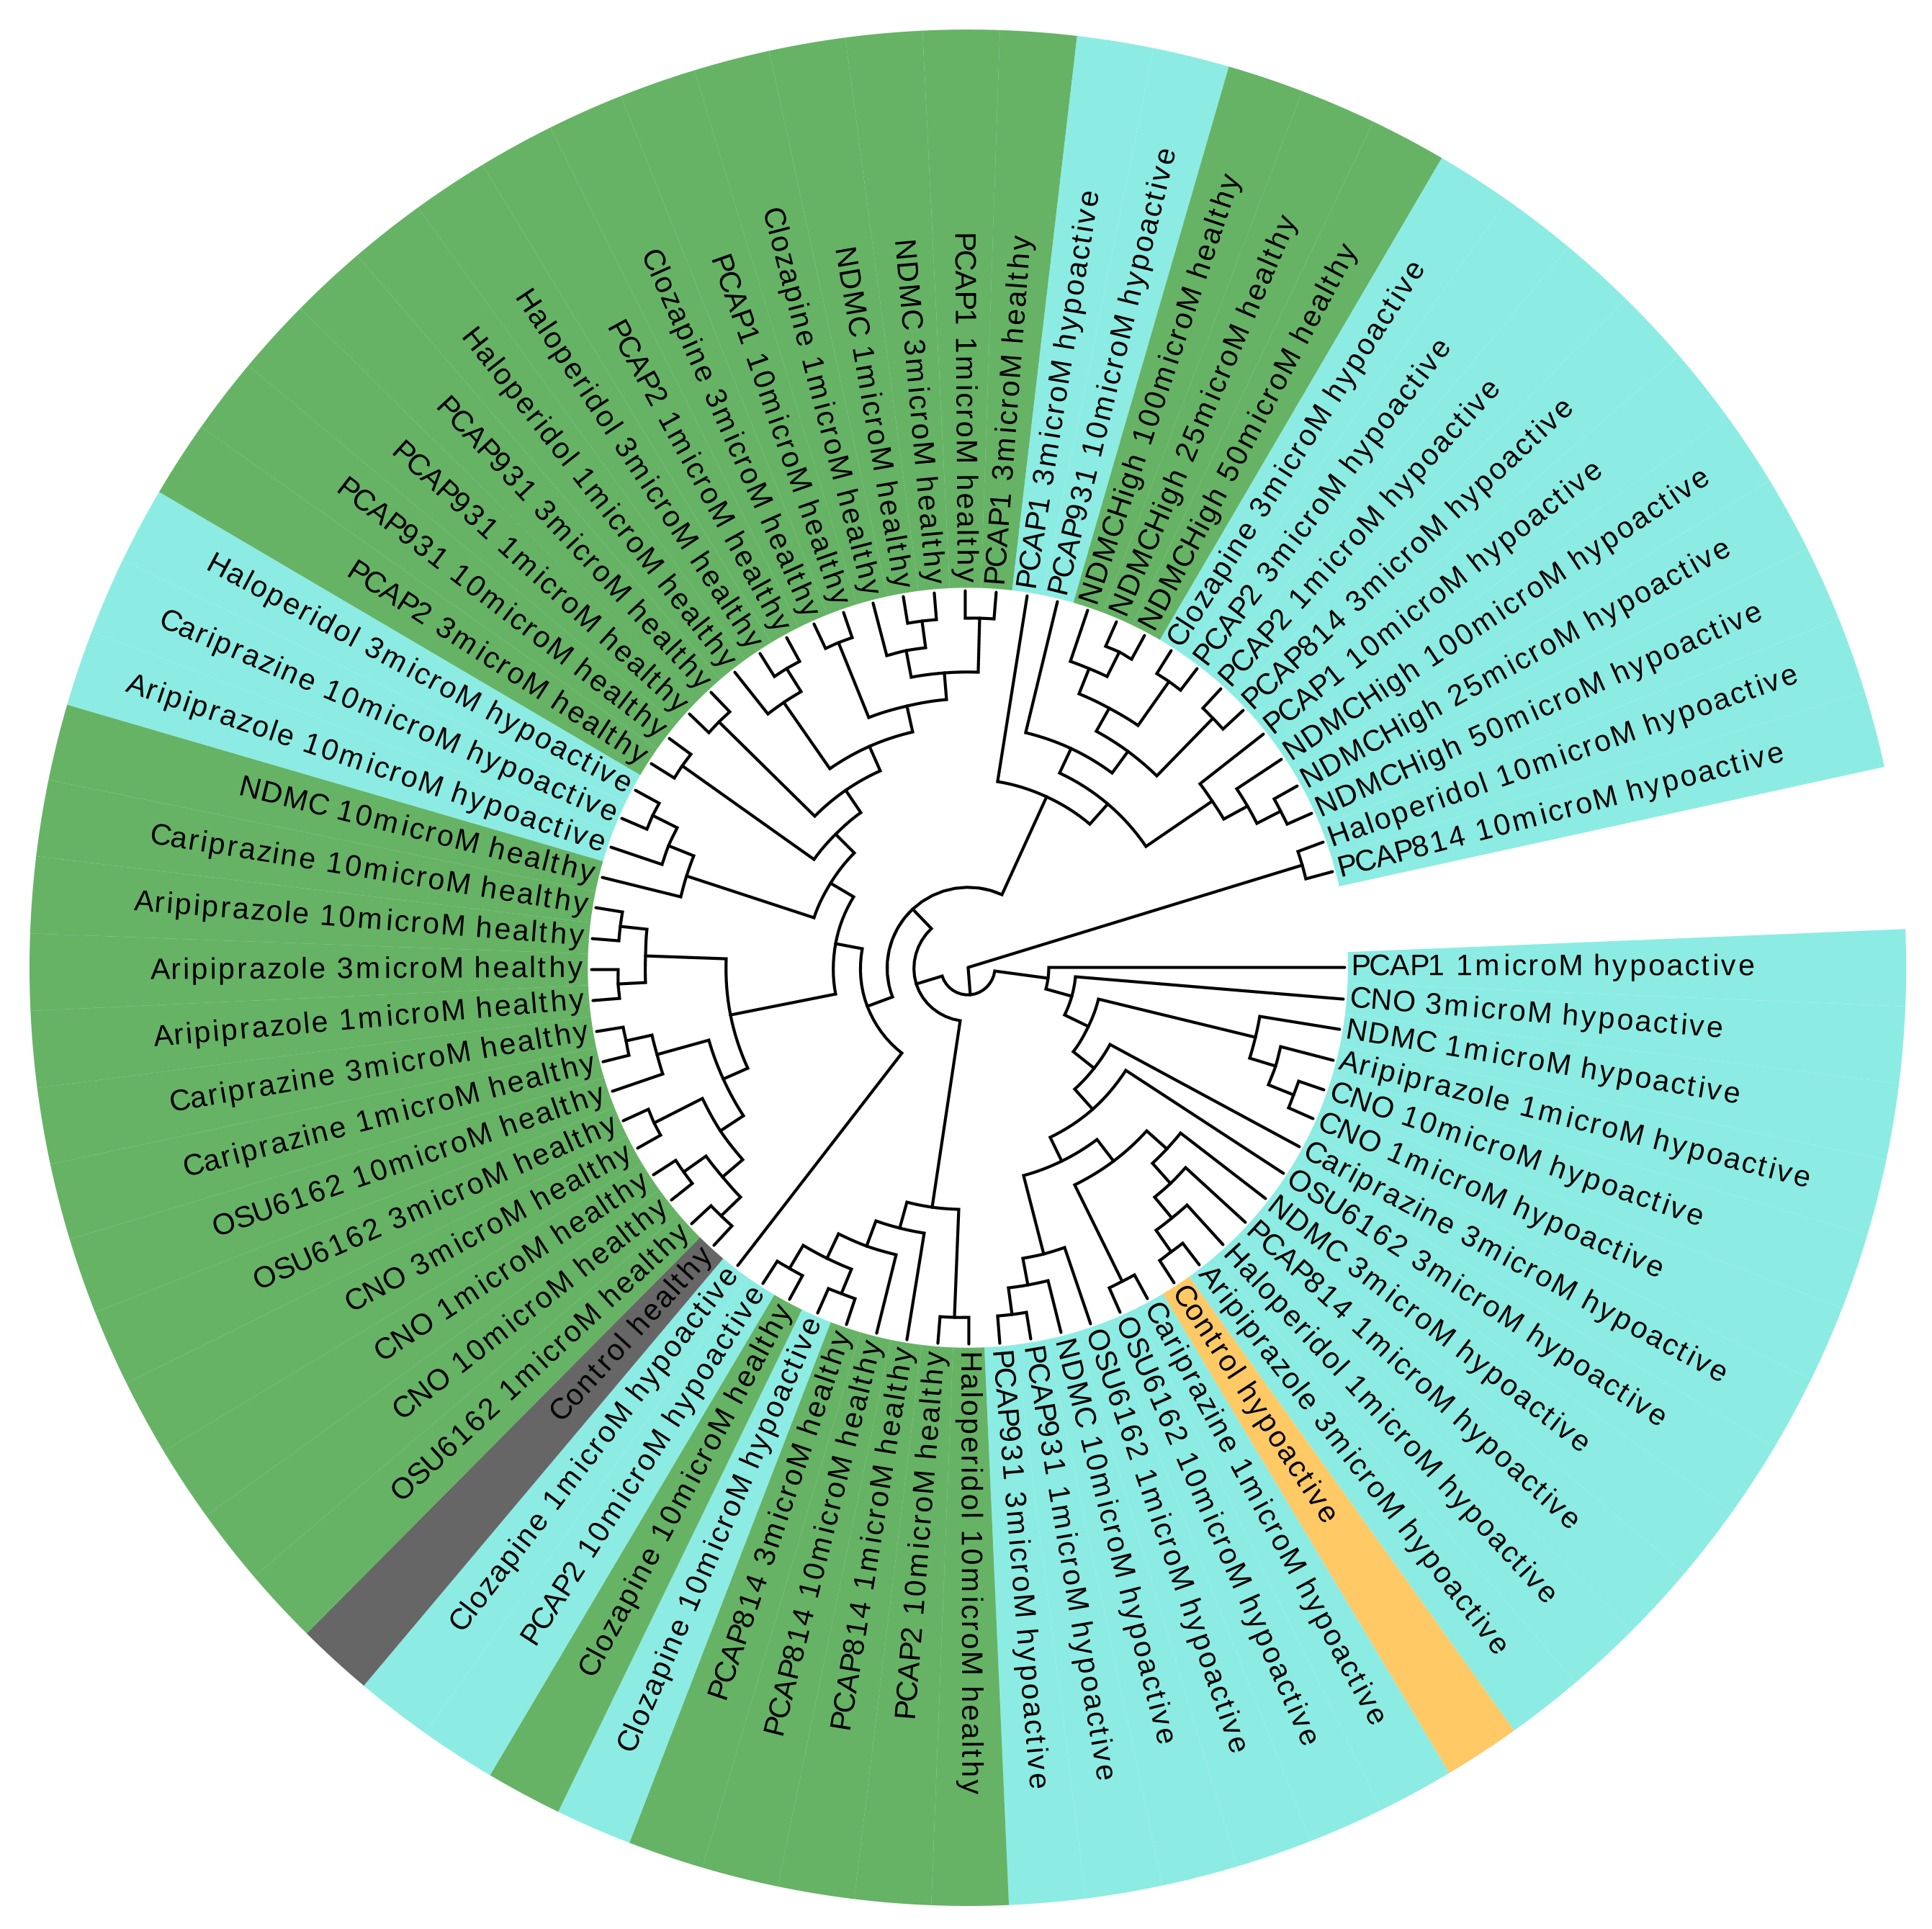
\includegraphics[width=8cm,height=7.5cm]{DarkApoLow_set1_PCA_tree.png}
\caption{Circular cladogram, representing Euclidean distances between the first five principal components of all experimental groups in the healthy and hypoactive condition, using the first set of descriptive statistics.}
\end{center}
\end{figure}
\begin{figure}[h!]
\begin{center}
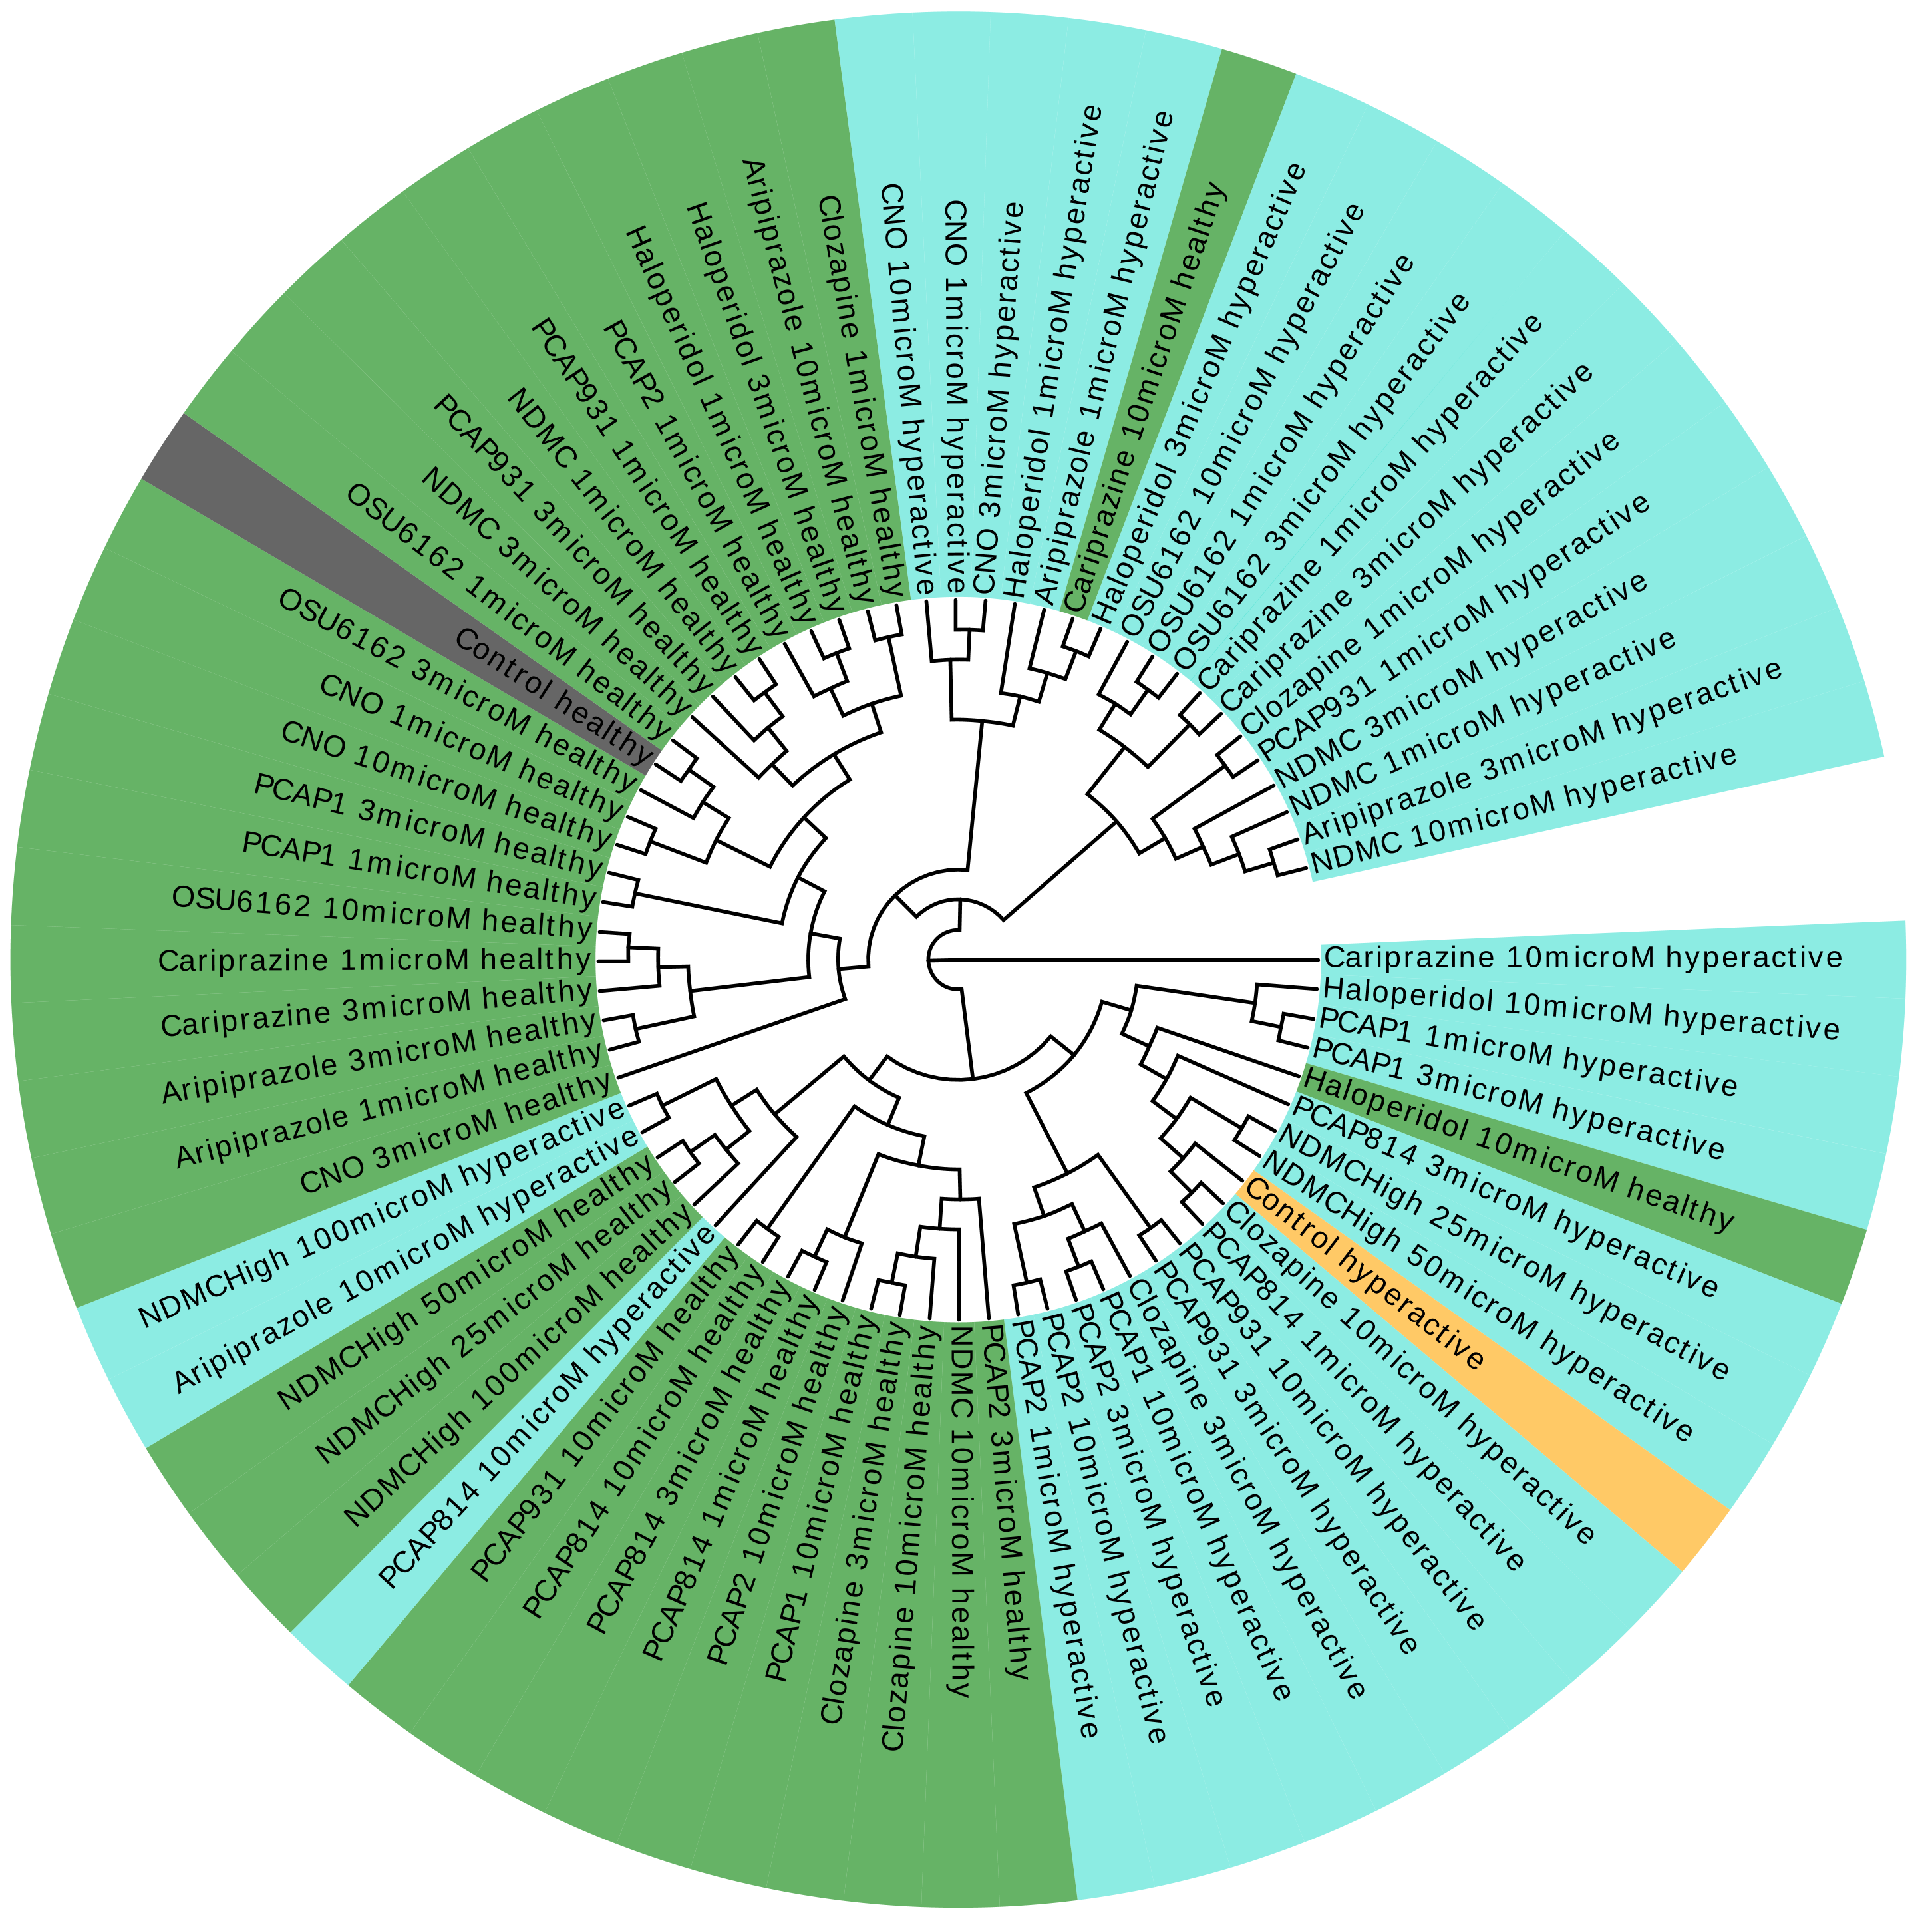
\includegraphics[width=8cm,height=7.5cm]{DarkApoHigh_set1_PCA_tree.png}
\caption{Circular cladogram, representing Euclidean distances between the first five principal components of all experimental groups in the healthy and type I hyperactive condition, using the first set of descriptive statistics.}
\end{center}
\end{figure}
\begin{figure}[h!]
\begin{center}
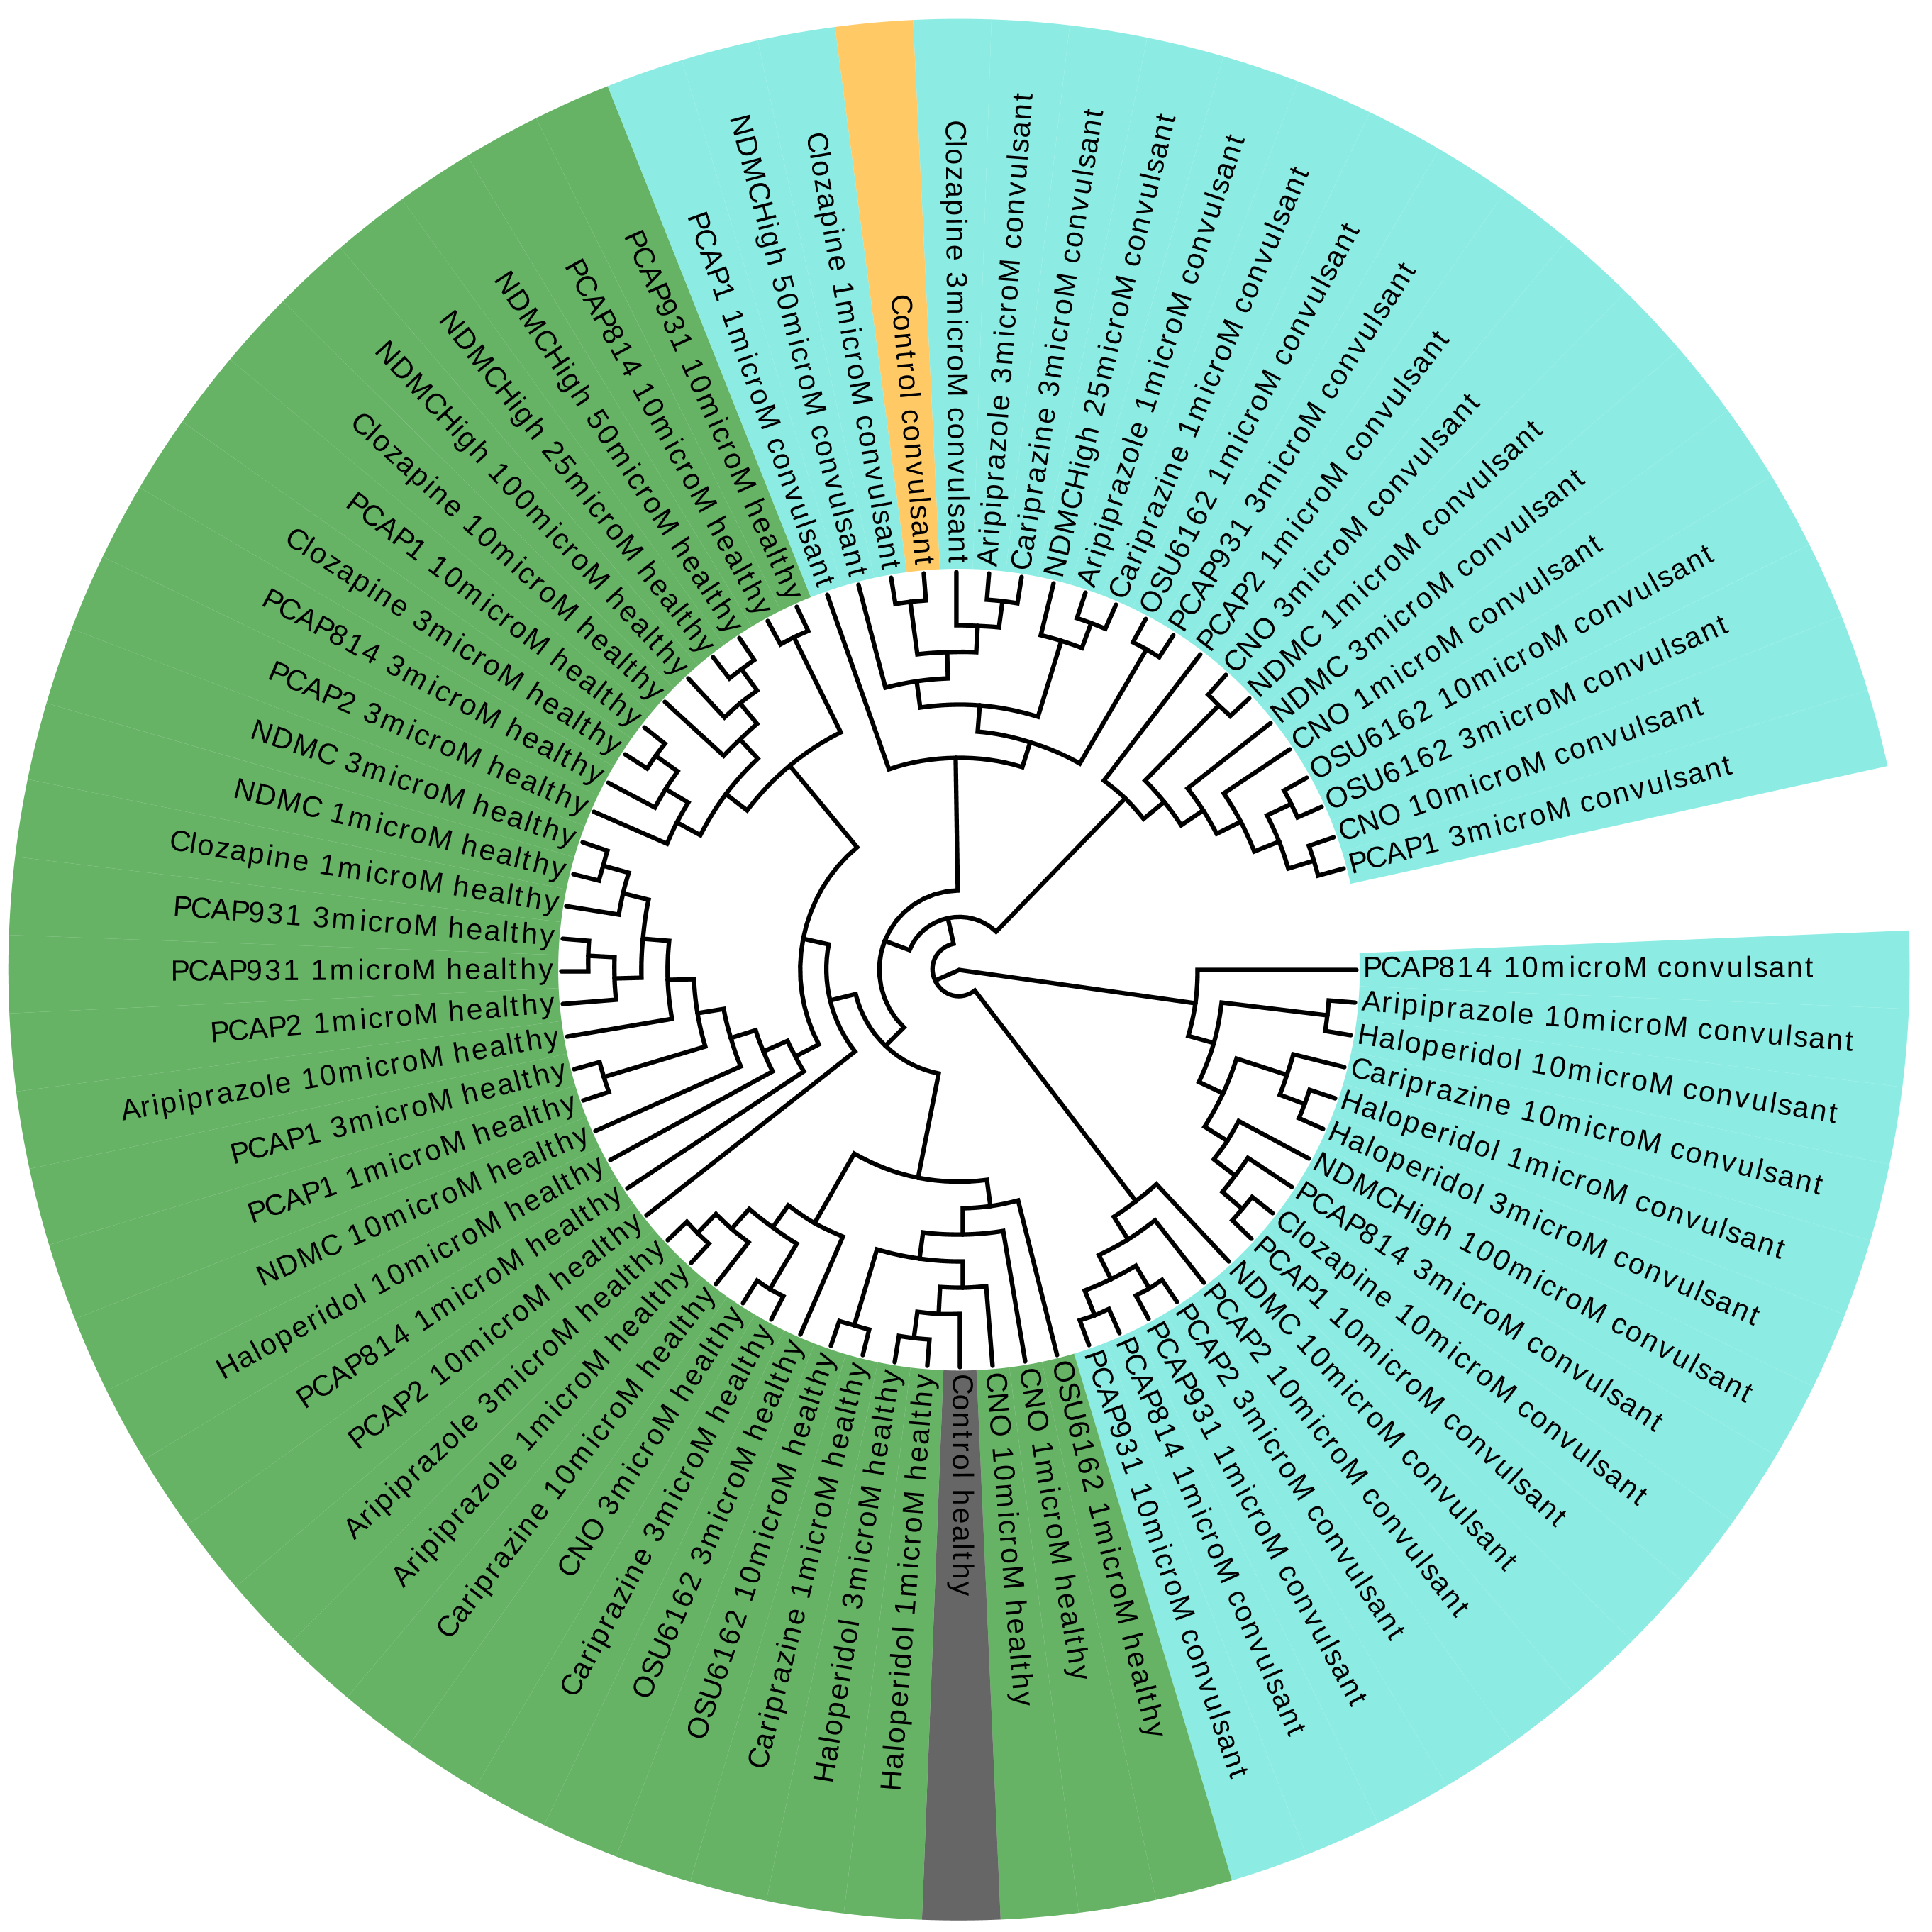
\includegraphics[width=8cm,height=7.5cm]{DarkPTZ_set1_PCA_tree.png}
\caption{Circular cladogram, representing Euclidean distances between the first five principal components of all experimental groups in the healthy and type II hyperactive condition, using the first set of descriptive statistics.}
\end{center}
\end{figure}
\begin{figure}[h!]
\begin{center}
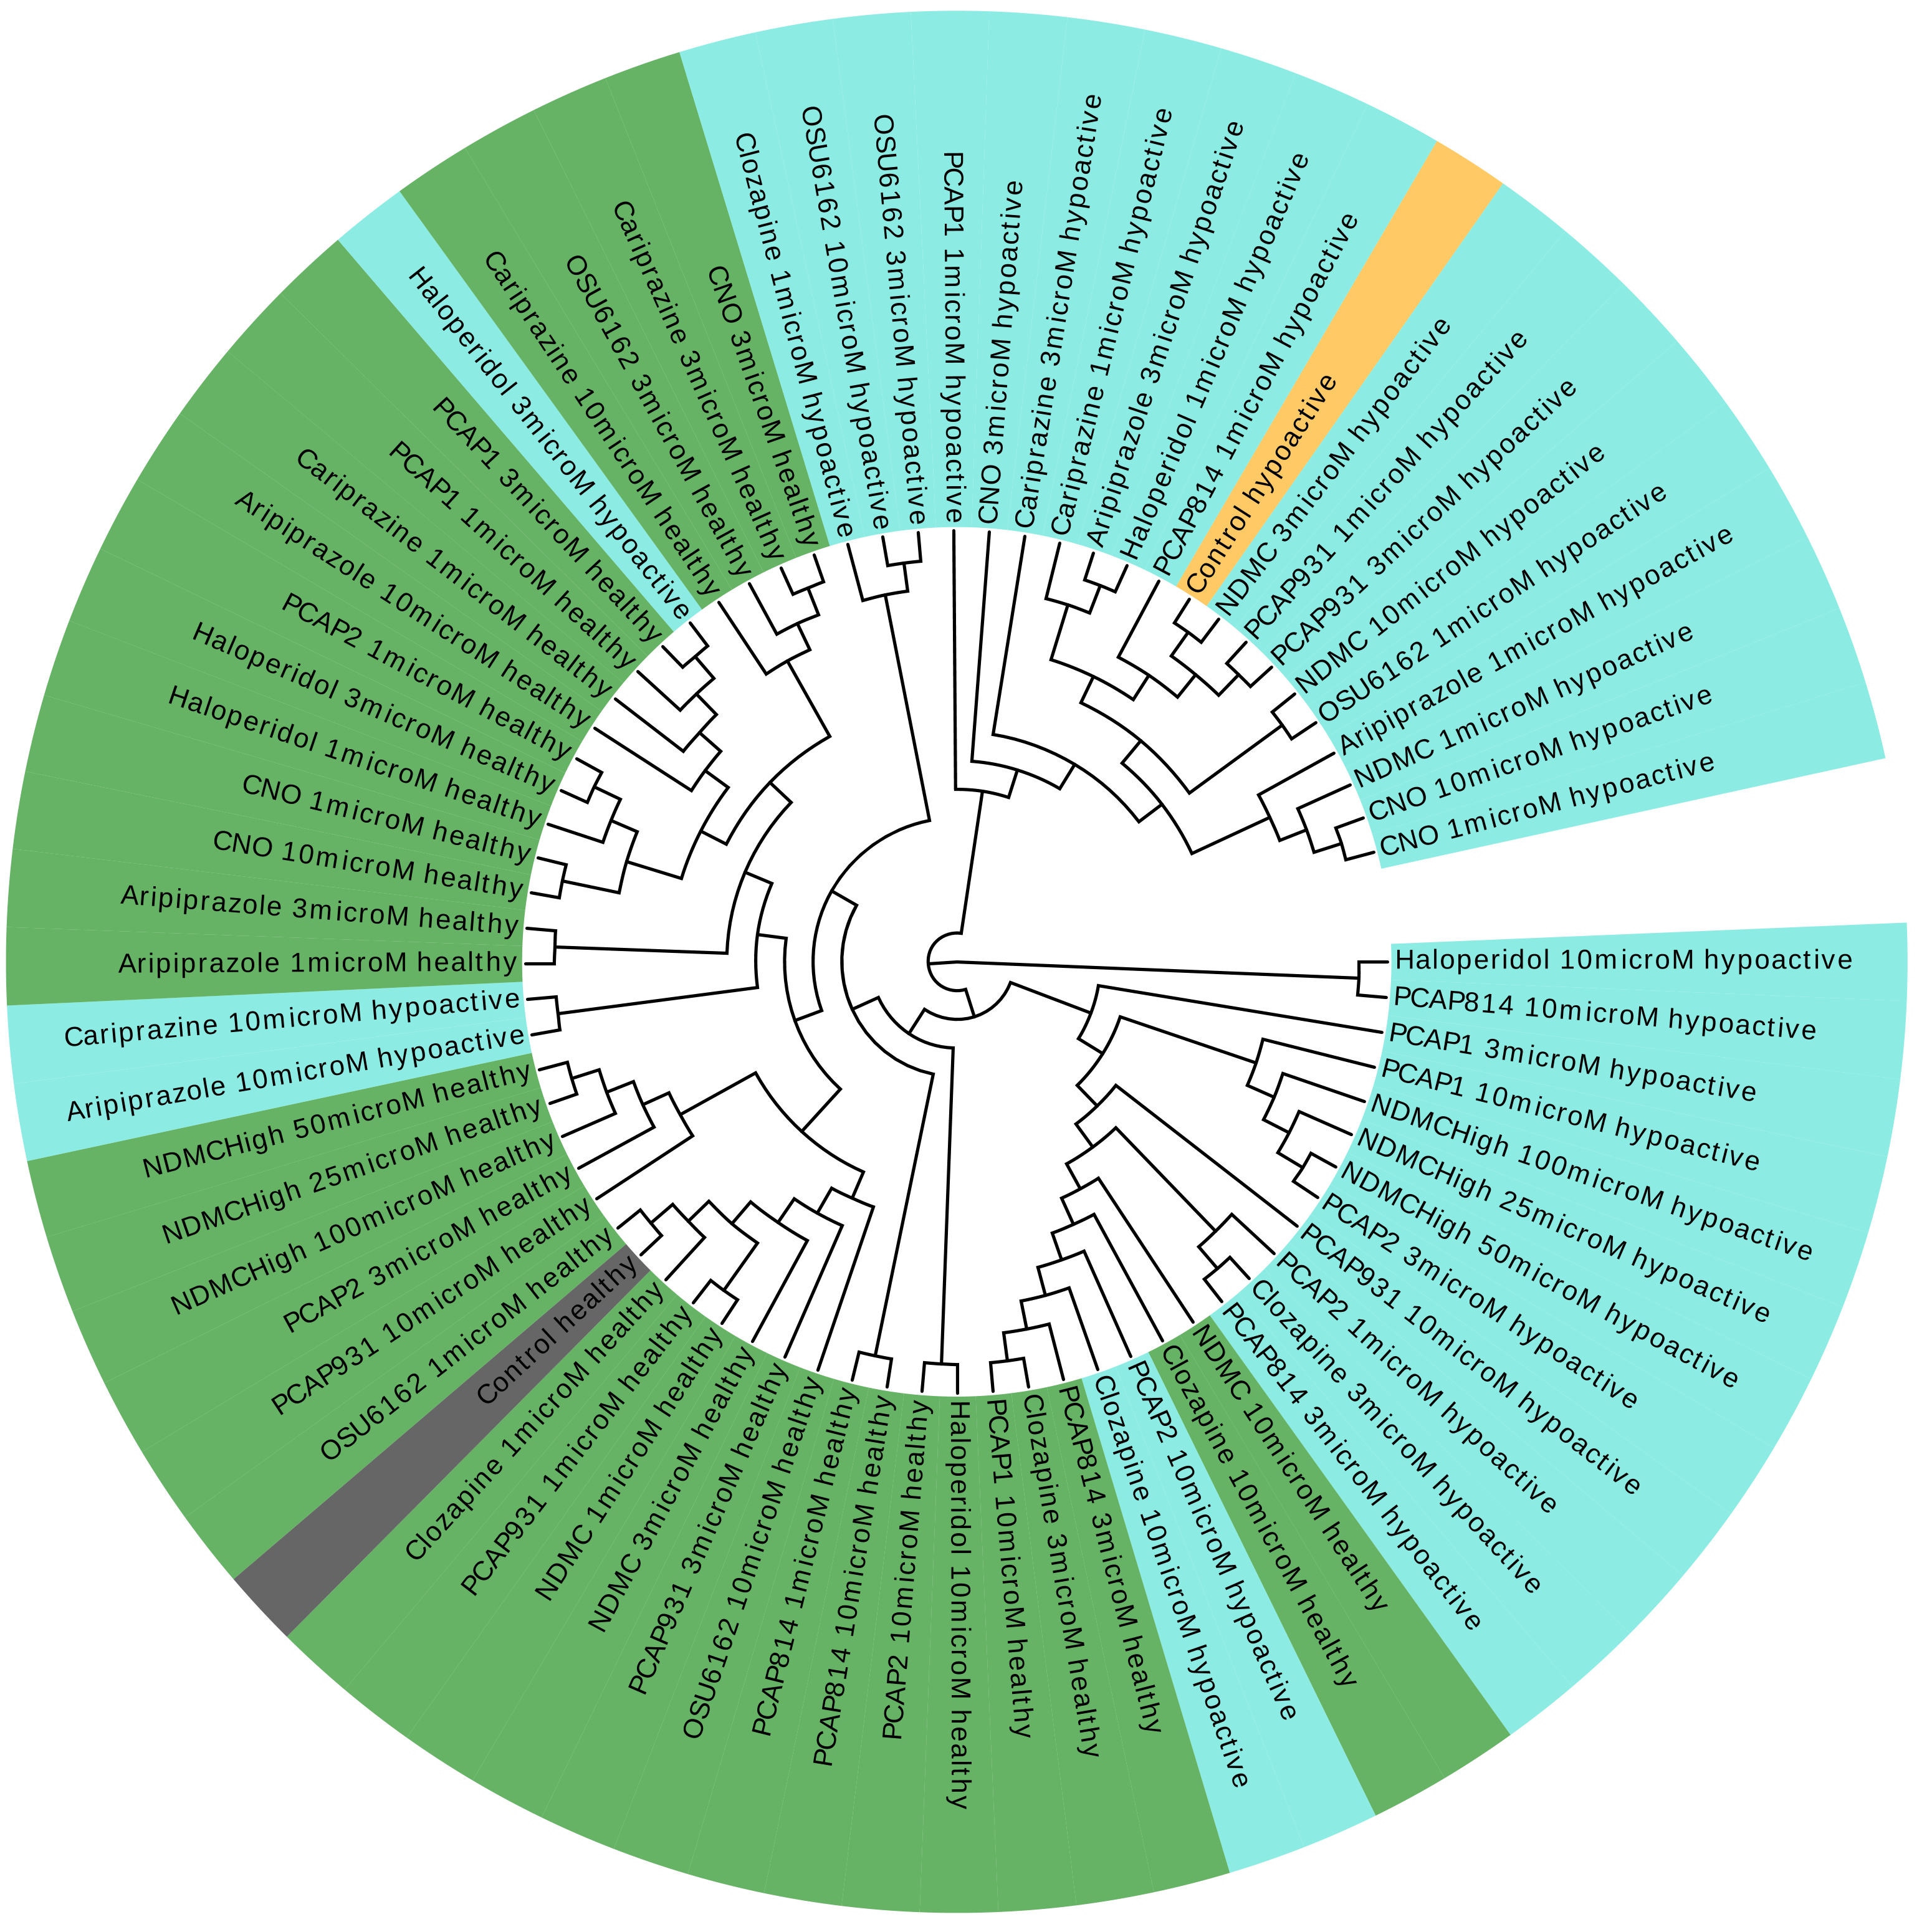
\includegraphics[width=8cm,height=7.5cm]{DarkApoLow_set2_PCA_tree.png}
\caption{Circular cladogram, representing Euclidean distances between the first five principal components of all experimental groups in the healthy and hypoactive condition, using the second set of descriptive statistics.}
\end{center}
\end{figure}
\begin{figure}[h!]
\begin{center}
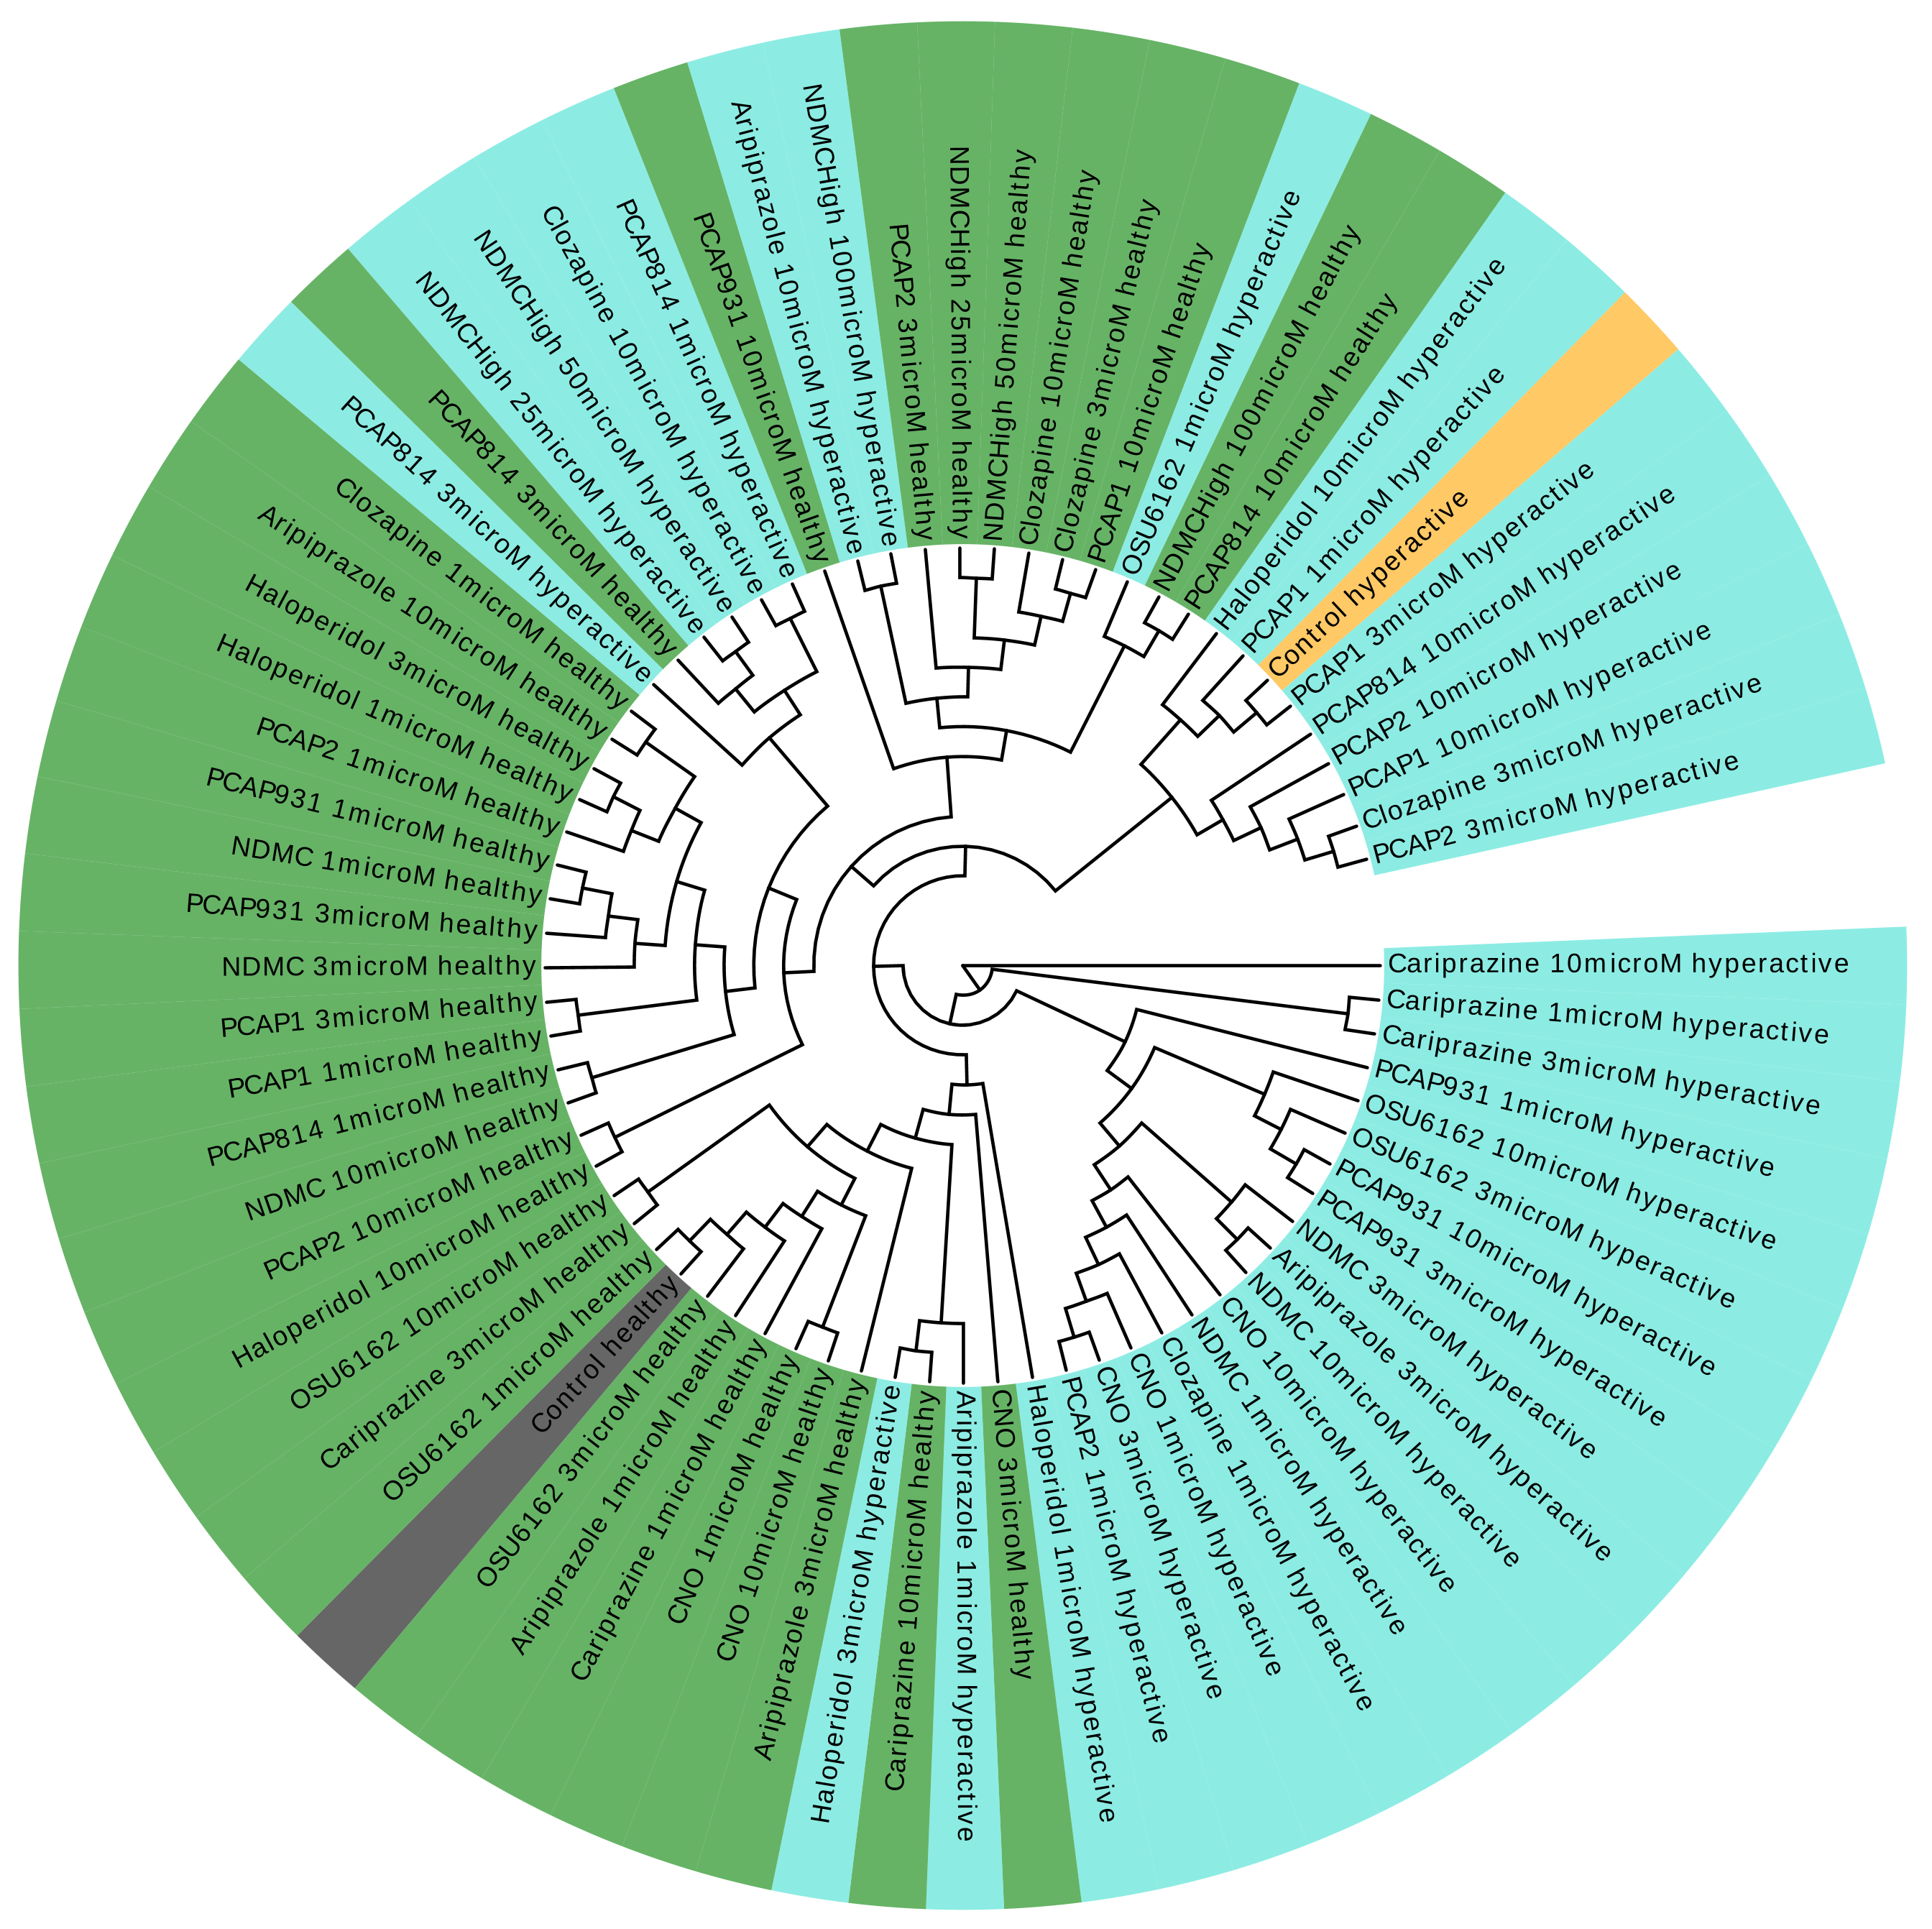
\includegraphics[width=8cm,height=7.5cm]{DarkApoHigh_set2_PCA_tree.png}
\caption{Circular cladogram, representing Euclidean distances between the first five principal components of all experimental groups in the healthy and type I hyperactive condition, using the second set of descriptive statistics.}
\end{center}
\end{figure}
\begin{figure}[h!]
\begin{center}
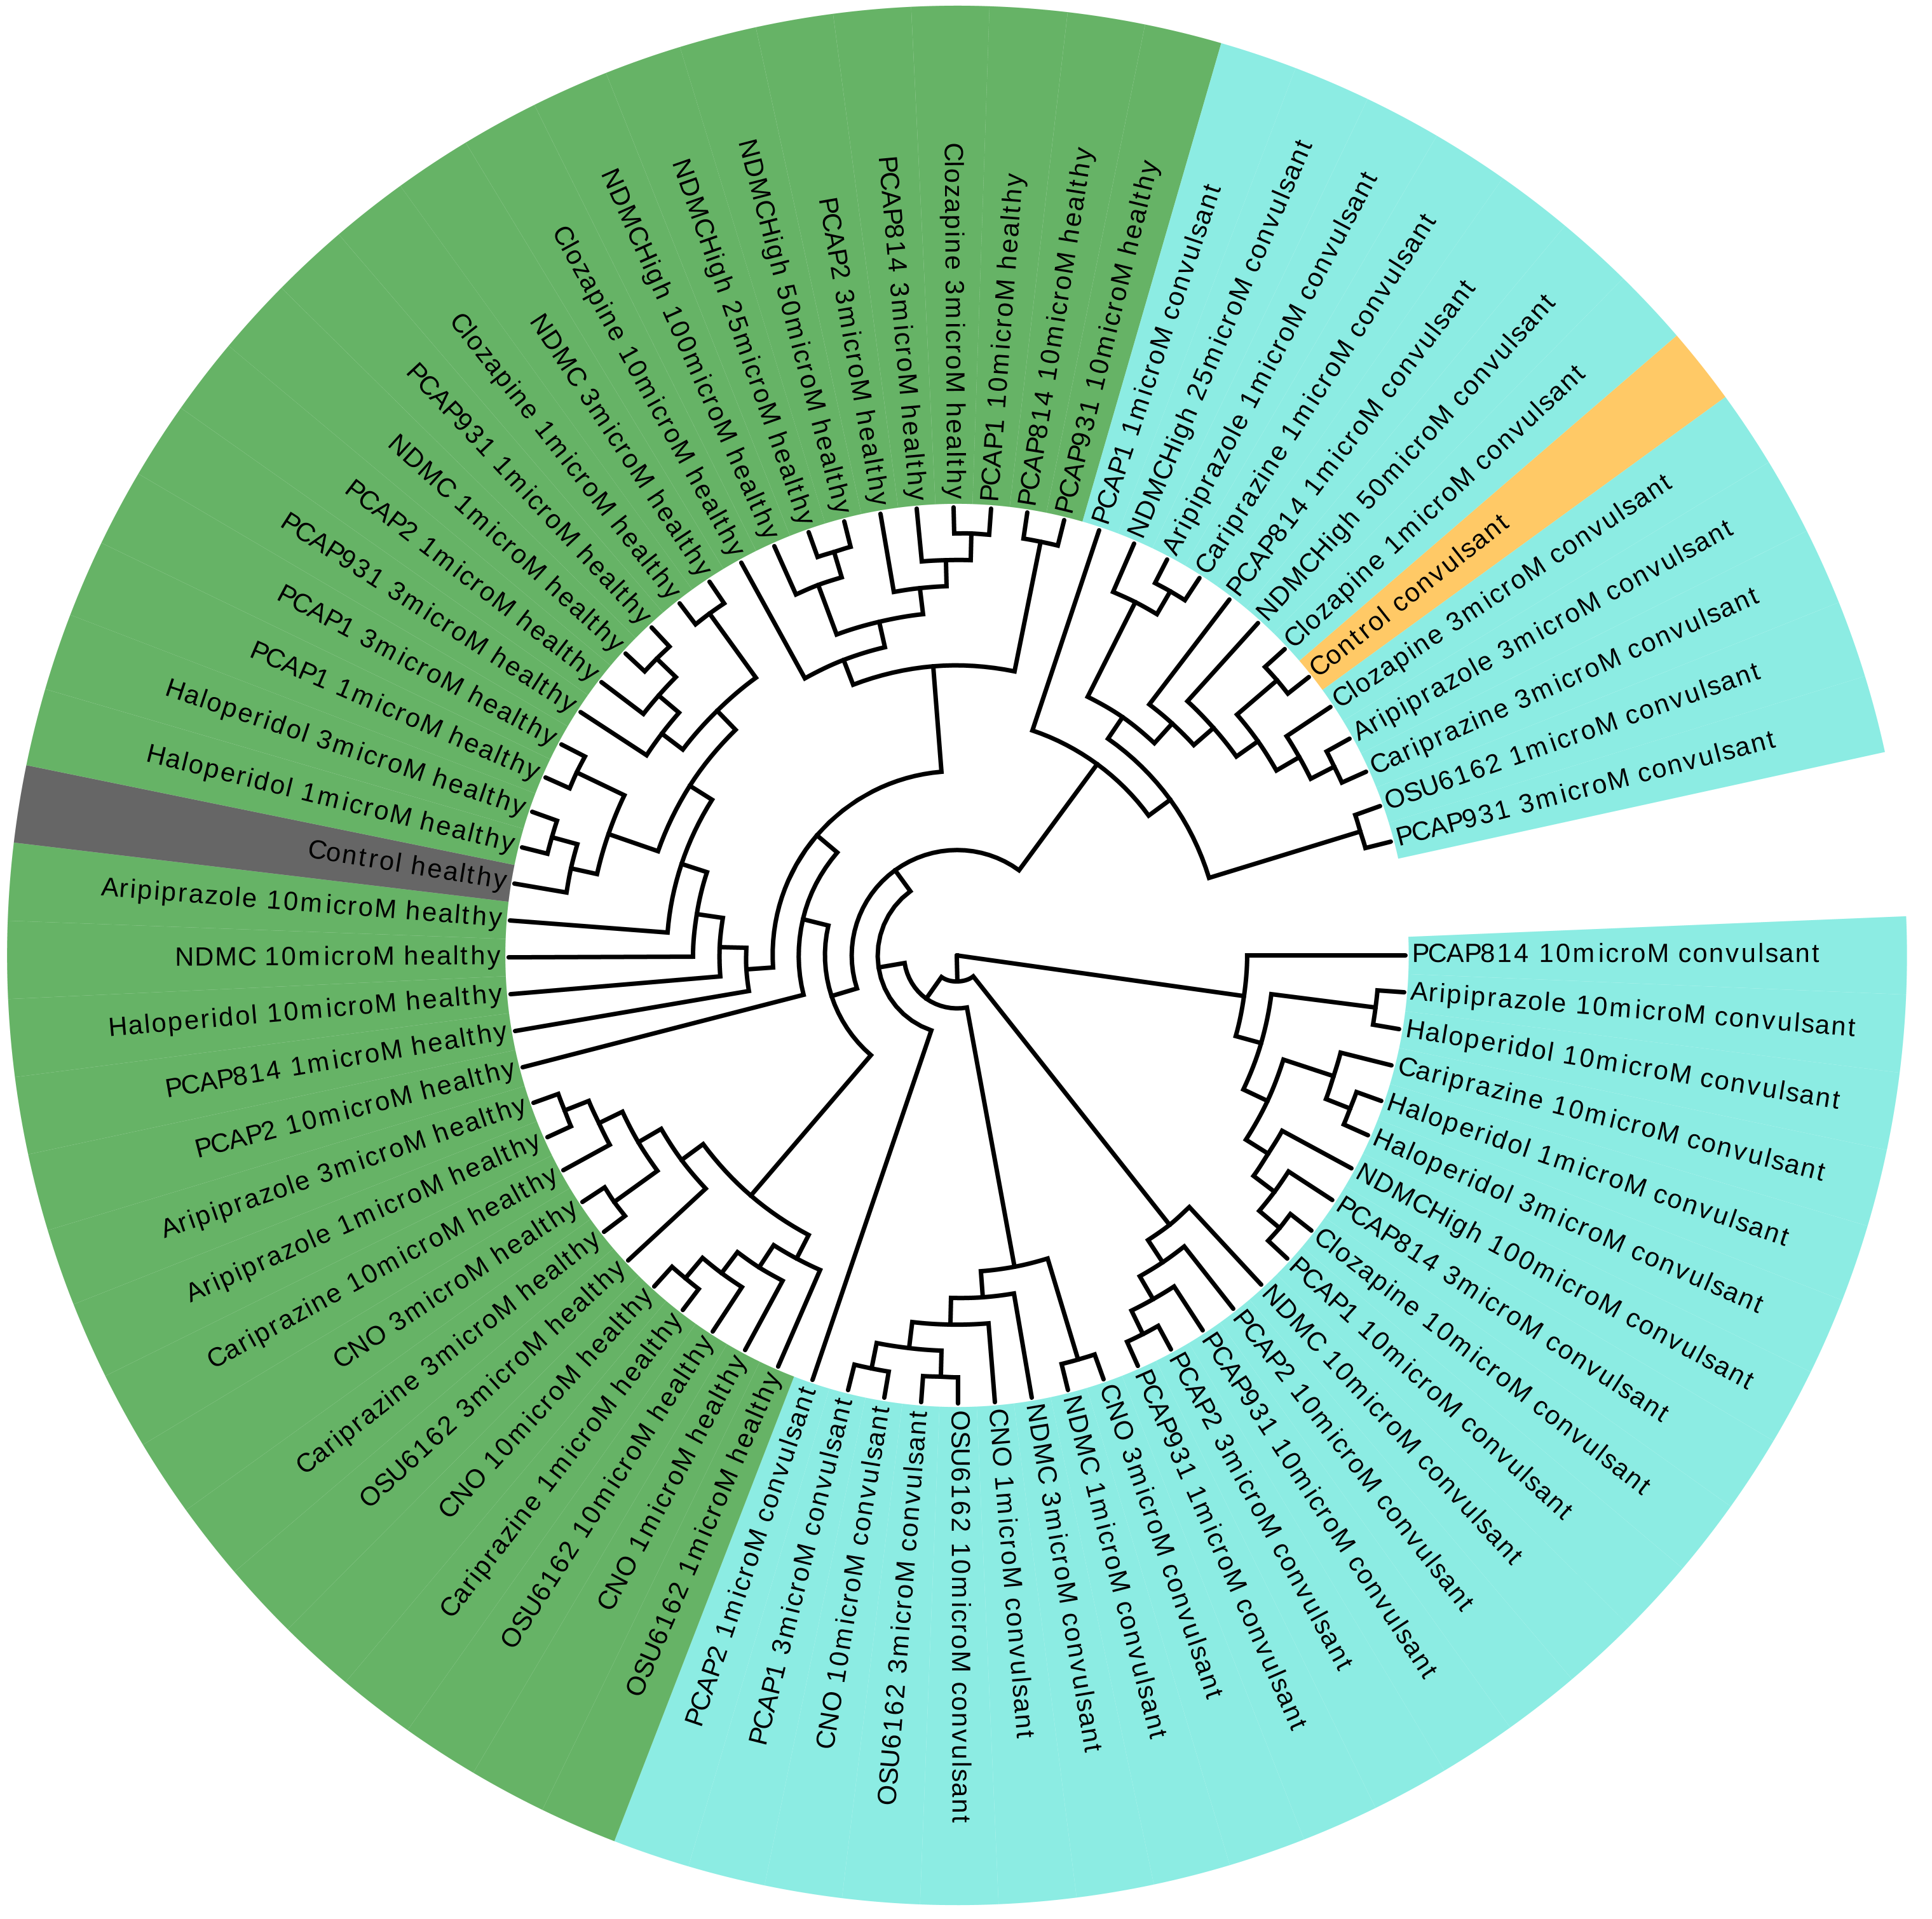
\includegraphics[width=8cm,height=7.5cm]{DarkPTZ_set2_PCA_tree.png}
\caption{Circular cladogram, representing Euclidean distances between the first five principal components of all experimental groups in the healthy and type II hyperactive condition, using the second set of descriptive statistics.}
\end{center}
\end{figure}
\begin{figure}[h!]
\begin{center}
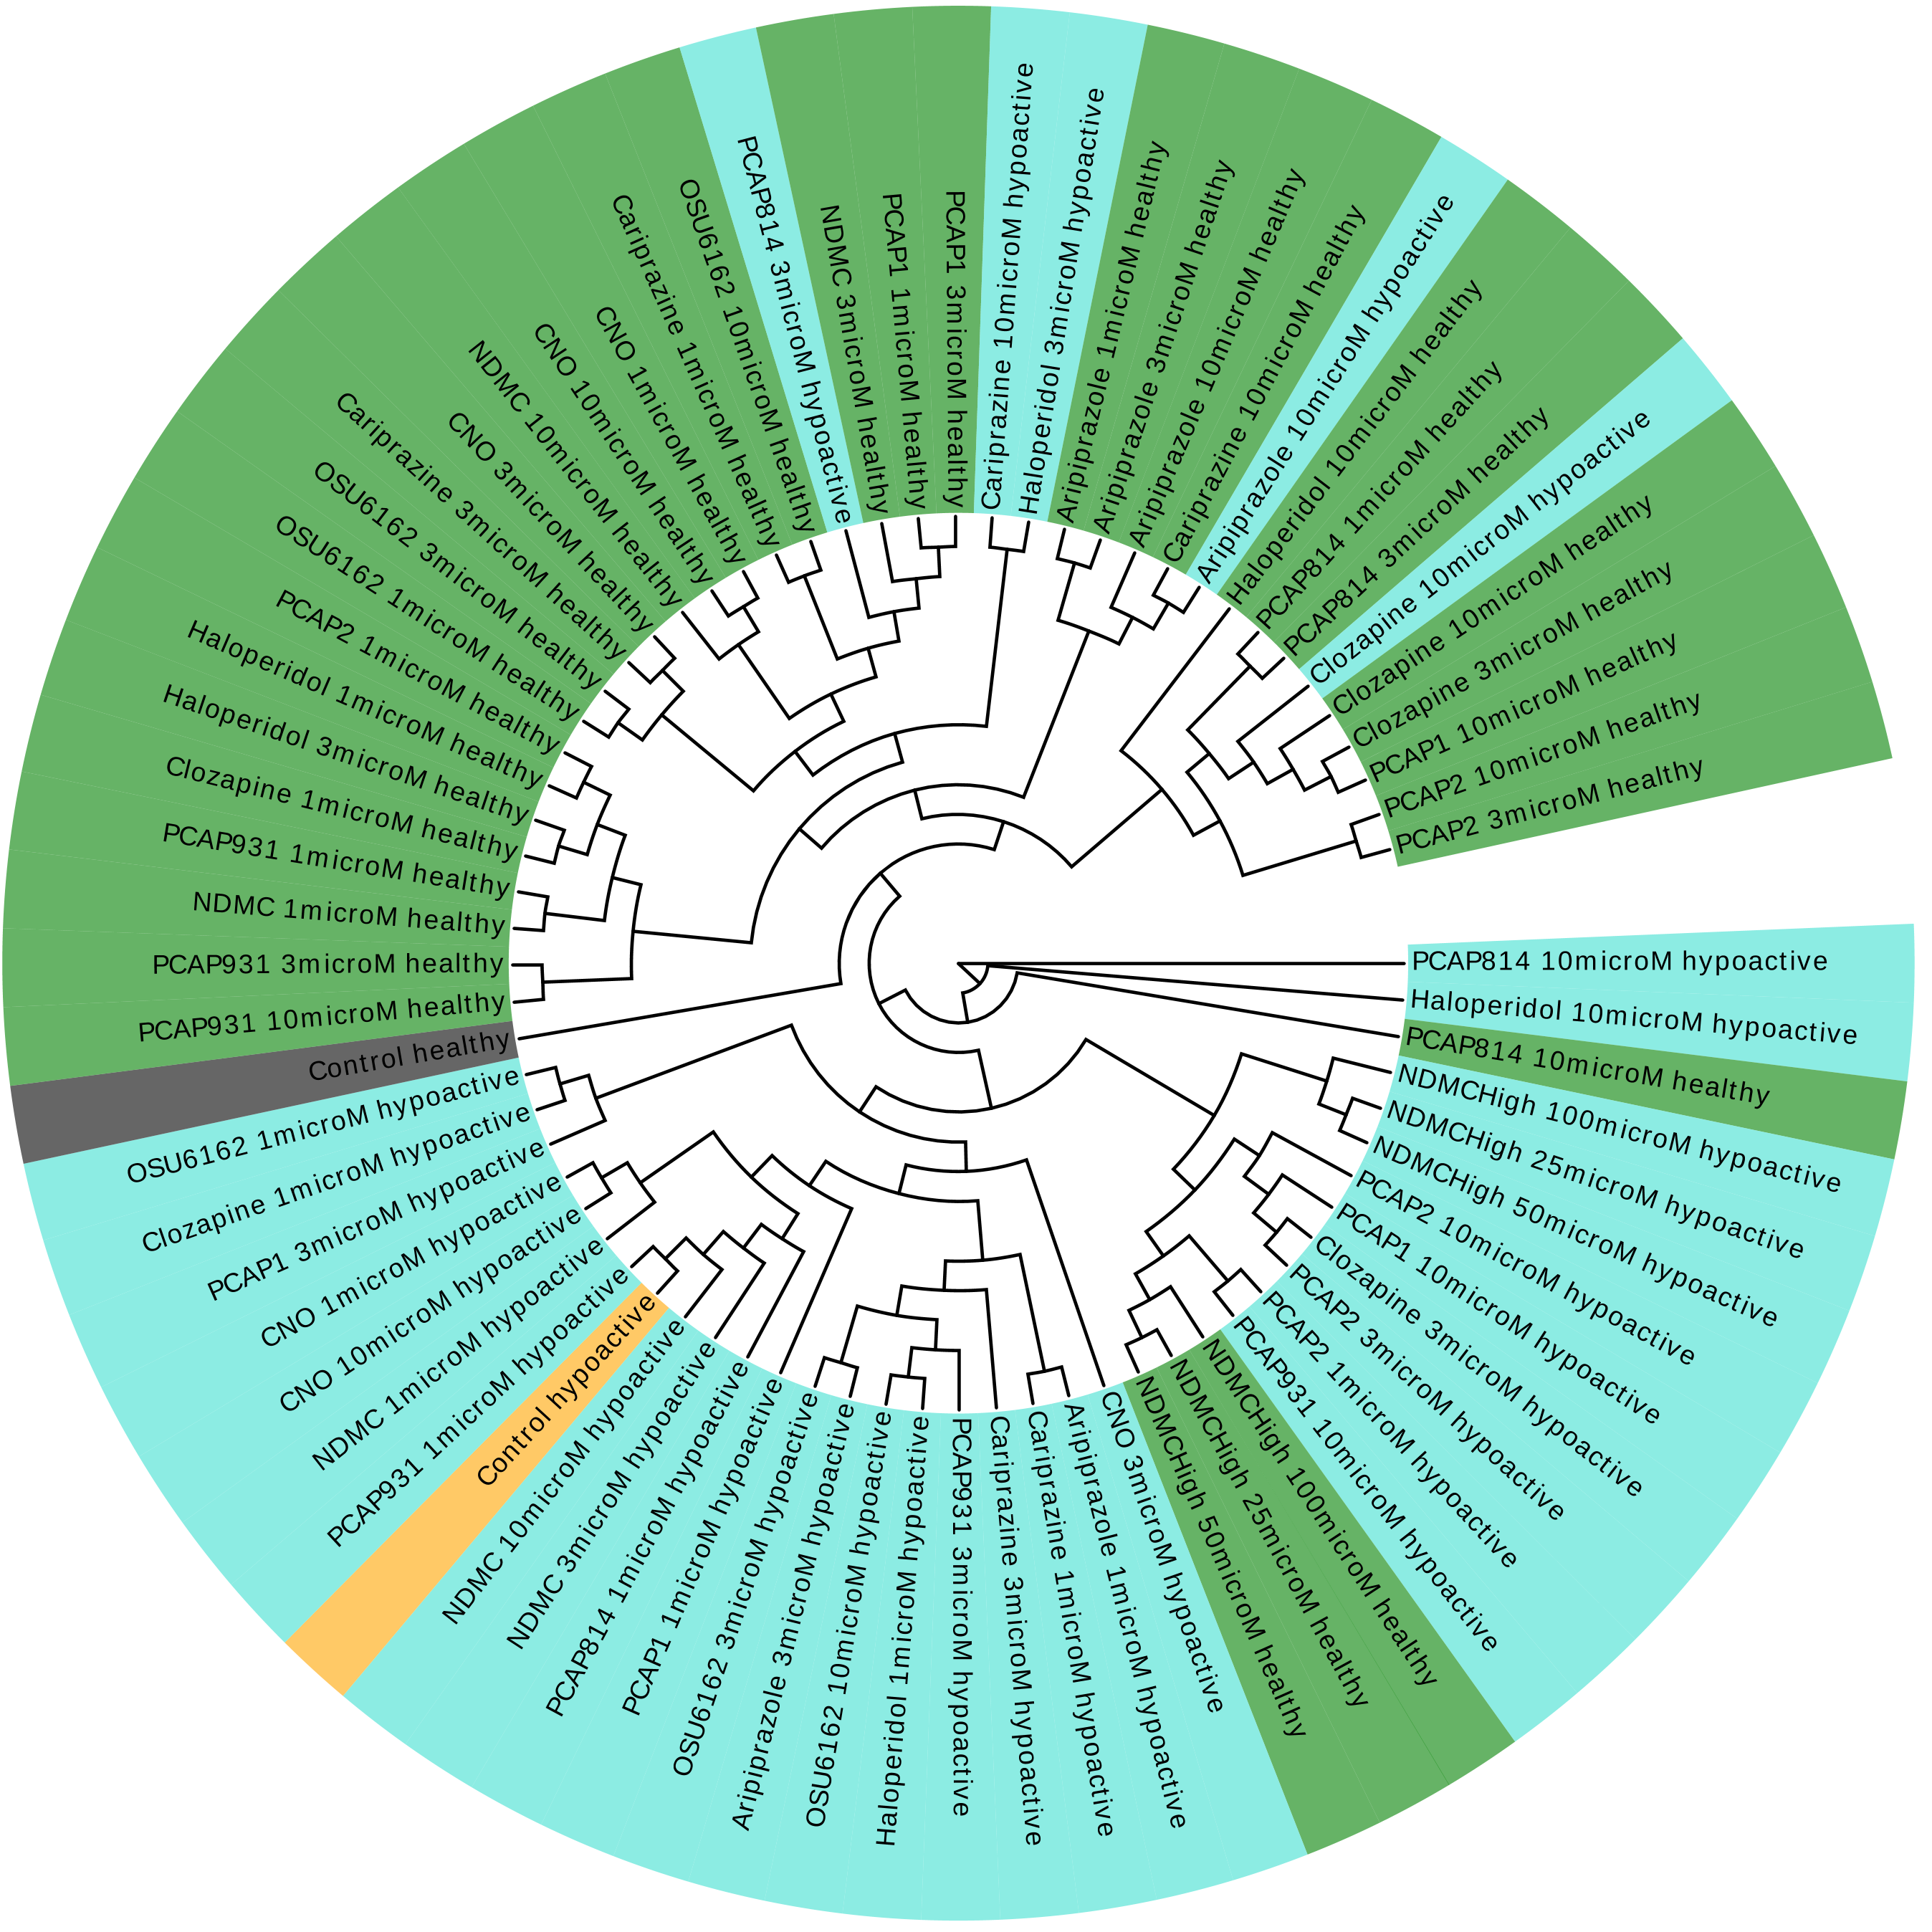
\includegraphics[width=8cm,height=7.5cm]{DarkApoLow_set3_PCA_tree.png}
\caption{Circular cladogram, representing Euclidean distances between the first five principal components of all experimental groups in the healthy and hypoactive condition, using the third set of descriptive statistics.}
\end{center}
\end{figure}
\begin{figure}[h!]
\begin{center}
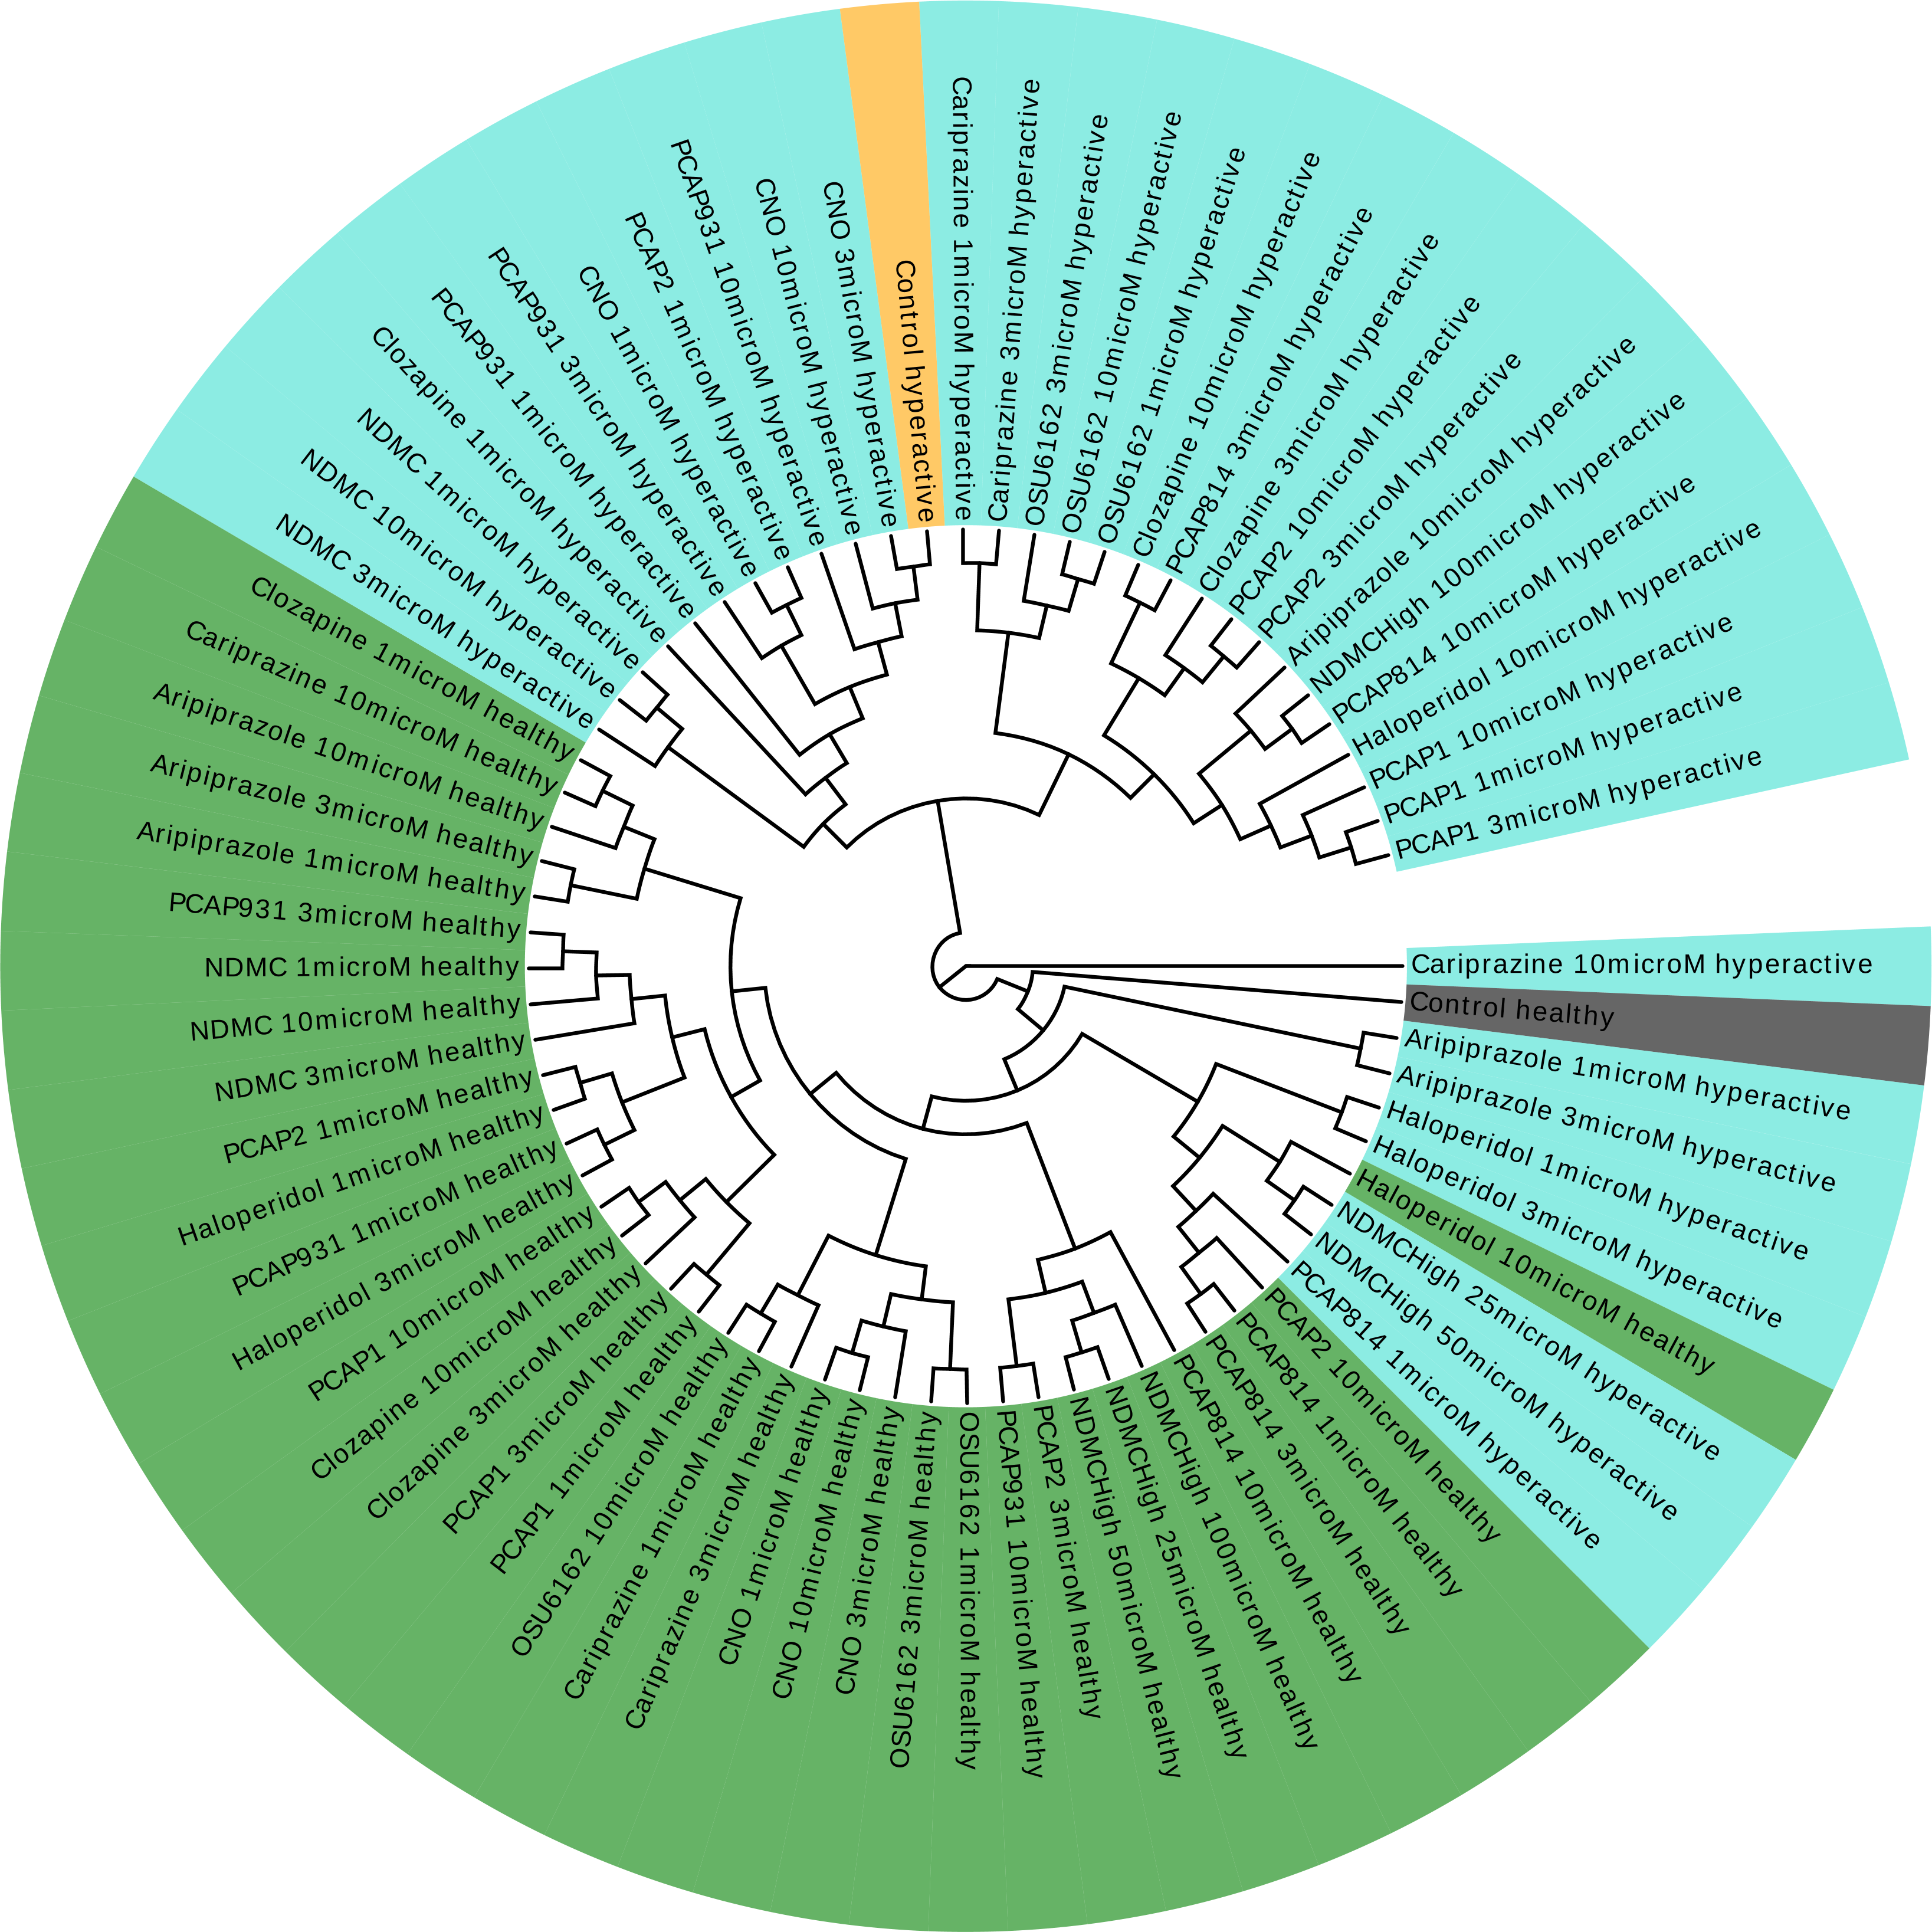
\includegraphics[width=8cm,height=7.5cm]{DarkApoHigh_set3_PCA_tree.png}
\caption{Circular cladogram, representing Euclidean distances between the first five principal components of all experimental groups in the healthy and type I hyperactive condition, using the third set of descriptive statistics.}
\end{center}
\end{figure}
\begin{figure}[h!]
\begin{center}
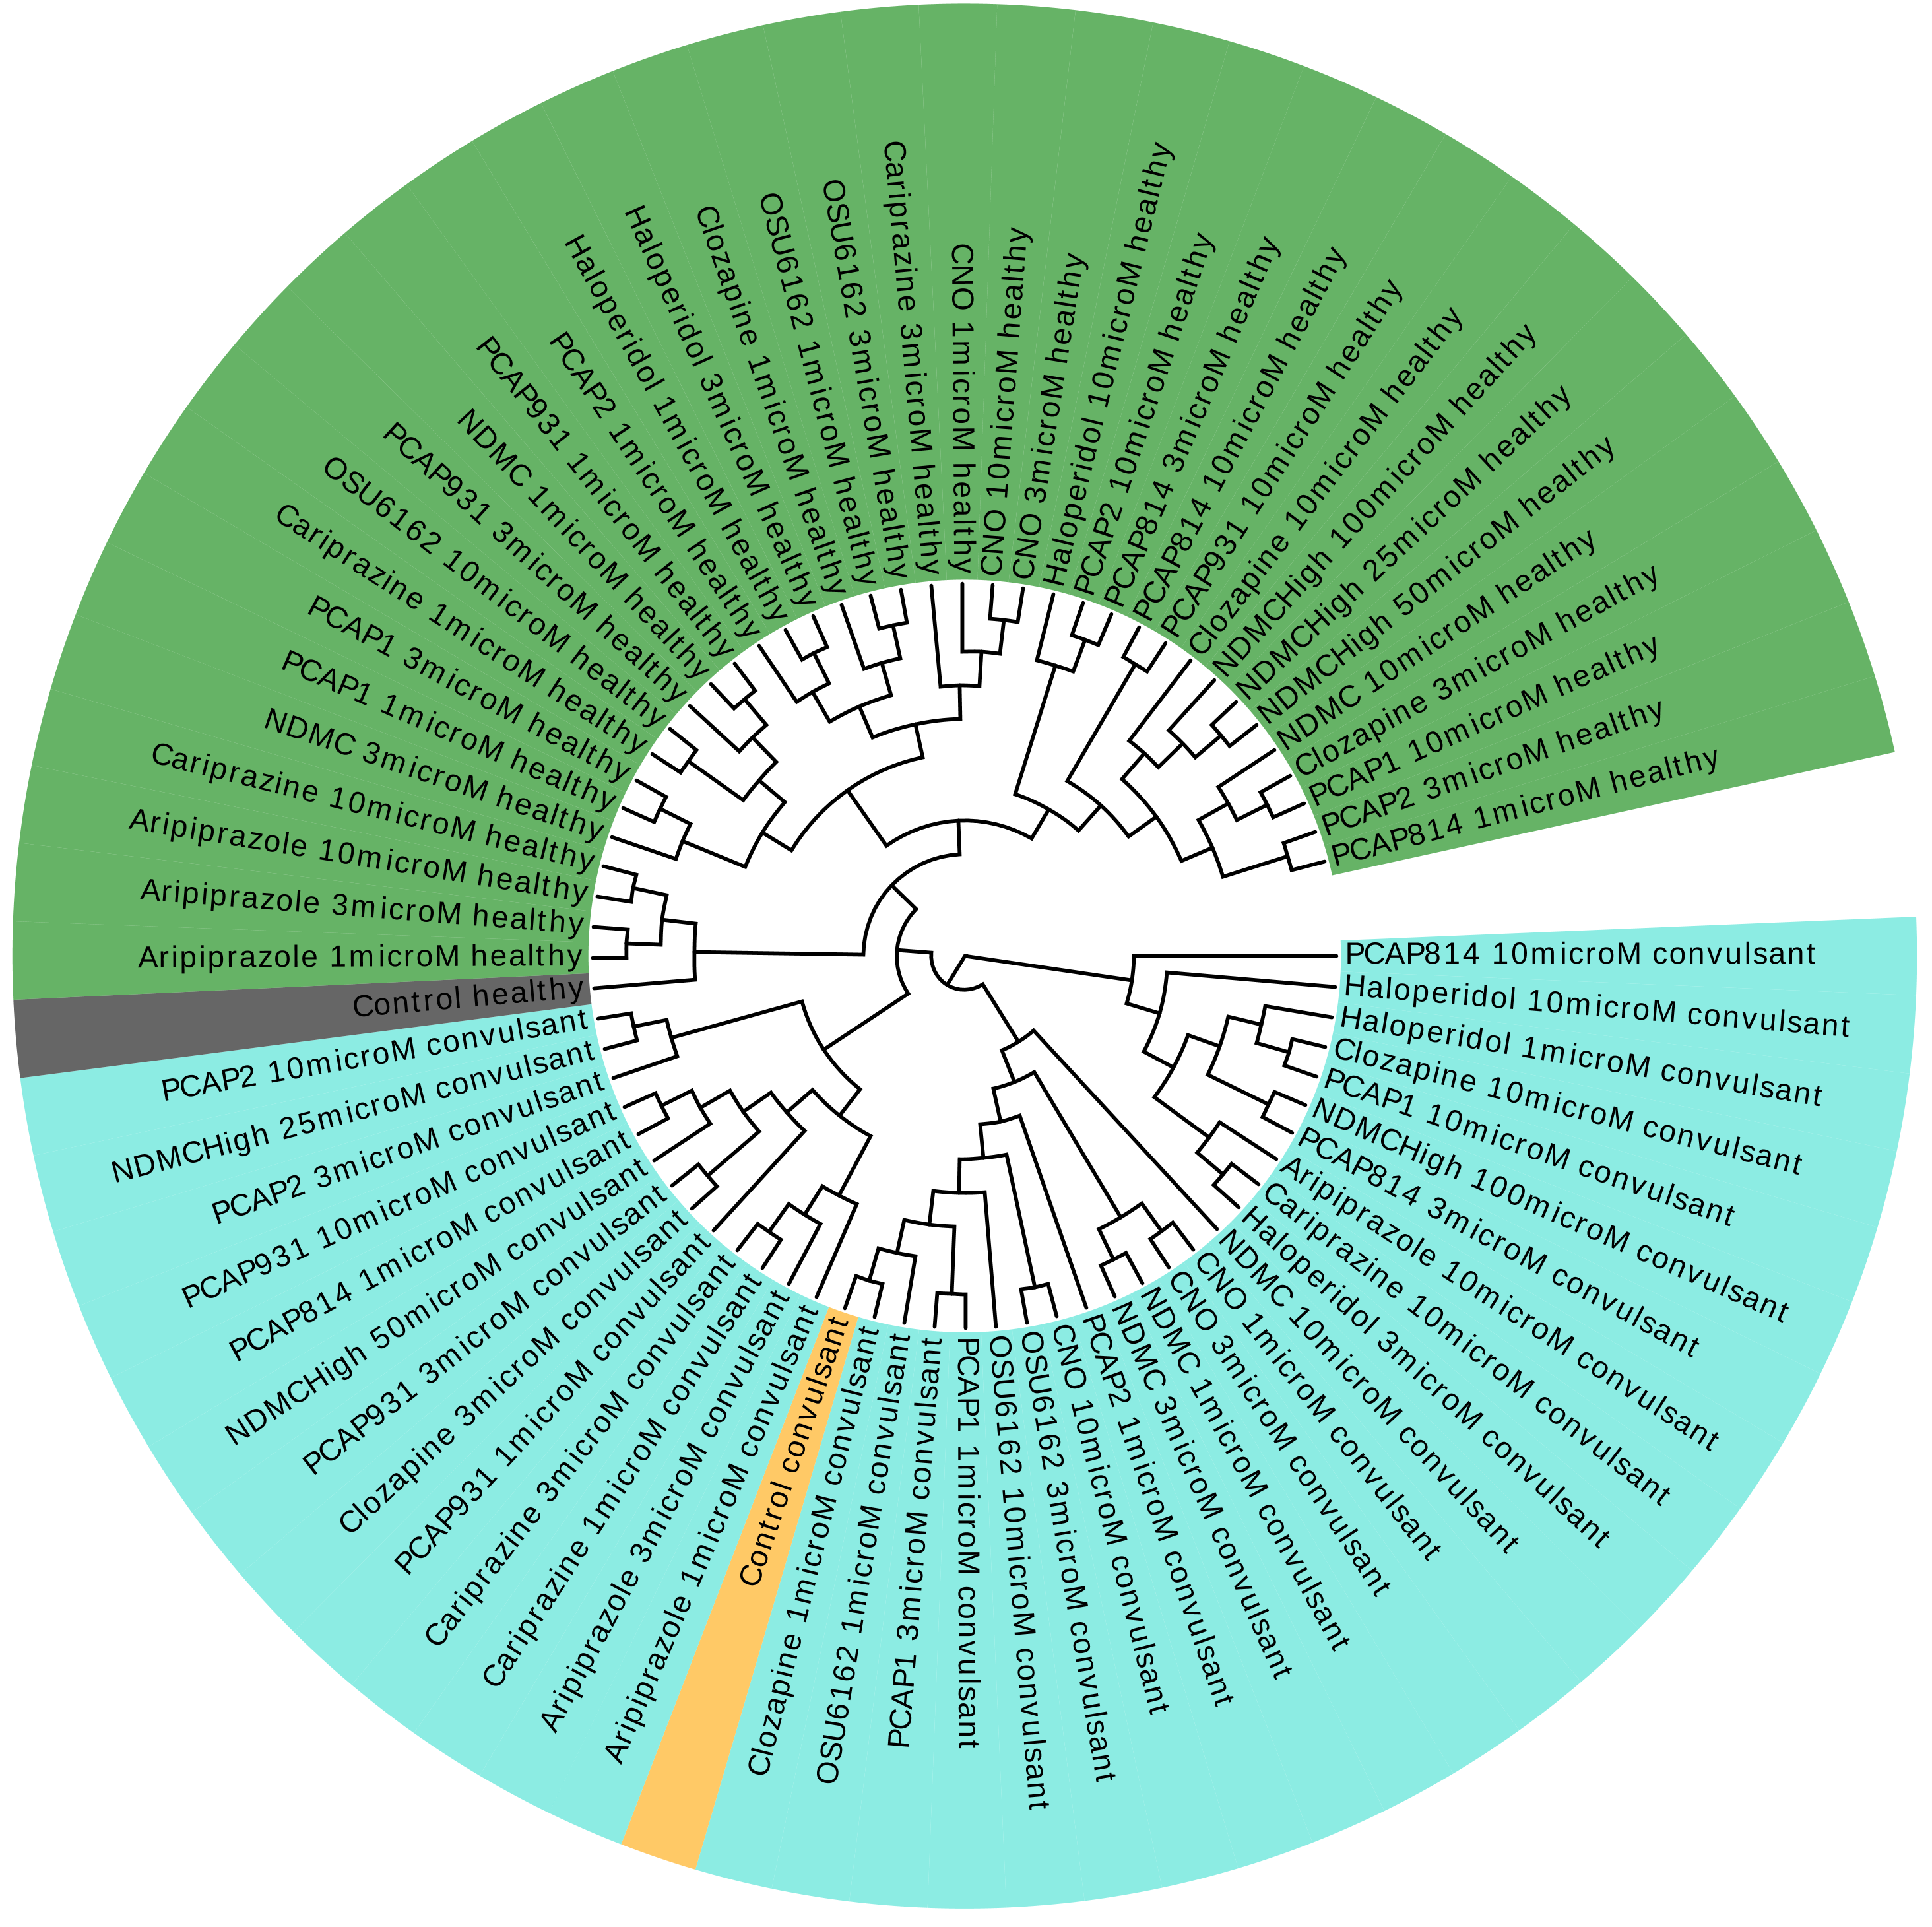
\includegraphics[width=8cm,height=7.5cm]{DarkPTZ_set3_PCA_tree.png}
\caption{Circular cladogram, representing Euclidean distances between the first five principal components of all experimental groups in the healthy and type II hyperactive condition, using the third set of descriptive statistics.}
\end{center}
\end{figure}
\begin{figure}[h!]
\begin{center}
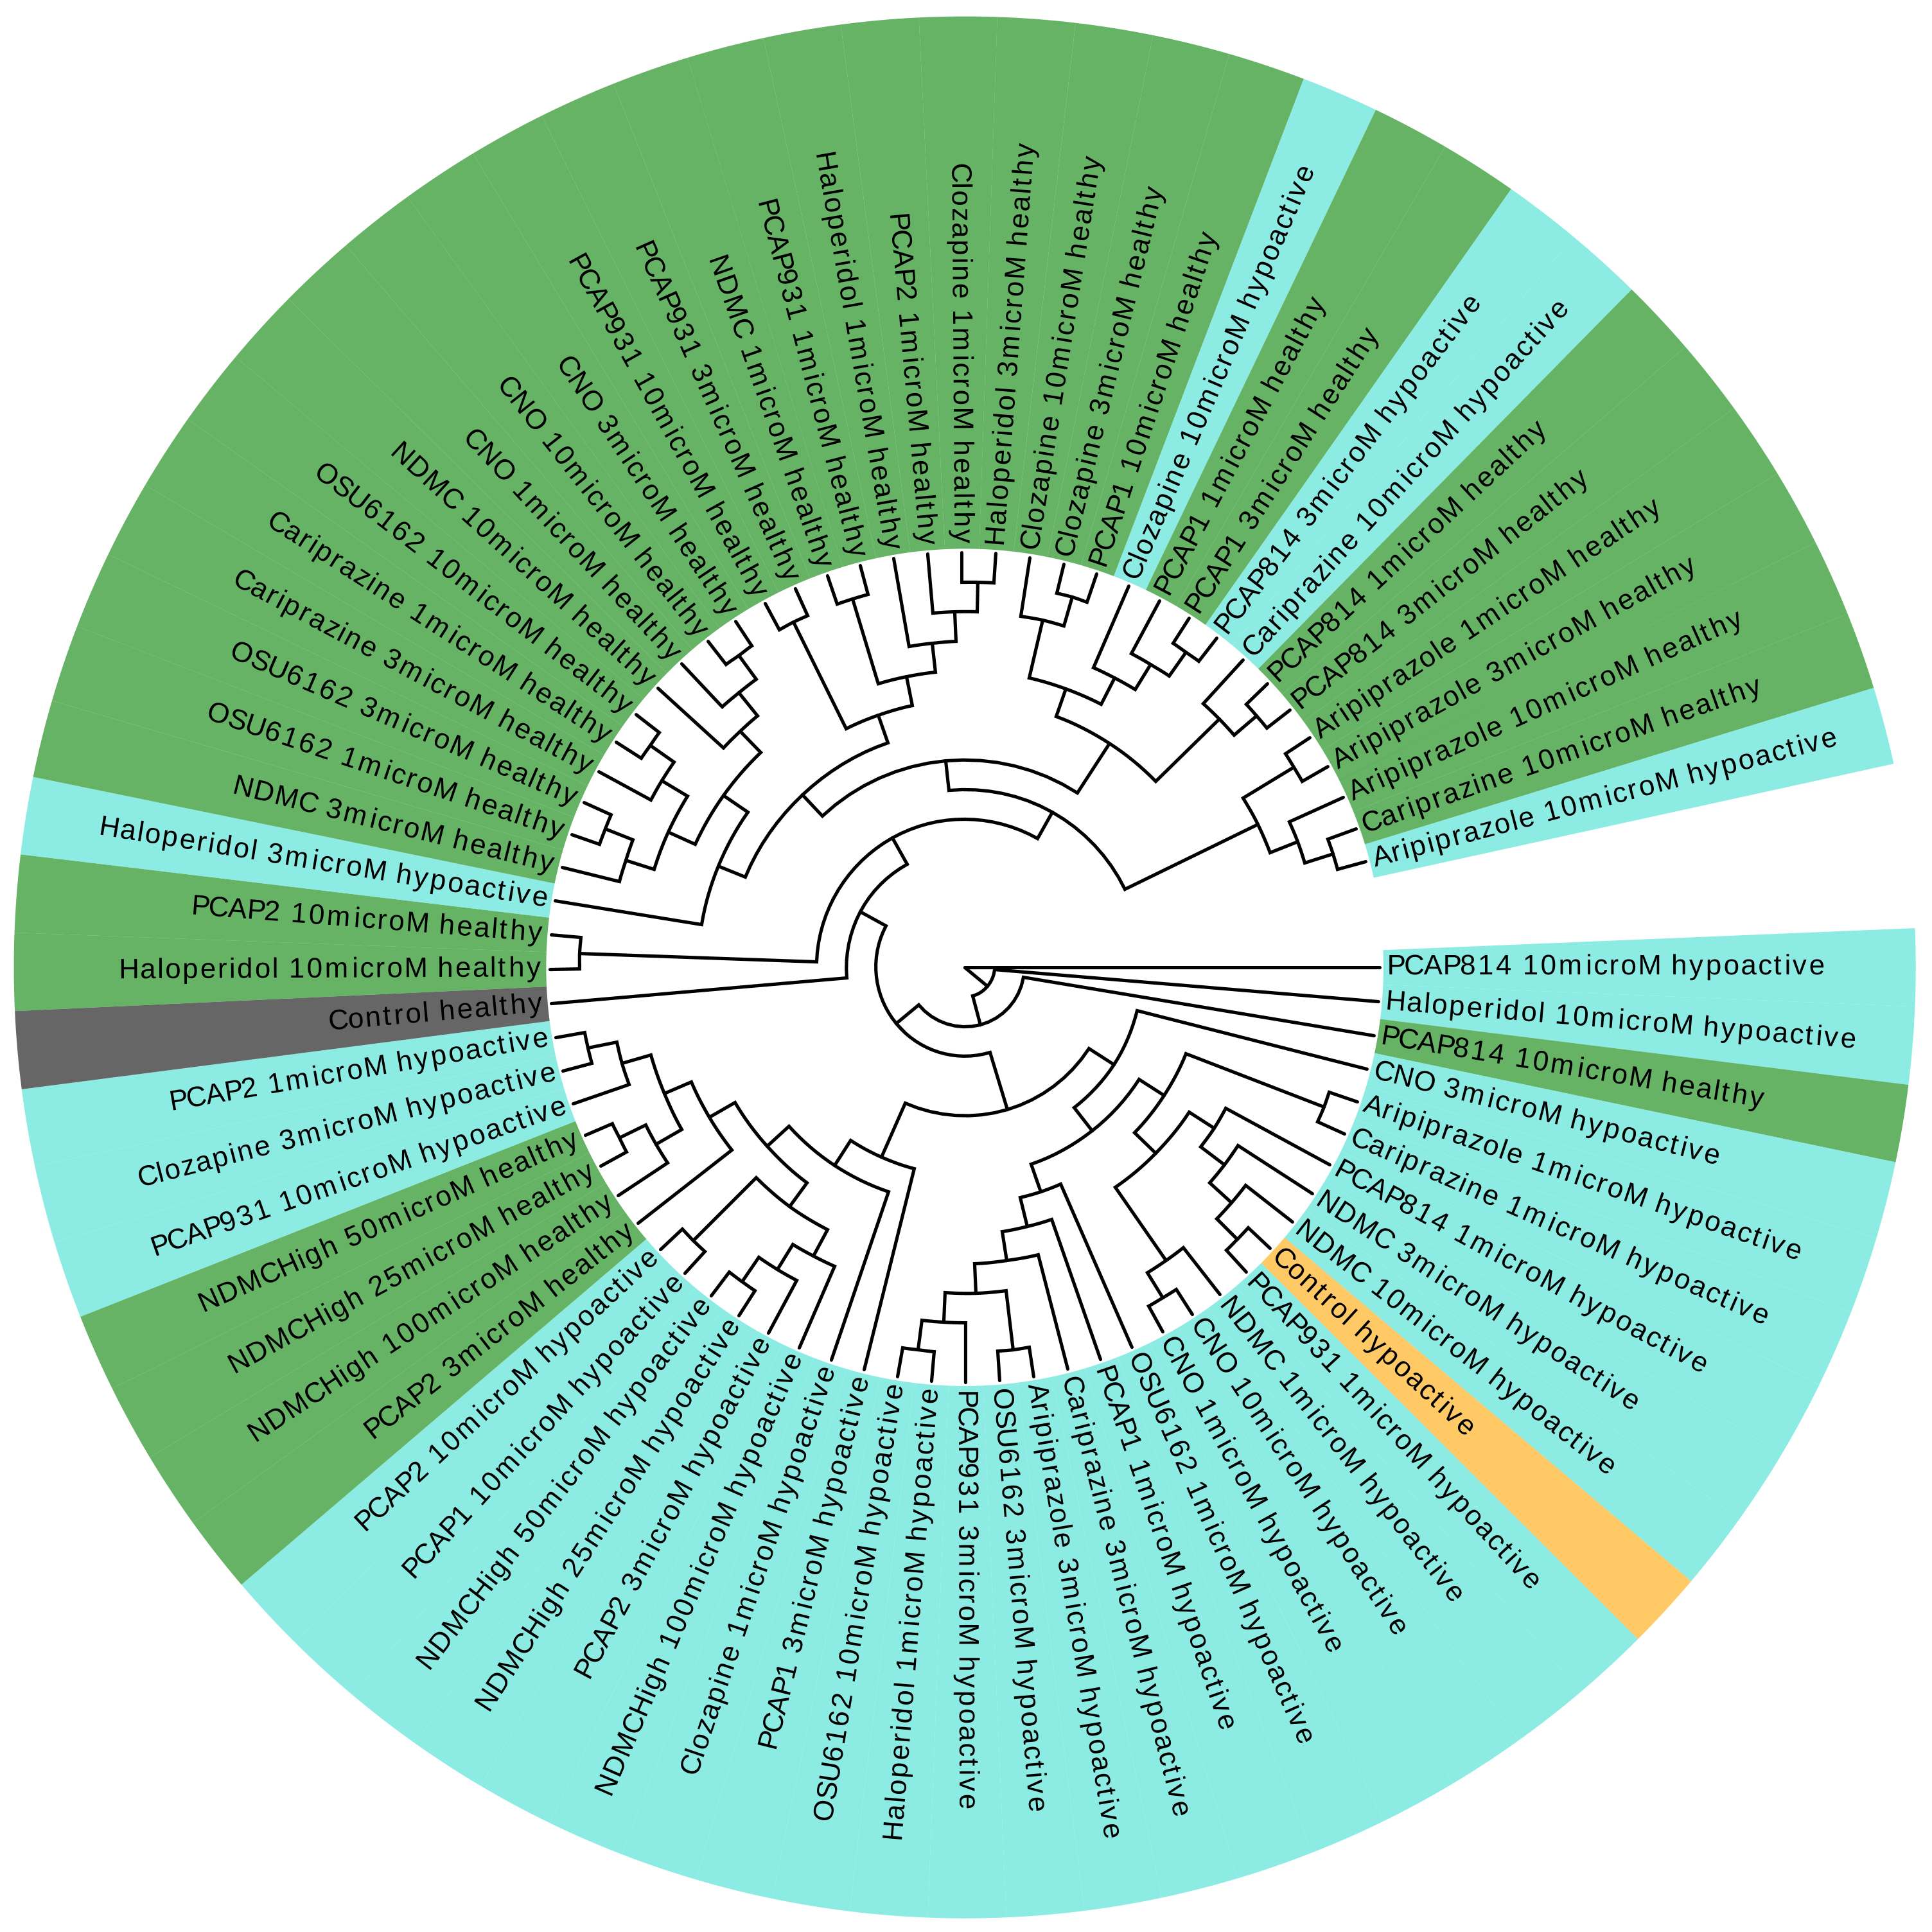
\includegraphics[width=8cm,height=7.5cm]{DarkApoLow_set4_PCA_tree.png}
\caption{Circular cladogram, representing Euclidean distances between the first five principal components of all experimental groups in the healthy and hypoactive condition, using the fourth set of descriptive statistics.}
\end{center}
\end{figure}
\begin{figure}[h!]
\begin{center}
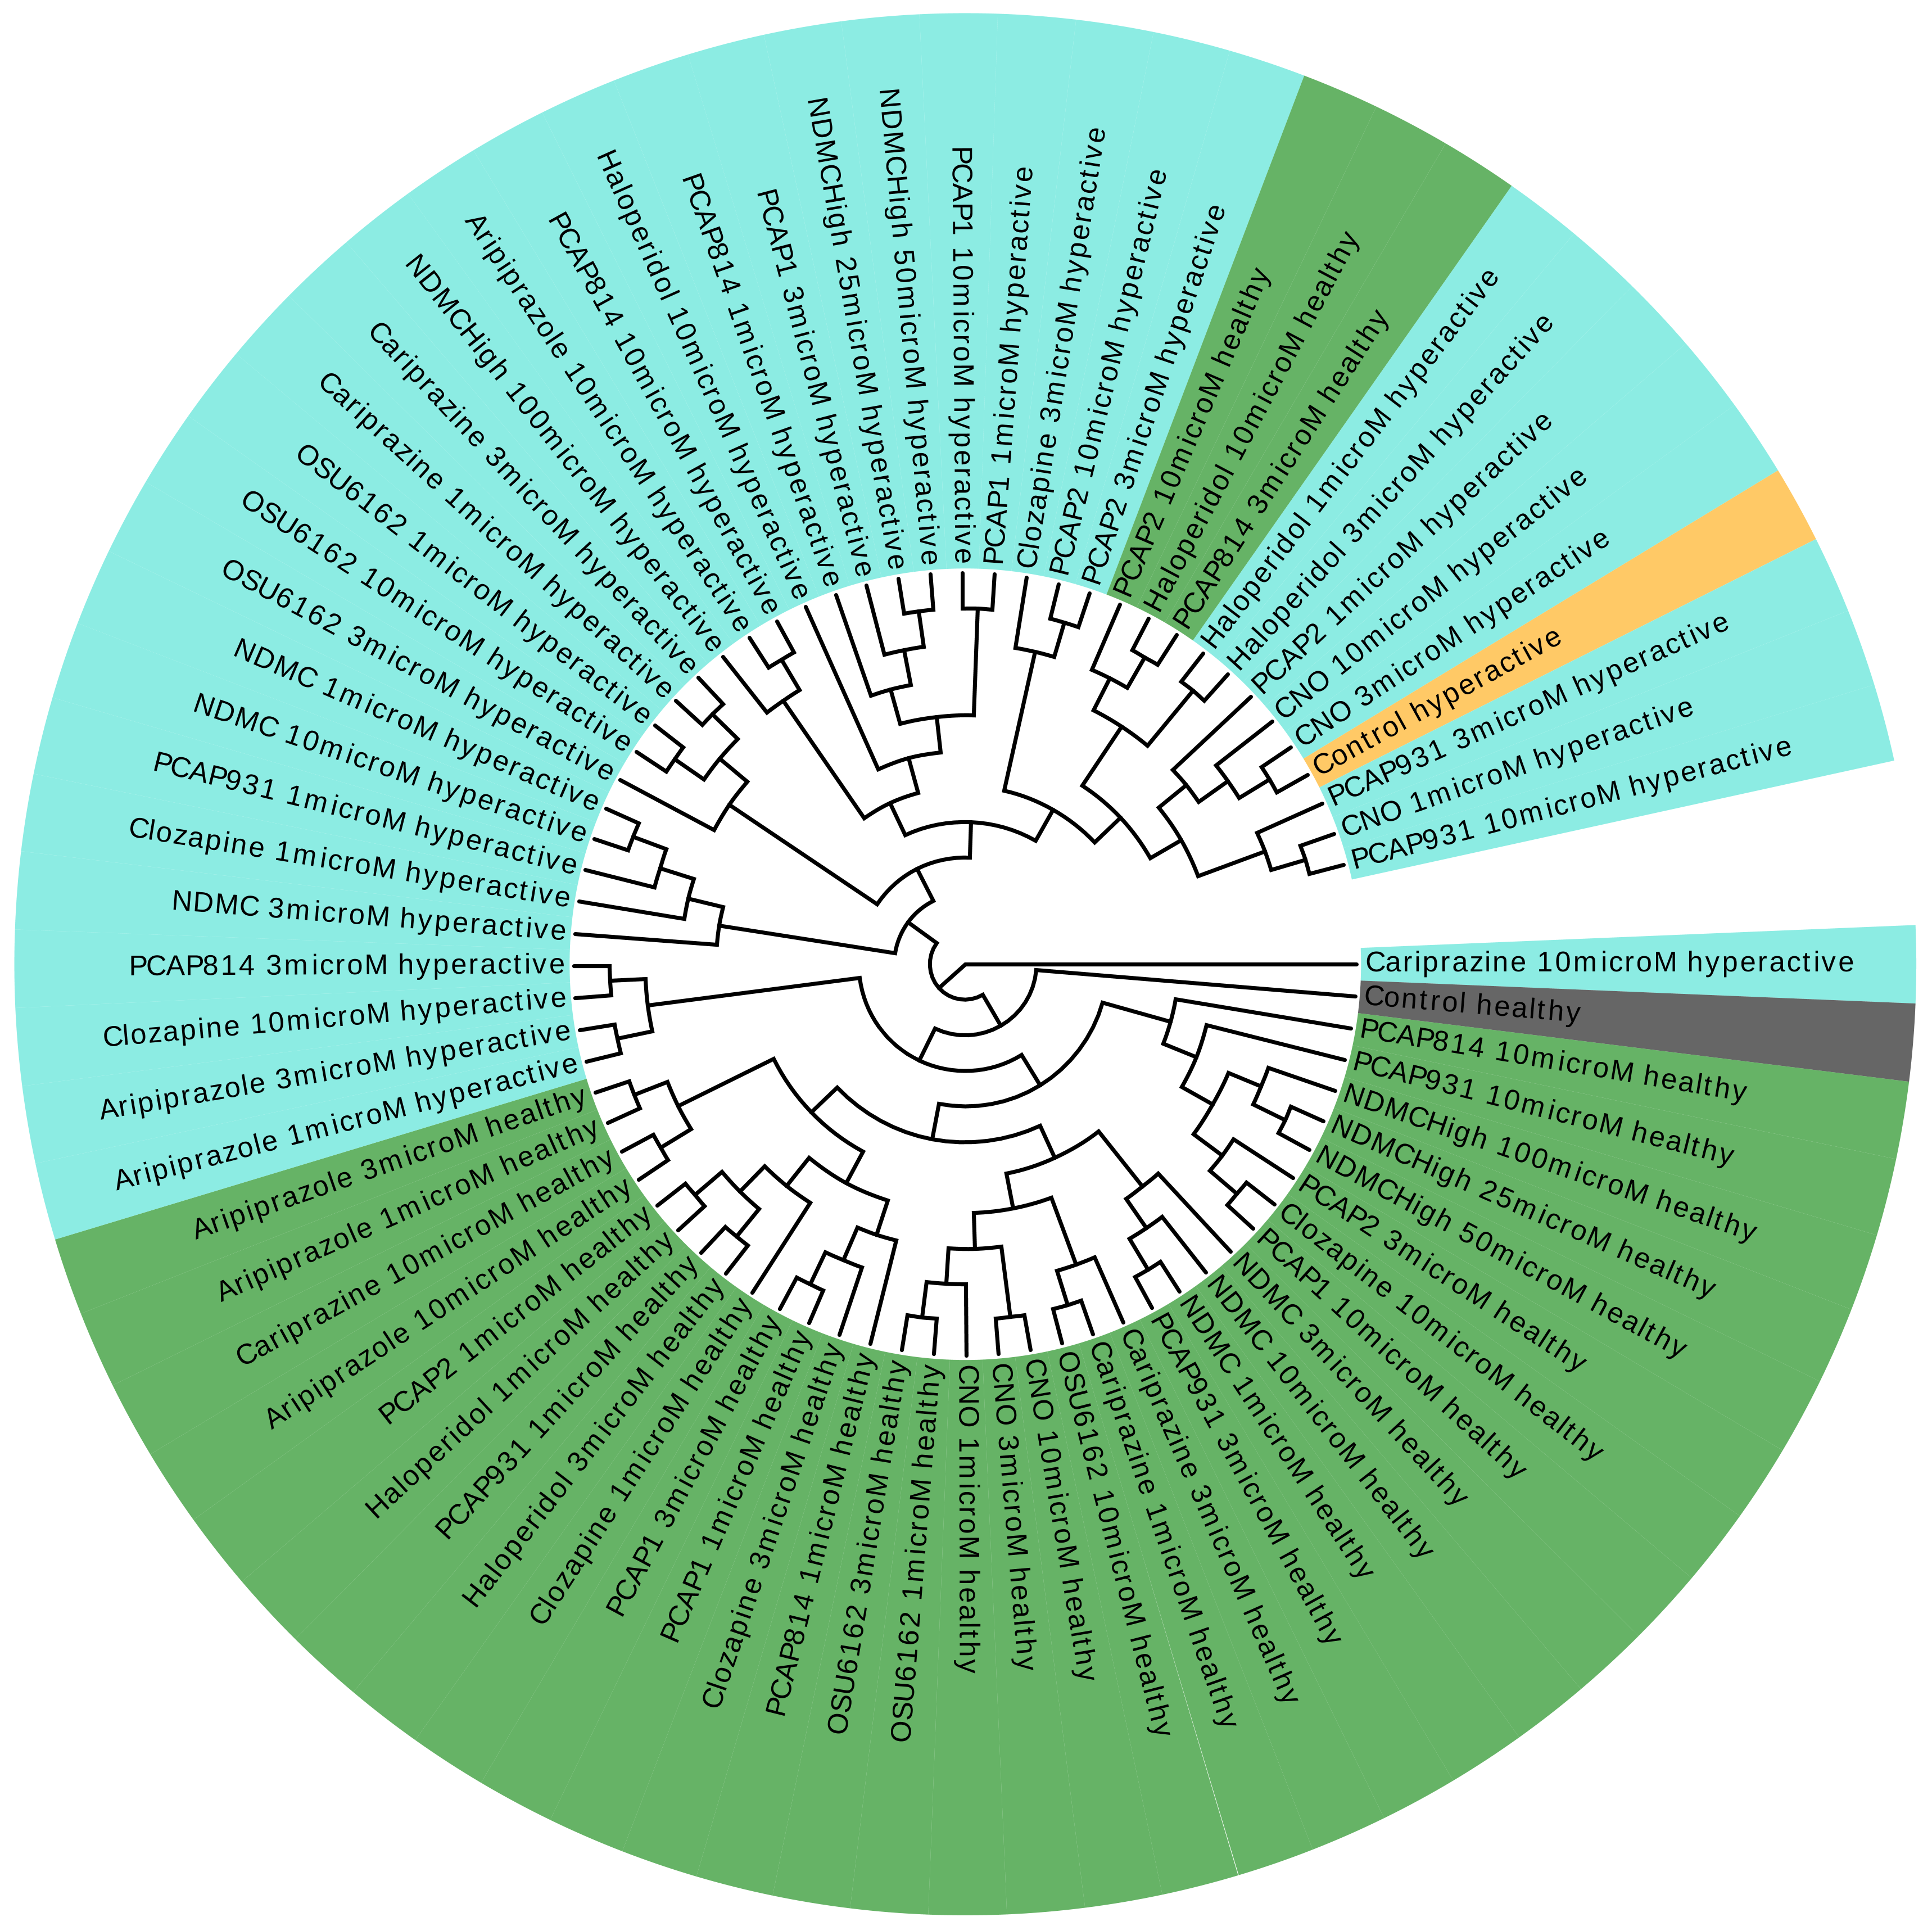
\includegraphics[width=8cm,height=7.5cm]{DarkApoHigh_set4_PCA_tree.png}
\caption{Circular cladogram, representing Euclidean distances between the first five principal components of all experimental groups in the healthy and type I hyperactive condition, using the fourth set of descriptive statistics.}
\end{center}
\end{figure}
\begin{figure}[h!]
\begin{center}
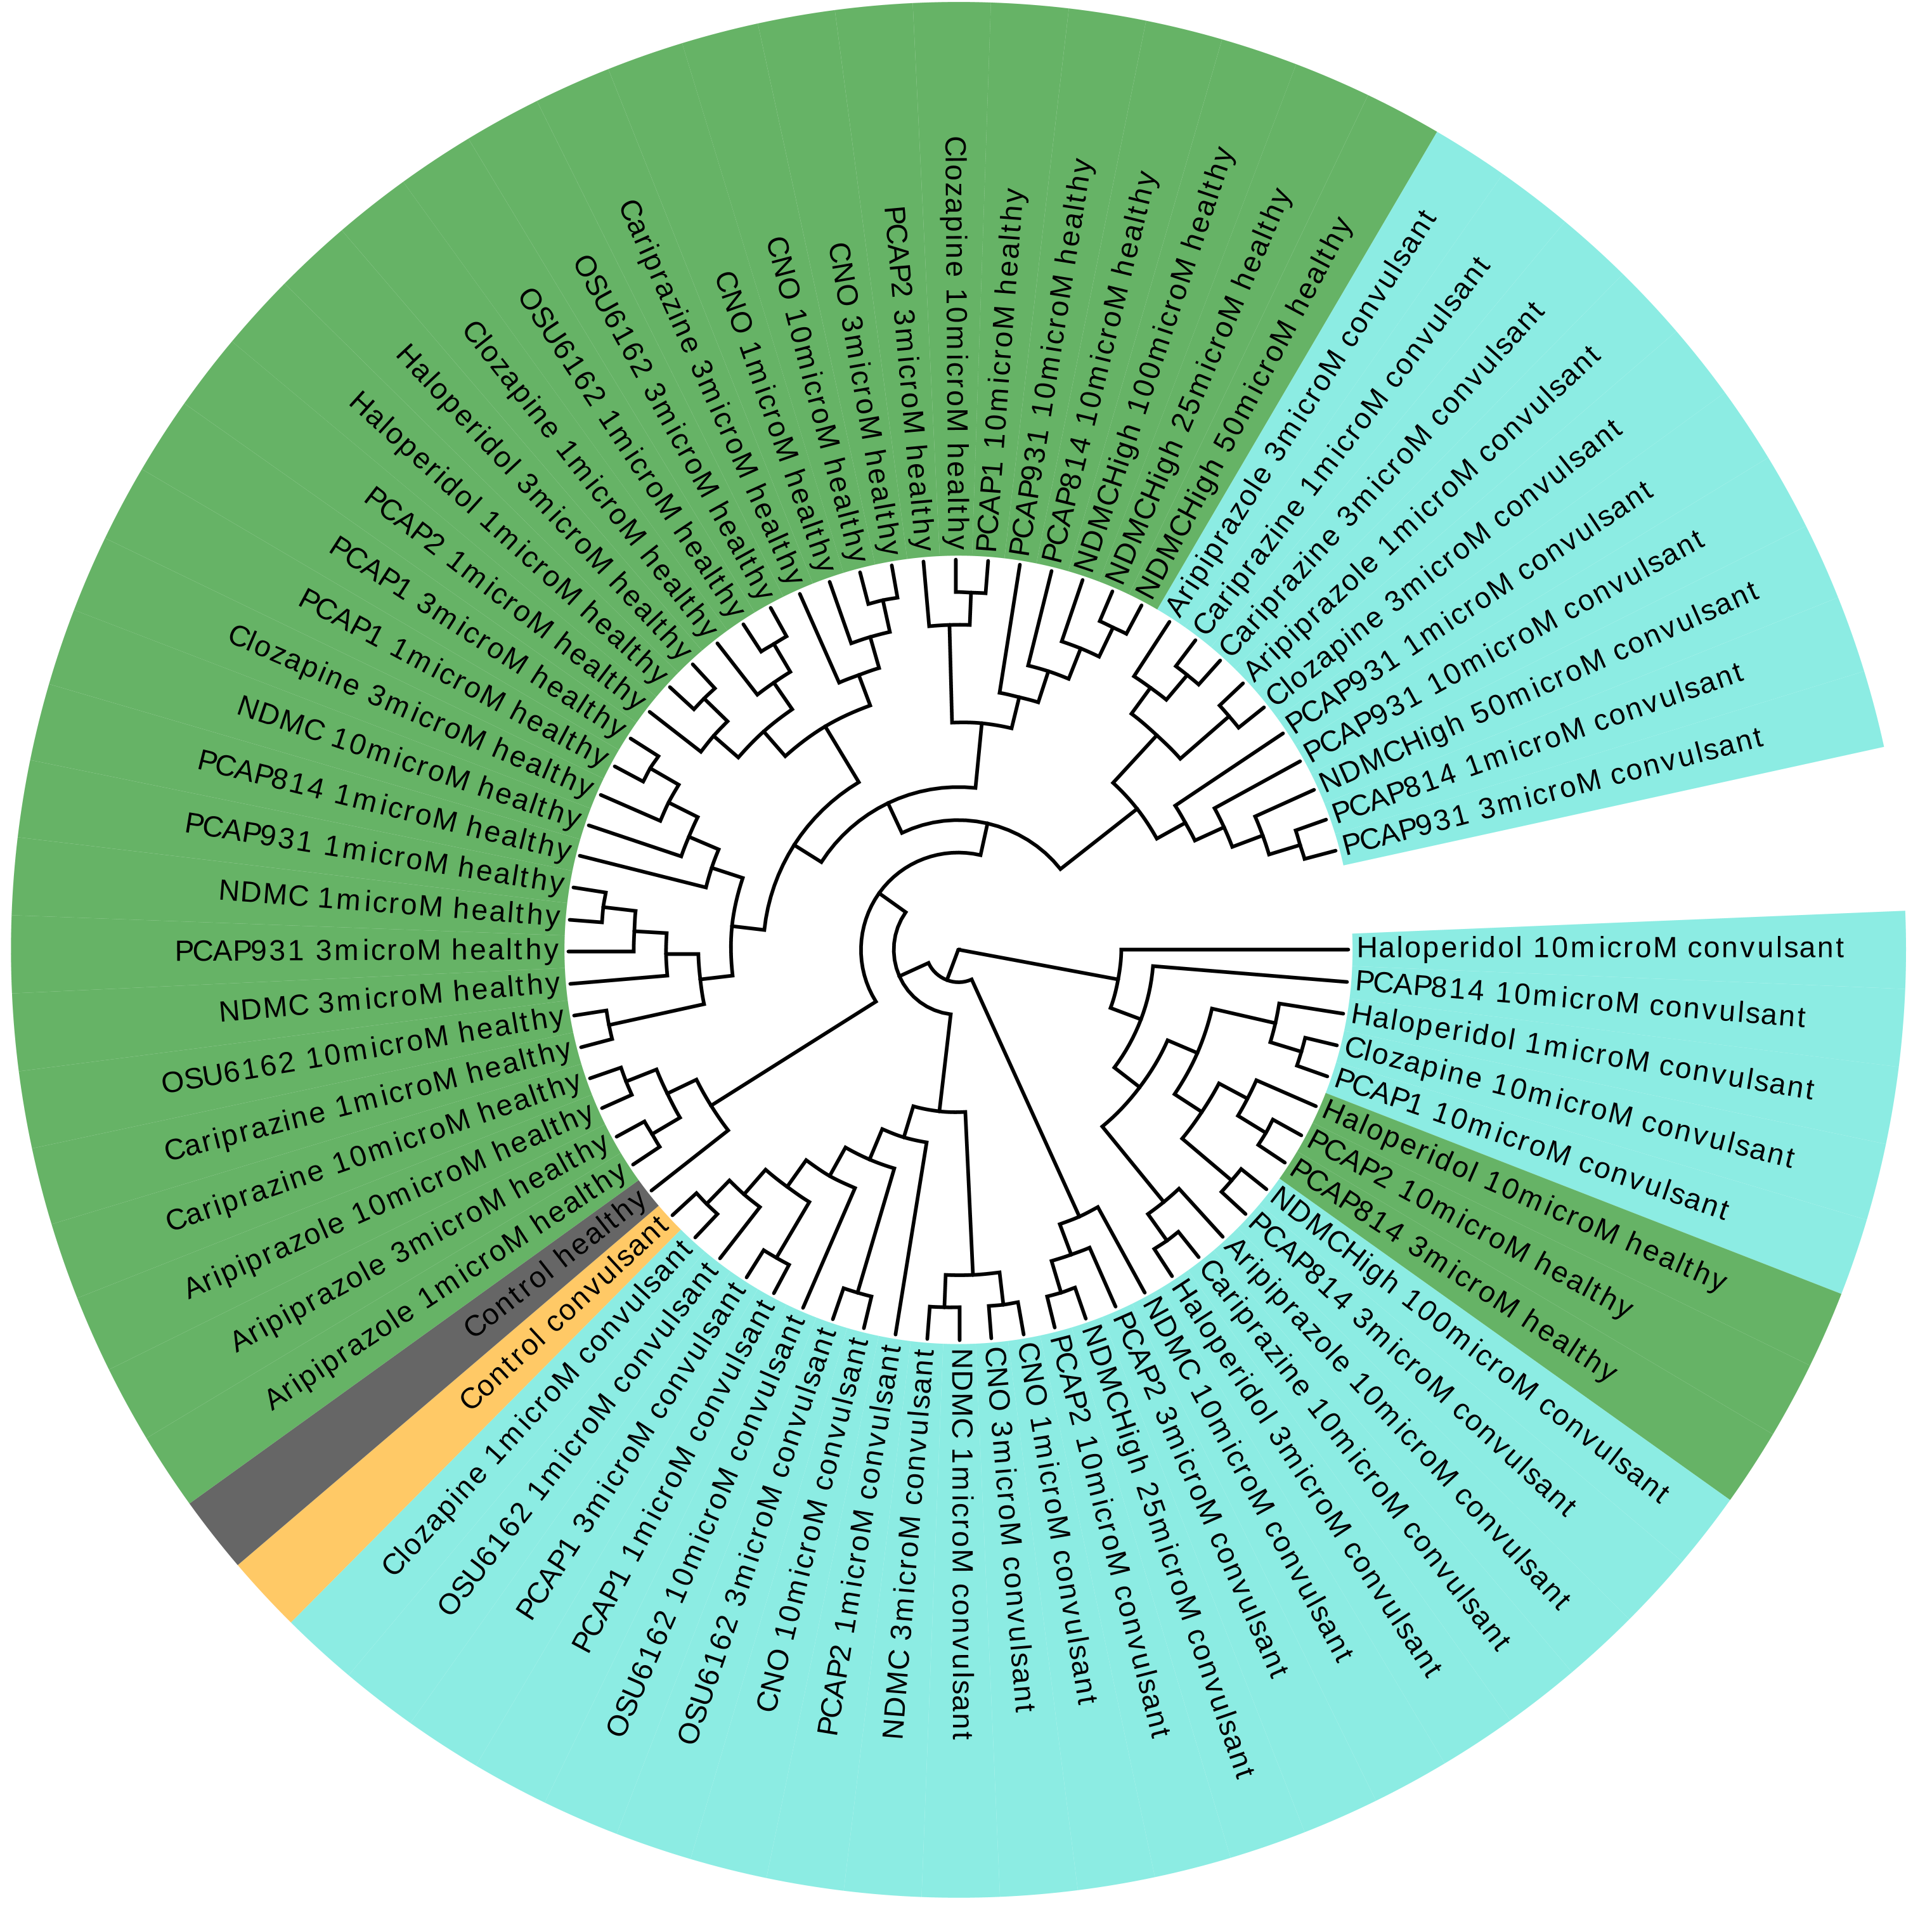
\includegraphics[width=8cm,height=7.5cm]{DarkPTZ_set4_PCA_tree.png}
\caption{Circular cladogram, representing Euclidean distances between the first five principal components of all experimental groups in the healthy and type II hyperactive condition, using the fourth set of descriptive statistics.}
\end{center}
\end{figure}
